\documentclass[twoside]{book}

% Packages required by doxygen
\usepackage{fixltx2e}
\usepackage{calc}
\usepackage{doxygen}
\usepackage[export]{adjustbox} % also loads graphicx
\usepackage{graphicx}
\usepackage[utf8]{inputenc}
\usepackage{makeidx}
\usepackage{multicol}
\usepackage{multirow}
\PassOptionsToPackage{warn}{textcomp}
\usepackage{textcomp}
\usepackage[nointegrals]{wasysym}
\usepackage[table]{xcolor}

% Font selection
\usepackage[T1]{fontenc}
\usepackage[scaled=.90]{helvet}
\usepackage{courier}
\usepackage{amssymb}
\usepackage{sectsty}
\renewcommand{\familydefault}{\sfdefault}
\allsectionsfont{%
  \fontseries{bc}\selectfont%
  \color{darkgray}%
}
\renewcommand{\DoxyLabelFont}{%
  \fontseries{bc}\selectfont%
  \color{darkgray}%
}
\newcommand{\+}{\discretionary{\mbox{\scriptsize$\hookleftarrow$}}{}{}}

% Page & text layout
\usepackage{geometry}
\geometry{%
  a4paper,%
  top=2.5cm,%
  bottom=2.5cm,%
  left=2.5cm,%
  right=2.5cm%
}
\tolerance=750
\hfuzz=15pt
\hbadness=750
\setlength{\emergencystretch}{15pt}
\setlength{\parindent}{0cm}
\setlength{\parskip}{3ex plus 2ex minus 2ex}
\makeatletter
\renewcommand{\paragraph}{%
  \@startsection{paragraph}{4}{0ex}{-1.0ex}{1.0ex}{%
    \normalfont\normalsize\bfseries\SS@parafont%
  }%
}
\renewcommand{\subparagraph}{%
  \@startsection{subparagraph}{5}{0ex}{-1.0ex}{1.0ex}{%
    \normalfont\normalsize\bfseries\SS@subparafont%
  }%
}
\makeatother

% Headers & footers
\usepackage{fancyhdr}
\pagestyle{fancyplain}
\fancyhead[LE]{\fancyplain{}{\bfseries\thepage}}
\fancyhead[CE]{\fancyplain{}{}}
\fancyhead[RE]{\fancyplain{}{\bfseries\leftmark}}
\fancyhead[LO]{\fancyplain{}{\bfseries\rightmark}}
\fancyhead[CO]{\fancyplain{}{}}
\fancyhead[RO]{\fancyplain{}{\bfseries\thepage}}
\fancyfoot[LE]{\fancyplain{}{}}
\fancyfoot[CE]{\fancyplain{}{}}
\fancyfoot[RE]{\fancyplain{}{\bfseries\scriptsize Generated by Doxygen }}
\fancyfoot[LO]{\fancyplain{}{\bfseries\scriptsize Generated by Doxygen }}
\fancyfoot[CO]{\fancyplain{}{}}
\fancyfoot[RO]{\fancyplain{}{}}
\renewcommand{\footrulewidth}{0.4pt}
\renewcommand{\chaptermark}[1]{%
  \markboth{#1}{}%
}
\renewcommand{\sectionmark}[1]{%
  \markright{\thesection\ #1}%
}

% Indices & bibliography
\usepackage{natbib}
\usepackage[titles]{tocloft}
\setcounter{tocdepth}{3}
\setcounter{secnumdepth}{5}
\makeindex

% Custom commands
\newcommand{\clearemptydoublepage}{%
  \newpage{\pagestyle{empty}\cleardoublepage}%
}

\usepackage{caption}
\captionsetup{labelsep=space,justification=centering,font={bf},singlelinecheck=off,skip=4pt,position=top}

%===== C O N T E N T S =====

\begin{document}

% Titlepage & ToC
\pagenumbering{alph}
\begin{titlepage}
\vspace*{7cm}
\begin{center}%
{\Large kakuro }\\
\vspace*{1cm}
{\large Generated by Doxygen 1.8.13}\\
\end{center}
\end{titlepage}
\clearemptydoublepage
\pagenumbering{roman}
\tableofcontents
\clearemptydoublepage
\pagenumbering{arabic}

%--- Begin generated contents ---
\chapter{Hierarchical Index}
\section{Class Hierarchy}
This inheritance list is sorted roughly, but not completely, alphabetically\+:\begin{DoxyCompactList}
\item \contentsline{section}{Capa\+Dominio\+Kakuro}{\pageref{class_dominio_1_1controladores_1_1_capa_dominio_kakuro}}{}
\begin{DoxyCompactList}
\item \contentsline{section}{Driver\+Capa\+Dominio\+Kakuro}{\pageref{class_dominio_1_1controladores_1_1_drivers_1_1_driver_capa_dominio_kakuro}}{}
\end{DoxyCompactList}
\item \contentsline{section}{Ctrl\+Capa\+Dominio}{\pageref{class_dominio_1_1controladores_1_1_ctrl_capa_dominio}}{}
\item \contentsline{section}{Ctrl\+Kakuro}{\pageref{class_persistencia_1_1_ctrl_kakuro}}{}
\item \contentsline{section}{Ctrl\+Partida}{\pageref{class_persistencia_1_1_ctrl_partida}}{}
\item \contentsline{section}{Ctrl\+Persistencia}{\pageref{class_persistencia_1_1_ctrl_persistencia}}{}
\item \contentsline{section}{Ctrl\+Presentacion}{\pageref{class_presentacion_1_1_ctrl_presentacion}}{}
\item \contentsline{section}{Ctrl\+Ranking}{\pageref{class_persistencia_1_1_ctrl_ranking}}{}
\item \contentsline{section}{Ctrl\+Registro}{\pageref{class_persistencia_1_1_ctrl_registro}}{}
\item J\+Dialog\begin{DoxyCompactList}
\item \contentsline{section}{Guardar\+Partida\+Dialog}{\pageref{class_presentacion_1_1_guardar_partida_dialog}}{}
\end{DoxyCompactList}
\item J\+Panel\begin{DoxyCompactList}
\item \contentsline{section}{Vista\+Cargar\+Partida}{\pageref{class_presentacion_1_1_vista_cargar_partida}}{}
\item \contentsline{section}{Vista\+Crear\+Kakuro}{\pageref{class_presentacion_1_1_vista_crear_kakuro}}{}
\item \contentsline{section}{Vista\+Kakuro}{\pageref{class_presentacion_1_1_vista_kakuro}}{}
\item \contentsline{section}{Vista\+Login}{\pageref{class_presentacion_1_1_vista_login}}{}
\item \contentsline{section}{Vista\+Menu\+Principal}{\pageref{class_presentacion_1_1_vista_menu_principal}}{}
\item \contentsline{section}{Vista\+Nueva\+Partida}{\pageref{class_presentacion_1_1_vista_nueva_partida}}{}
\item \contentsline{section}{Vista\+Partida}{\pageref{class_presentacion_1_1_vista_partida}}{}
\item \contentsline{section}{Vista\+Ranking}{\pageref{class_presentacion_1_1_vista_ranking}}{}
\item \contentsline{section}{Vista\+Seleccionar\+Kakuro}{\pageref{class_presentacion_1_1_vista_seleccionar_kakuro}}{}
\item \contentsline{section}{Vista\+Sign\+Up}{\pageref{class_presentacion_1_1_vista_sign_up}}{}
\end{DoxyCompactList}
\item \contentsline{section}{Kakuro\+\_\+\+Game}{\pageref{class_dominio_1_1clases_1_1_kakuro___game}}{}
\item \contentsline{section}{Vista\+Gestion\+Perfil}{\pageref{class_presentacion_1_1_vista_gestion_perfil}}{}
\item \contentsline{section}{Vista\+Principal}{\pageref{class_presentacion_1_1_vista_principal}}{}
\item Serializable\begin{DoxyCompactList}
\item \contentsline{section}{Casilla}{\pageref{class_dominio_1_1clases_1_1_casilla}}{}
\item \contentsline{section}{Kakuro}{\pageref{class_dominio_1_1clases_1_1_kakuro}}{}
\item \contentsline{section}{partida}{\pageref{class_dominio_1_1clases_1_1partida}}{}
\begin{DoxyCompactList}
\item \contentsline{section}{Driver\+Partida}{\pageref{class_dominio_1_1controladores_1_1_drivers_1_1_driver_partida}}{}
\end{DoxyCompactList}
\end{DoxyCompactList}
\end{DoxyCompactList}

\chapter{Data Structure Index}
\section{Data Structures}
Here are the data structures with brief descriptions\+:\begin{DoxyCompactList}
\item\contentsline{section}{\textbf{ Capa\+Dominio\+Kakuro} \\*Clase donde implementamos las funcionalidades principales del programa, siendo estas validar, generar y solucionar un Kakuro }{\pageref{class_dominio_1_1controladores_1_1_capa_dominio_kakuro}}{}
\item\contentsline{section}{\textbf{ Casilla} \\*Clase que representa una \doxyref{Casilla}{p.}{class_dominio_1_1clases_1_1_casilla} de un tablero de un \doxyref{Kakuro}{p.}{class_dominio_1_1clases_1_1_kakuro} }{\pageref{class_dominio_1_1clases_1_1_casilla}}{}
\item\contentsline{section}{\textbf{ Ctrl\+Capa\+Dominio} \\*Clase que se utiliza como intermediaria entre presentacion y persistencia. Transforma los datos que recibe de persistencia y se los pasa a presentacion }{\pageref{class_dominio_1_1controladores_1_1_ctrl_capa_dominio}}{}
\item\contentsline{section}{\textbf{ Ctrl\+Kakuro} \\*Clase que implementa la lectura y escritura de Kakuros en disco }{\pageref{class_persistencia_1_1_ctrl_kakuro}}{}
\item\contentsline{section}{\textbf{ Ctrl\+Partida} \\*Clase que implementa la lectura y escritura de partidas en disco }{\pageref{class_persistencia_1_1_ctrl_partida}}{}
\item\contentsline{section}{\textbf{ Ctrl\+Persistencia} \\*Clase que se encarga de recibir consultas y enviar datos a las demás capas de proyecto. éstas consultas las llevará a la clase indicada y devolverá su resultado }{\pageref{class_persistencia_1_1_ctrl_persistencia}}{}
\item\contentsline{section}{\textbf{ Ctrl\+Presentacion} \\*Clase que inicializa todos los controladores de presentación y contiene las funcionalidades necesarias para llevar a cabo la función explicada anteriormente }{\pageref{class_presentacion_1_1_ctrl_presentacion}}{}
\item\contentsline{section}{\textbf{ Ctrl\+Ranking} \\*Clase que implementa la lectura y escritura del Ranking en disco }{\pageref{class_persistencia_1_1_ctrl_ranking}}{}
\item\contentsline{section}{\textbf{ Ctrl\+Registro} \\*Clase que implementa la lectura y escritura del registro de usuarios en disco }{\pageref{class_persistencia_1_1_ctrl_registro}}{}
\item\contentsline{section}{\textbf{ Driver\+Capa\+Dominio\+Kakuro} }{\pageref{class_dominio_1_1controladores_1_1_drivers_1_1_driver_capa_dominio_kakuro}}{}
\item\contentsline{section}{\textbf{ Driver\+Partida} }{\pageref{class_dominio_1_1controladores_1_1_drivers_1_1_driver_partida}}{}
\item\contentsline{section}{\textbf{ Guardar\+Partida\+Dialog} \\*Clase que implementa el diálogo para poner nombre a una partida guardada }{\pageref{class_presentacion_1_1_guardar_partida_dialog}}{}
\item\contentsline{section}{\textbf{ Kakuro} \\*Clase que representa un kakuro. Contiene su tablero tanto información sobre el mismo }{\pageref{class_dominio_1_1clases_1_1_kakuro}}{}
\item\contentsline{section}{\textbf{ Kakuro\+\_\+\+Game} }{\pageref{class_dominio_1_1clases_1_1_kakuro___game}}{}
\item\contentsline{section}{\textbf{ partida} \\*Clase que representa una partida. Cada partida consiste en el id del usuario que la guarda, un identificador de partida, el tiempo transcurrido y el \doxyref{Kakuro}{p.}{class_dominio_1_1clases_1_1_kakuro} en juego }{\pageref{class_dominio_1_1clases_1_1partida}}{}
\item\contentsline{section}{\textbf{ Vista\+Cargar\+Partida} \\*Clase que extiende J\+Panel que inicializa, gestiona y modifica el panel de la \doxyref{Vista\+Principal}{p.}{class_presentacion_1_1_vista_principal} para Cargar Partidas }{\pageref{class_presentacion_1_1_vista_cargar_partida}}{}
\item\contentsline{section}{\textbf{ Vista\+Crear\+Kakuro} \\*Clase que extiende J\+Panel que inicializa, gestiona y modifica el panel de la \doxyref{Vista\+Principal}{p.}{class_presentacion_1_1_vista_principal} para Crear Kakuros }{\pageref{class_presentacion_1_1_vista_crear_kakuro}}{}
\item\contentsline{section}{\textbf{ Vista\+Gestion\+Perfil} \\*Clase que inicializa, gestiona y modifica la Vista que controla el inicio de sesión y registro en el programa }{\pageref{class_presentacion_1_1_vista_gestion_perfil}}{}
\item\contentsline{section}{\textbf{ Vista\+Kakuro} \\*Clase que extiende J\+Panel que inicializa, gestiona y modifica el panel de la \doxyref{Vista\+Principal}{p.}{class_presentacion_1_1_vista_principal} para jugar un Kakuro }{\pageref{class_presentacion_1_1_vista_kakuro}}{}
\item\contentsline{section}{\textbf{ Vista\+Login} \\*Clase que extiende J\+Panel que inicializa, gestiona y modifica el panel de la \doxyref{Vista\+Gestion\+Perfil}{p.}{class_presentacion_1_1_vista_gestion_perfil} para iniciar sesión }{\pageref{class_presentacion_1_1_vista_login}}{}
\item\contentsline{section}{\textbf{ Vista\+Menu\+Principal} \\*Clase que extiende J\+Panel que inicializa, gestiona y modifica el panel de la \doxyref{Vista\+Principal}{p.}{class_presentacion_1_1_vista_principal} para mostrar el menú principal }{\pageref{class_presentacion_1_1_vista_menu_principal}}{}
\item\contentsline{section}{\textbf{ Vista\+Nueva\+Partida} \\*Clase que extiende J\+Panel que inicializa, gestiona y modifica el panel de la \doxyref{Vista\+Principal}{p.}{class_presentacion_1_1_vista_principal} para jugar una nueva partida }{\pageref{class_presentacion_1_1_vista_nueva_partida}}{}
\item\contentsline{section}{\textbf{ Vista\+Partida} \\*Clase que extiende J\+Panel que inicializa, gestiona y modifica el panel de la \doxyref{Vista\+Principal}{p.}{class_presentacion_1_1_vista_principal} para jugar una partida }{\pageref{class_presentacion_1_1_vista_partida}}{}
\item\contentsline{section}{\textbf{ Vista\+Principal} \\*Clase que inicializa todos los paneles de la vista, además de gestionar el cambio entre paneles y su correcto funcionamiento. también transmite y recibe las solicitudes de datos y sus resultados para los paneles que gestiona }{\pageref{class_presentacion_1_1_vista_principal}}{}
\item\contentsline{section}{\textbf{ Vista\+Ranking} \\*Clase que extiende J\+Panel que inicializa, gestiona y modifica el panel de la \doxyref{Vista\+Principal}{p.}{class_presentacion_1_1_vista_principal} para consultar el ranking }{\pageref{class_presentacion_1_1_vista_ranking}}{}
\item\contentsline{section}{\textbf{ Vista\+Seleccionar\+Kakuro} \\*Clase que extiende J\+Panel que inicializa, gestiona y modifica el panel de la \doxyref{Vista\+Principal}{p.}{class_presentacion_1_1_vista_principal} para Seleccionar un kakuro ya existente mediante su ID }{\pageref{class_presentacion_1_1_vista_seleccionar_kakuro}}{}
\item\contentsline{section}{\textbf{ Vista\+Sign\+Up} }{\pageref{class_presentacion_1_1_vista_sign_up}}{}
\end{DoxyCompactList}

\chapter{File Index}
\section{File List}
Here is a list of all documented files with brief descriptions\+:\begin{DoxyCompactList}
\item\contentsline{section}{src/\+Dominio/clases/\textbf{ Casilla.\+java} \\*Archivo que implementa la clase Casilla }{\pageref{_casilla_8java}}{}
\item\contentsline{section}{src/\+Dominio/clases/\textbf{ Kakuro.\+java} \\*Archivo que implementa la clase Kakuro }{\pageref{_kakuro_8java}}{}
\item\contentsline{section}{src/\+Dominio/clases/\textbf{ Kakuro\+\_\+\+Game.\+java} \\*Archivo principal del programa }{\pageref{_kakuro___game_8java}}{}
\item\contentsline{section}{src/\+Dominio/clases/\textbf{ partida.\+java} \\*Archivo que implementa la clase partida }{\pageref{partida_8java}}{}
\item\contentsline{section}{src/\+Dominio/controladores/\textbf{ Capa\+Dominio\+Kakuro.\+java} \\*Archivo que contiene las funcionalidades principales del programa }{\pageref{_capa_dominio_kakuro_8java}}{}
\item\contentsline{section}{src/\+Dominio/controladores/\textbf{ Ctrl\+Capa\+Dominio.\+java} \\*Controlador que interactúa con la capa de dominio y se encarga de pasar datos con las demás capas }{\pageref{_ctrl_capa_dominio_8java}}{}
\item\contentsline{section}{src/\+Dominio/controladores/\+Drivers/{\bfseries Driver\+Capa\+Dominio\+Kakuro.\+java} }{\pageref{_driver_capa_dominio_kakuro_8java}}{}
\item\contentsline{section}{src/\+Dominio/controladores/\+Drivers/{\bfseries Driver\+Partida.\+java} }{\pageref{_driver_partida_8java}}{}
\item\contentsline{section}{src/\+Persistencia/\textbf{ Ctrl\+Kakuro.\+java} \\*Archivo que implementa la lectura y escritura de Kakuros en disco }{\pageref{_ctrl_kakuro_8java}}{}
\item\contentsline{section}{src/\+Persistencia/\textbf{ Ctrl\+Partida.\+java} \\*Archivo que implementa la lectura y escritura de partidas en disco }{\pageref{_ctrl_partida_8java}}{}
\item\contentsline{section}{src/\+Persistencia/\textbf{ Ctrl\+Persistencia.\+java} \\*Archivo que implementa el controlador de la capa de persistencia }{\pageref{_ctrl_persistencia_8java}}{}
\item\contentsline{section}{src/\+Persistencia/\textbf{ Ctrl\+Ranking.\+java} \\*Archivo que implementa la lectura y escritura del Ranking en disco }{\pageref{_ctrl_ranking_8java}}{}
\item\contentsline{section}{src/\+Persistencia/\textbf{ Ctrl\+Registro.\+java} \\*Archivo que implementa la lectura y escritura del registro de usuarios en disco }{\pageref{_ctrl_registro_8java}}{}
\item\contentsline{section}{src/\+Presentacion/\textbf{ Ctrl\+Presentacion.\+java} \\*Controlador de la capa de presentación }{\pageref{_ctrl_presentacion_8java}}{}
\item\contentsline{section}{src/\+Presentacion/{\bfseries Guardar\+Partida\+Dialog.\+java} }{\pageref{_guardar_partida_dialog_8java}}{}
\item\contentsline{section}{src/\+Presentacion/\textbf{ Kakuro\+Grid.\+java} \\*Panel que contiene el Kakuro en Juego }{\pageref{_kakuro_grid_8java}}{}
\item\contentsline{section}{src/\+Presentacion/\textbf{ Kakuro\+Panel.\+java} \\*Panel correspondiente a una casilla del Kakuro en Juego }{\pageref{_kakuro_panel_8java}}{}
\item\contentsline{section}{src/\+Presentacion/\textbf{ Vista\+Cargar\+Partida.\+java} \\*Panel que gestiona la sección de Vista\+Principal para cargar Partidas }{\pageref{_vista_cargar_partida_8java}}{}
\item\contentsline{section}{src/\+Presentacion/\textbf{ Vista\+Crear\+Kakuro.\+java} \\*Panel que gestiona la sección de Vista\+Principal para crear un nuevo Kakuro }{\pageref{_vista_crear_kakuro_8java}}{}
\item\contentsline{section}{src/\+Presentacion/\textbf{ Vista\+Gestion\+Perfil.\+java} \\*Panel que gestiona la Vista de inicio de sesión y registro en el programa }{\pageref{_vista_gestion_perfil_8java}}{}
\item\contentsline{section}{src/\+Presentacion/\textbf{ Vista\+Kakuro.\+java} \\*Panel que gestiona la sección de Vista\+Principal para Jugar un Kakuro }{\pageref{_vista_kakuro_8java}}{}
\item\contentsline{section}{src/\+Presentacion/\textbf{ Vista\+Login.\+java} \\*Panel que gestiona la sección de Vista\+Gestion\+Perfil para iniciar sesión }{\pageref{_vista_login_8java}}{}
\item\contentsline{section}{src/\+Presentacion/\textbf{ Vista\+Menu\+Principal.\+java} \\*Panel que gestiona la sección de Vista\+Principal para mostrar el menú principal }{\pageref{_vista_menu_principal_8java}}{}
\item\contentsline{section}{src/\+Presentacion/\textbf{ Vista\+Nueva\+Partida.\+java} \\*Panel que gestiona la sección de Vista\+Principal para jugar una nueva partida }{\pageref{_vista_nueva_partida_8java}}{}
\item\contentsline{section}{src/\+Presentacion/{\bfseries Vista\+Partida.\+java} }{\pageref{_vista_partida_8java}}{}
\item\contentsline{section}{src/\+Presentacion/\textbf{ Vista\+Principal.\+java} \\*Vista Principal del programa }{\pageref{_vista_principal_8java}}{}
\item\contentsline{section}{src/\+Presentacion/\textbf{ Vista\+Ranking.\+java} \\*Panel que gestiona la sección de Vista\+Principal que muestra el ranking }{\pageref{_vista_ranking_8java}}{}
\item\contentsline{section}{src/\+Presentacion/\textbf{ Vista\+Seleccionar\+Kakuro.\+java} \\*Panel que gestiona la sección de Vista\+Principal para Seleccionar un kakuro ya existente mediante su ID }{\pageref{_vista_seleccionar_kakuro_8java}}{}
\item\contentsline{section}{src/\+Presentacion/\textbf{ Vista\+Sign\+Up.\+java} \\*Panel que gestiona la sección de Vista\+Gestion\+Perfil para registrarse }{\pageref{_vista_sign_up_8java}}{}
\end{DoxyCompactList}

\chapter{Data Structure Documentation}
\section{Capa\+Dominio\+Kakuro Class Reference}
\label{class_dominio_1_1controladores_1_1_capa_dominio_kakuro}\index{Capa\+Dominio\+Kakuro@{Capa\+Dominio\+Kakuro}}


clase donde implementamos las funcionalidades principales del programa, siendo estas validar, generar y solucionar un Kakuro.  




Inheritance diagram for Capa\+Dominio\+Kakuro\+:\nopagebreak
\begin{figure}[H]
\begin{center}
\leavevmode
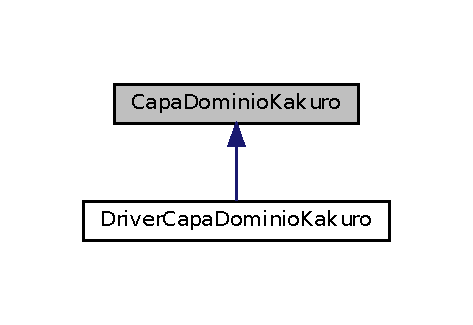
\includegraphics[width=227pt]{class_dominio_1_1controladores_1_1_capa_dominio_kakuro__inherit__graph}
\end{center}
\end{figure}


Collaboration diagram for Capa\+Dominio\+Kakuro\+:
\nopagebreak
\begin{figure}[H]
\begin{center}
\leavevmode
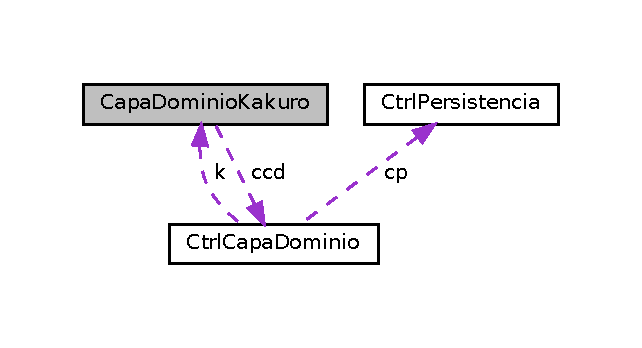
\includegraphics[width=308pt]{class_dominio_1_1controladores_1_1_capa_dominio_kakuro__coll__graph}
\end{center}
\end{figure}
\subsection*{Public Member Functions}
\begin{DoxyCompactItemize}
\item 
\textbf{ Capa\+Dominio\+Kakuro} ()
\begin{DoxyCompactList}\small\item\em Constructora de \doxyref{Capa\+Dominio\+Kakuro}{p.}{class_dominio_1_1controladores_1_1_capa_dominio_kakuro}. \end{DoxyCompactList}\item 
\mbox{\label{class_dominio_1_1controladores_1_1_capa_dominio_kakuro_a4a4657726813077ac245e9f5be0940c4}} 
{\bfseries Capa\+Dominio\+Kakuro} (\textbf{ Ctrl\+Capa\+Dominio} c)
\end{DoxyCompactItemize}
\subsection*{Static Public Member Functions}
\begin{DoxyCompactItemize}
\item 
static int \textbf{ comprobar\+\_\+movimiento} (int i, int j, int v, \textbf{ Kakuro} k)
\begin{DoxyCompactList}\small\item\em funcionalidad utilizada a la hora de jugar que comprueba la validez de un movimiento. \end{DoxyCompactList}\item 
static boolean \textbf{ check\+Run} (int suma, int valor\+\_\+actual, boolean llena)
\begin{DoxyCompactList}\small\item\em Comprueba la validez de una fila o columna con la sumatoria suma si se le añade el valor valor\+\_\+actual. \end{DoxyCompactList}\item 
static void \textbf{ filtrar\+Sumas} (int max, int length, Set$<$ Integer $>$ possible)
\begin{DoxyCompactList}\small\item\em filtra el conjunto de valores posibles de la celda para una fila o columna con sumatorias que solo admiten combinaciones determinadas de valores \end{DoxyCompactList}\item 
static int \textbf{ take\+Fila} (\textbf{ Casilla}[$\,$][$\,$] state, int valor\+\_\+actual, int celdaf, int celdac, Set$<$ Integer $>$ possible)
\begin{DoxyCompactList}\small\item\em comprueba las restricciones de fila de la casilla consultada en el solve. Ademas comprueba si la fila esta llena y filtra los valores posibles para esa fila. \end{DoxyCompactList}\item 
static int \textbf{ take\+Columna} (\textbf{ Casilla}[$\,$][$\,$] state, int valor\+\_\+actual, int celdaf, int celdac, Set$<$ Integer $>$ possible)
\begin{DoxyCompactList}\small\item\em comprueba las restricciones de columna de la casilla consultada en el solve. Ademas comprueba si la columna esta llena y filtra los valores posibles para esa columna. \end{DoxyCompactList}\item 
static void \textbf{ calc\+Posiciones} (\textbf{ Kakuro} k, int startF, int startC, int[$\,$] fila, int[$\,$] columna)
\begin{DoxyCompactList}\small\item\em Calcula y llena los vectores de enteros con los indices de todas las casillas blancas del kakuro k. \end{DoxyCompactList}\item 
static boolean \textbf{ solve} (\textbf{ Kakuro} k, int opcion)
\begin{DoxyCompactList}\small\item\em opcion = 0\+: comprueba que k tiene solucion y, de ser asi, la guarda en result opcion = 1\+: busca todas las posibles soluciones del Kakuro para comprobar si éste tiene 1 solución o más. \end{DoxyCompactList}\item 
static boolean \textbf{ comprobar\+Solucion} (\textbf{ Kakuro} kakuro1)
\begin{DoxyCompactList}\small\item\em comprueba que la solucion alcanzada despues de jugar un kakuro es valida \end{DoxyCompactList}\item 
static \textbf{ Casilla} [$\,$][$\,$] \textbf{ generar\+Kakuro} (int n, int m, double dificultad)
\begin{DoxyCompactList}\small\item\em Genera una matriz de casillas nueva que equivale a la de un kakuro valido. \end{DoxyCompactList}\item 
static boolean \textbf{ generarK} (int n, int m, int negras, \textbf{ Casilla} [$\,$][$\,$]k)
\begin{DoxyCompactList}\small\item\em funcionalidad de generar\+Kakuro encargada de generar la matriz de casillas \end{DoxyCompactList}\item 
static void \textbf{ generar\+Sumas} (\textbf{ Casilla}[$\,$][$\,$] k)
\begin{DoxyCompactList}\small\item\em funcionalidad de generarK encargada de generar las sumatorias de las filas y columnas \end{DoxyCompactList}\item 
static boolean \textbf{ generar\+Casillas\+Blancas} (\textbf{ Casilla}[$\,$][$\,$] k)
\begin{DoxyCompactList}\small\item\em funcionalidad de generarK encargada de generar las casillas blancas y colocarlas \end{DoxyCompactList}\item 
static boolean \textbf{ valor\+Repetido} (\textbf{ Casilla} [$\,$][$\,$]k, int x, int y, int value)
\begin{DoxyCompactList}\small\item\em Verifica que value en la coordenada (x,y) no esta repetido para la matriz de casillas. \end{DoxyCompactList}\item 
static void \textbf{ generar\+Casillas\+Negras} (\textbf{ Casilla} [$\,$][$\,$]k, int n\+Casillas)
\begin{DoxyCompactList}\small\item\em funcionalidad de generarK encargada de generar las casillas negras y colocarlas \end{DoxyCompactList}\item 
static void \textbf{ print\+Cell\+Matrix} (\textbf{ Casilla} [$\,$][$\,$]k)
\begin{DoxyCompactList}\small\item\em Muestra la matriz de casillas k por pantalla. \end{DoxyCompactList}\item 
static void \textbf{ generar\+Resolver} (int dificultad)
\begin{DoxyCompactList}\small\item\em segun una dificultad, generamos un kakuro y posteriormente llamamos a la funcion solve para que lo resuelva \end{DoxyCompactList}\item 
static int \textbf{ generar} (int dificultad)
\begin{DoxyCompactList}\small\item\em segun una dificultad, generamos un kakuro \end{DoxyCompactList}\item 
static int \textbf{ generar} (int dimensiones, int num\+Casillas\+Negras)
\begin{DoxyCompactList}\small\item\em segun unas dimensiones y el numero de casillas negras generamos un kakuro \end{DoxyCompactList}\item 
static boolean \textbf{ validar\+\_\+kakuro} (\textbf{ Kakuro} k)
\begin{DoxyCompactList}\small\item\em Dado un kakuro k, comprobamos que este sea valido. \end{DoxyCompactList}\item 
static \textbf{ Casilla} [$\,$][$\,$] \textbf{ get\+Result} ()
\begin{DoxyCompactList}\small\item\em devuelve el resultado de la solucion \end{DoxyCompactList}\end{DoxyCompactItemize}
\subsection*{Static Public Attributes}
\begin{DoxyCompactItemize}
\item 
\mbox{\label{class_dominio_1_1controladores_1_1_capa_dominio_kakuro_ad9ea4c4f9de31b584323e8b5bf976782}} 
static \textbf{ Ctrl\+Capa\+Dominio} {\bfseries ccd}
\end{DoxyCompactItemize}


\subsection{Detailed Description}
clase donde implementamos las funcionalidades principales del programa, siendo estas validar, generar y solucionar un Kakuro. 

Definition at line 30 of file Capa\+Dominio\+Kakuro.\+java.



\subsection{Constructor \& Destructor Documentation}
\mbox{\label{class_dominio_1_1controladores_1_1_capa_dominio_kakuro_a5f6806ade86e68be838f48b8db9ac68e}} 
\index{Dominio\+::controladores\+::\+Capa\+Dominio\+Kakuro@{Dominio\+::controladores\+::\+Capa\+Dominio\+Kakuro}!Capa\+Dominio\+Kakuro@{Capa\+Dominio\+Kakuro}}
\index{Capa\+Dominio\+Kakuro@{Capa\+Dominio\+Kakuro}!Dominio\+::controladores\+::\+Capa\+Dominio\+Kakuro@{Dominio\+::controladores\+::\+Capa\+Dominio\+Kakuro}}
\subsubsection{Capa\+Dominio\+Kakuro()}
{\footnotesize\ttfamily \textbf{ Capa\+Dominio\+Kakuro} (\begin{DoxyParamCaption}{ }\end{DoxyParamCaption})\hspace{0.3cm}{\ttfamily [inline]}}



Constructora de \doxyref{Capa\+Dominio\+Kakuro}{p.}{class_dominio_1_1controladores_1_1_capa_dominio_kakuro}. 


\begin{DoxyParams}{Parameters}
{\em c} & = Controlador de capa de dominio con el que interactua la clase. \\
\hline
\end{DoxyParams}
\begin{DoxyPostcond}{Postcondition}
Existe una instancia nueva de \doxyref{Capa\+Dominio\+Kakuro}{p.}{class_dominio_1_1controladores_1_1_capa_dominio_kakuro} con el controlador de capa de dominio correspondiente. 
\end{DoxyPostcond}


Definition at line 44 of file Capa\+Dominio\+Kakuro.\+java.



\subsection{Member Function Documentation}
\mbox{\label{class_dominio_1_1controladores_1_1_capa_dominio_kakuro_ac6661a567f7a67bfa3321fb59c65b640}} 
\index{Dominio\+::controladores\+::\+Capa\+Dominio\+Kakuro@{Dominio\+::controladores\+::\+Capa\+Dominio\+Kakuro}!calc\+Posiciones@{calc\+Posiciones}}
\index{calc\+Posiciones@{calc\+Posiciones}!Dominio\+::controladores\+::\+Capa\+Dominio\+Kakuro@{Dominio\+::controladores\+::\+Capa\+Dominio\+Kakuro}}
\subsubsection{calc\+Posiciones()}
{\footnotesize\ttfamily static void calc\+Posiciones (\begin{DoxyParamCaption}\item[{\textbf{ Kakuro}}]{k,  }\item[{int}]{startF,  }\item[{int}]{startC,  }\item[{int [$\,$]}]{fila,  }\item[{int [$\,$]}]{columna }\end{DoxyParamCaption})\hspace{0.3cm}{\ttfamily [inline]}, {\ttfamily [static]}}



Calcula y llena los vectores de enteros con los indices de todas las casillas blancas del kakuro k. 


\begin{DoxyParams}{Parameters}
{\em k} & = kakuro a solucionar \\
\hline
{\em startF} & = fila en la que empieza \\
\hline
{\em startC} & = columna en la que empieza \\
\hline
{\em fila} & = indices de las casillas blancas (fila) \\
\hline
{\em columna} & = indices de las casillas blancas (columna) \\
\hline
\end{DoxyParams}
\begin{DoxyPostcond}{Postcondition}
fila y columna contienen los indices de todas las casillas blancas del kakuro k 
\end{DoxyPostcond}


Definition at line 341 of file Capa\+Dominio\+Kakuro.\+java.

\mbox{\label{class_dominio_1_1controladores_1_1_capa_dominio_kakuro_a2154dd8ec0aa8c9d39bce1616c1b9ae5}} 
\index{Dominio\+::controladores\+::\+Capa\+Dominio\+Kakuro@{Dominio\+::controladores\+::\+Capa\+Dominio\+Kakuro}!check\+Run@{check\+Run}}
\index{check\+Run@{check\+Run}!Dominio\+::controladores\+::\+Capa\+Dominio\+Kakuro@{Dominio\+::controladores\+::\+Capa\+Dominio\+Kakuro}}
\subsubsection{check\+Run()}
{\footnotesize\ttfamily static boolean check\+Run (\begin{DoxyParamCaption}\item[{int}]{suma,  }\item[{int}]{valor\+\_\+actual,  }\item[{boolean}]{llena }\end{DoxyParamCaption})\hspace{0.3cm}{\ttfamily [inline]}, {\ttfamily [static]}}



Comprueba la validez de una fila o columna con la sumatoria suma si se le añade el valor valor\+\_\+actual. 


\begin{DoxyParams}{Parameters}
{\em suma} & = sumatoria de los valores actuales de una fila o columna \\
\hline
{\em valor\+\_\+actual} & = valor a comprobar \\
\hline
{\em llena} & = indica si añadir valor\+\_\+actual llenaría la fila o columna con la sumatoria suma. \\
\hline
\end{DoxyParams}
\begin{DoxyPostcond}{Postcondition}
devuelve cierto o falso dependiendo de la validez de valor\+\_\+actual respecto a la sumatoria suma y el parámetro llena. 
\end{DoxyPostcond}


Definition at line 141 of file Capa\+Dominio\+Kakuro.\+java.

\mbox{\label{class_dominio_1_1controladores_1_1_capa_dominio_kakuro_a01bf443d8d6a2bd070772109fe25ffcf}} 
\index{Dominio\+::controladores\+::\+Capa\+Dominio\+Kakuro@{Dominio\+::controladores\+::\+Capa\+Dominio\+Kakuro}!comprobar\+\_\+movimiento@{comprobar\+\_\+movimiento}}
\index{comprobar\+\_\+movimiento@{comprobar\+\_\+movimiento}!Dominio\+::controladores\+::\+Capa\+Dominio\+Kakuro@{Dominio\+::controladores\+::\+Capa\+Dominio\+Kakuro}}
\subsubsection{comprobar\+\_\+movimiento()}
{\footnotesize\ttfamily static int comprobar\+\_\+movimiento (\begin{DoxyParamCaption}\item[{int}]{i,  }\item[{int}]{j,  }\item[{int}]{v,  }\item[{\textbf{ Kakuro}}]{k }\end{DoxyParamCaption})\hspace{0.3cm}{\ttfamily [inline]}, {\ttfamily [static]}}



funcionalidad utilizada a la hora de jugar que comprueba la validez de un movimiento. 


\begin{DoxyParams}{Parameters}
{\em i} & = fila a comprobar \\
\hline
{\em j} & = columna a comprobar \\
\hline
{\em v} & = valor a comprobar \\
\hline
{\em k} & = kakuro sobre el que realizar las comprobaciones \\
\hline
\end{DoxyParams}
\begin{DoxyPostcond}{Postcondition}
en caso de que el movimiento sea válido, devuelve 4 en caso de que el kakuro esté acabado y 5 en caso de que todavía queden casillas por rellenar. En caso de que el movimiento no sea válido, se devuelve un valor entero diferente dependiendo de la causa del error. 
\end{DoxyPostcond}


Definition at line 64 of file Capa\+Dominio\+Kakuro.\+java.

\mbox{\label{class_dominio_1_1controladores_1_1_capa_dominio_kakuro_a30b5ae4d45535e3b97546c12da259d1d}} 
\index{Dominio\+::controladores\+::\+Capa\+Dominio\+Kakuro@{Dominio\+::controladores\+::\+Capa\+Dominio\+Kakuro}!comprobar\+Solucion@{comprobar\+Solucion}}
\index{comprobar\+Solucion@{comprobar\+Solucion}!Dominio\+::controladores\+::\+Capa\+Dominio\+Kakuro@{Dominio\+::controladores\+::\+Capa\+Dominio\+Kakuro}}
\subsubsection{comprobar\+Solucion()}
{\footnotesize\ttfamily static boolean comprobar\+Solucion (\begin{DoxyParamCaption}\item[{\textbf{ Kakuro}}]{kakuro1 }\end{DoxyParamCaption})\hspace{0.3cm}{\ttfamily [inline]}, {\ttfamily [static]}}



comprueba que la solucion alcanzada despues de jugar un kakuro es valida 


\begin{DoxyParams}{Parameters}
{\em k} & = Kakuro a comprobar \\
\hline
\end{DoxyParams}
\begin{DoxyPostcond}{Postcondition}
devuelve true o false dependiendo del resultado de la comprobacion 
\end{DoxyPostcond}


Definition at line 522 of file Capa\+Dominio\+Kakuro.\+java.

\mbox{\label{class_dominio_1_1controladores_1_1_capa_dominio_kakuro_a61789076d9e81b042aeda320dea5ed0a}} 
\index{Dominio\+::controladores\+::\+Capa\+Dominio\+Kakuro@{Dominio\+::controladores\+::\+Capa\+Dominio\+Kakuro}!filtrar\+Sumas@{filtrar\+Sumas}}
\index{filtrar\+Sumas@{filtrar\+Sumas}!Dominio\+::controladores\+::\+Capa\+Dominio\+Kakuro@{Dominio\+::controladores\+::\+Capa\+Dominio\+Kakuro}}
\subsubsection{filtrar\+Sumas()}
{\footnotesize\ttfamily static void filtrar\+Sumas (\begin{DoxyParamCaption}\item[{int}]{max,  }\item[{int}]{length,  }\item[{Set$<$ Integer $>$}]{possible }\end{DoxyParamCaption})\hspace{0.3cm}{\ttfamily [inline]}, {\ttfamily [static]}}



filtra el conjunto de valores posibles de la celda para una fila o columna con sumatorias que solo admiten combinaciones determinadas de valores 


\begin{DoxyParams}{Parameters}
{\em max} & = sumatoria de la fila o columna filtrada cuándo ésta esté completa. \\
\hline
{\em length} & = longitud de la fila o columna \\
\hline
{\em possible} & = conjunto con los valores posibles de la celda \\
\hline
\end{DoxyParams}
\begin{DoxyPostcond}{Postcondition}
possible contiene los valores posibles de la celda después de pasar por el filtro. 
\end{DoxyPostcond}


Definition at line 155 of file Capa\+Dominio\+Kakuro.\+java.

\mbox{\label{class_dominio_1_1controladores_1_1_capa_dominio_kakuro_ae71822a6af198c33422fbff2aa2306d6}} 
\index{Dominio\+::controladores\+::\+Capa\+Dominio\+Kakuro@{Dominio\+::controladores\+::\+Capa\+Dominio\+Kakuro}!generar@{generar}}
\index{generar@{generar}!Dominio\+::controladores\+::\+Capa\+Dominio\+Kakuro@{Dominio\+::controladores\+::\+Capa\+Dominio\+Kakuro}}
\subsubsection{generar()\hspace{0.1cm}{\footnotesize\ttfamily [1/2]}}
{\footnotesize\ttfamily static int generar (\begin{DoxyParamCaption}\item[{int}]{dificultad }\end{DoxyParamCaption})\hspace{0.3cm}{\ttfamily [inline]}, {\ttfamily [static]}}



segun una dificultad, generamos un kakuro 


\begin{DoxyParams}{Parameters}
{\em dificultad} & = indicador de dificultad\+: 1-\/facil, 2-\/normal, 3-\/dificil \\
\hline
\end{DoxyParams}
\begin{DoxyPostcond}{Postcondition}
muestra el resultado por pantalla 
\end{DoxyPostcond}


Definition at line 960 of file Capa\+Dominio\+Kakuro.\+java.

\mbox{\label{class_dominio_1_1controladores_1_1_capa_dominio_kakuro_adf703983e5f5b19ad570af6479a839ca}} 
\index{Dominio\+::controladores\+::\+Capa\+Dominio\+Kakuro@{Dominio\+::controladores\+::\+Capa\+Dominio\+Kakuro}!generar@{generar}}
\index{generar@{generar}!Dominio\+::controladores\+::\+Capa\+Dominio\+Kakuro@{Dominio\+::controladores\+::\+Capa\+Dominio\+Kakuro}}
\subsubsection{generar()\hspace{0.1cm}{\footnotesize\ttfamily [2/2]}}
{\footnotesize\ttfamily static int generar (\begin{DoxyParamCaption}\item[{int}]{dimensiones,  }\item[{int}]{num\+Casillas\+Negras }\end{DoxyParamCaption})\hspace{0.3cm}{\ttfamily [inline]}, {\ttfamily [static]}}



segun unas dimensiones y el numero de casillas negras generamos un kakuro 


\begin{DoxyParams}{Parameters}
{\em dimensiones} & = dimensiones del kakuro en n$\ast$n \\
\hline
{\em num\+Casillas\+Negras} & = numero de casillas negras aproximadas que habra en el kakuro \\
\hline
\end{DoxyParams}
\begin{DoxyPostcond}{Postcondition}
muestra el resultado por pantalla 
\end{DoxyPostcond}


Definition at line 991 of file Capa\+Dominio\+Kakuro.\+java.

\mbox{\label{class_dominio_1_1controladores_1_1_capa_dominio_kakuro_a21ccb56d97ca51b2d3f1dc8c5dbd9f76}} 
\index{Dominio\+::controladores\+::\+Capa\+Dominio\+Kakuro@{Dominio\+::controladores\+::\+Capa\+Dominio\+Kakuro}!generar\+Casillas\+Blancas@{generar\+Casillas\+Blancas}}
\index{generar\+Casillas\+Blancas@{generar\+Casillas\+Blancas}!Dominio\+::controladores\+::\+Capa\+Dominio\+Kakuro@{Dominio\+::controladores\+::\+Capa\+Dominio\+Kakuro}}
\subsubsection{generar\+Casillas\+Blancas()}
{\footnotesize\ttfamily static boolean generar\+Casillas\+Blancas (\begin{DoxyParamCaption}\item[{\textbf{ Casilla}}]{k[$\,$][$\,$] }\end{DoxyParamCaption})\hspace{0.3cm}{\ttfamily [inline]}, {\ttfamily [static]}}



funcionalidad de generarK encargada de generar las casillas blancas y colocarlas 


\begin{DoxyParams}{Parameters}
{\em k} & = matriz de casillas a rellenar \\
\hline
\end{DoxyParams}
\begin{DoxyPostcond}{Postcondition}
k contiene el resultado de generar las casillas blancas ademas de lo que ya contenia 
\end{DoxyPostcond}


Definition at line 750 of file Capa\+Dominio\+Kakuro.\+java.

\mbox{\label{class_dominio_1_1controladores_1_1_capa_dominio_kakuro_a86d4d6e4b4dea0e9e165c3ef0dceff45}} 
\index{Dominio\+::controladores\+::\+Capa\+Dominio\+Kakuro@{Dominio\+::controladores\+::\+Capa\+Dominio\+Kakuro}!generar\+Casillas\+Negras@{generar\+Casillas\+Negras}}
\index{generar\+Casillas\+Negras@{generar\+Casillas\+Negras}!Dominio\+::controladores\+::\+Capa\+Dominio\+Kakuro@{Dominio\+::controladores\+::\+Capa\+Dominio\+Kakuro}}
\subsubsection{generar\+Casillas\+Negras()}
{\footnotesize\ttfamily static void generar\+Casillas\+Negras (\begin{DoxyParamCaption}\item[{\textbf{ Casilla}}]{k[$\,$][$\,$],  }\item[{int}]{n\+Casillas }\end{DoxyParamCaption})\hspace{0.3cm}{\ttfamily [inline]}, {\ttfamily [static]}}



funcionalidad de generarK encargada de generar las casillas negras y colocarlas 


\begin{DoxyParams}{Parameters}
{\em k} & = matriz de casillas a rellenar \\
\hline
{\em n\+Casillas} & = numero de casillas negras a colocar \\
\hline
\end{DoxyParams}
\begin{DoxyPostcond}{Postcondition}
k contiene el resultado de generar las casillas negras ademas de lo que ya contenia 
\end{DoxyPostcond}


Definition at line 866 of file Capa\+Dominio\+Kakuro.\+java.

\mbox{\label{class_dominio_1_1controladores_1_1_capa_dominio_kakuro_a68b9a3a4c10ccbe7e76b87f344b6cb9d}} 
\index{Dominio\+::controladores\+::\+Capa\+Dominio\+Kakuro@{Dominio\+::controladores\+::\+Capa\+Dominio\+Kakuro}!generarK@{generarK}}
\index{generarK@{generarK}!Dominio\+::controladores\+::\+Capa\+Dominio\+Kakuro@{Dominio\+::controladores\+::\+Capa\+Dominio\+Kakuro}}
\subsubsection{generar\+K()}
{\footnotesize\ttfamily static boolean generarK (\begin{DoxyParamCaption}\item[{int}]{n,  }\item[{int}]{m,  }\item[{int}]{negras,  }\item[{\textbf{ Casilla}}]{k[$\,$][$\,$] }\end{DoxyParamCaption})\hspace{0.3cm}{\ttfamily [inline]}, {\ttfamily [static]}}



funcionalidad de generar\+Kakuro encargada de generar la matriz de casillas 


\begin{DoxyParams}{Parameters}
{\em n} & = numero de filas \\
\hline
{\em m} & = numero de columnas \\
\hline
{\em negras} & = indicador de la cantidad de casillas negras necesarias. varia segun la dificultad pasada a generar\+Kakuro \\
\hline
{\em k} & = matriz de casillas a rellenar \\
\hline
\end{DoxyParams}
\begin{DoxyPostcond}{Postcondition}
devuelve true en caso de generar una matriz de casillas validas y false en caso contrario. El resultado se guarda en k. 
\end{DoxyPostcond}


Definition at line 638 of file Capa\+Dominio\+Kakuro.\+java.

\mbox{\label{class_dominio_1_1controladores_1_1_capa_dominio_kakuro_a62f19d686f3705c06c06c415e45fa86c}} 
\index{Dominio\+::controladores\+::\+Capa\+Dominio\+Kakuro@{Dominio\+::controladores\+::\+Capa\+Dominio\+Kakuro}!generar\+Kakuro@{generar\+Kakuro}}
\index{generar\+Kakuro@{generar\+Kakuro}!Dominio\+::controladores\+::\+Capa\+Dominio\+Kakuro@{Dominio\+::controladores\+::\+Capa\+Dominio\+Kakuro}}
\subsubsection{generar\+Kakuro()}
{\footnotesize\ttfamily static \textbf{ Casilla} [$\,$][$\,$] generar\+Kakuro (\begin{DoxyParamCaption}\item[{int}]{n,  }\item[{int}]{m,  }\item[{double}]{dificultad }\end{DoxyParamCaption})\hspace{0.3cm}{\ttfamily [inline]}, {\ttfamily [static]}}



Genera una matriz de casillas nueva que equivale a la de un kakuro valido. 


\begin{DoxyParams}{Parameters}
{\em n} & = numero de filas \\
\hline
{\em m} & = numero de columnas \\
\hline
{\em dificultad} & = constante de dificultad \\
\hline
\end{DoxyParams}
\begin{DoxyPostcond}{Postcondition}
devuelve una matriz de casillas y la imprime por pantalla. 
\end{DoxyPostcond}


Definition at line 576 of file Capa\+Dominio\+Kakuro.\+java.

\mbox{\label{class_dominio_1_1controladores_1_1_capa_dominio_kakuro_a782e13a3261d2f5acc3134770e0d7313}} 
\index{Dominio\+::controladores\+::\+Capa\+Dominio\+Kakuro@{Dominio\+::controladores\+::\+Capa\+Dominio\+Kakuro}!generar\+Resolver@{generar\+Resolver}}
\index{generar\+Resolver@{generar\+Resolver}!Dominio\+::controladores\+::\+Capa\+Dominio\+Kakuro@{Dominio\+::controladores\+::\+Capa\+Dominio\+Kakuro}}
\subsubsection{generar\+Resolver()}
{\footnotesize\ttfamily static void generar\+Resolver (\begin{DoxyParamCaption}\item[{int}]{dificultad }\end{DoxyParamCaption})\hspace{0.3cm}{\ttfamily [inline]}, {\ttfamily [static]}}



segun una dificultad, generamos un kakuro y posteriormente llamamos a la funcion solve para que lo resuelva 


\begin{DoxyParams}{Parameters}
{\em dificultad} & = indicador de dificultad\+: 1-\/facil, 2-\/normal, 3-\/dificil \\
\hline
\end{DoxyParams}
\begin{DoxyPostcond}{Postcondition}
muestra el resultado por pantalla 
\end{DoxyPostcond}


Definition at line 926 of file Capa\+Dominio\+Kakuro.\+java.

\mbox{\label{class_dominio_1_1controladores_1_1_capa_dominio_kakuro_a62967677746621f98403942905a5d4f6}} 
\index{Dominio\+::controladores\+::\+Capa\+Dominio\+Kakuro@{Dominio\+::controladores\+::\+Capa\+Dominio\+Kakuro}!generar\+Sumas@{generar\+Sumas}}
\index{generar\+Sumas@{generar\+Sumas}!Dominio\+::controladores\+::\+Capa\+Dominio\+Kakuro@{Dominio\+::controladores\+::\+Capa\+Dominio\+Kakuro}}
\subsubsection{generar\+Sumas()}
{\footnotesize\ttfamily static void generar\+Sumas (\begin{DoxyParamCaption}\item[{\textbf{ Casilla}}]{k[$\,$][$\,$] }\end{DoxyParamCaption})\hspace{0.3cm}{\ttfamily [inline]}, {\ttfamily [static]}}



funcionalidad de generarK encargada de generar las sumatorias de las filas y columnas 


\begin{DoxyParams}{Parameters}
{\em k} & = matriz de casillas a rellenar \\
\hline
\end{DoxyParams}
\begin{DoxyPostcond}{Postcondition}
k contiene el resultado de generar las sumatorias ademas de lo que ya contenia 
\end{DoxyPostcond}


Definition at line 698 of file Capa\+Dominio\+Kakuro.\+java.

\mbox{\label{class_dominio_1_1controladores_1_1_capa_dominio_kakuro_a2d097a8f34542ef704f6f7d97f02c21e}} 
\index{Dominio\+::controladores\+::\+Capa\+Dominio\+Kakuro@{Dominio\+::controladores\+::\+Capa\+Dominio\+Kakuro}!get\+Result@{get\+Result}}
\index{get\+Result@{get\+Result}!Dominio\+::controladores\+::\+Capa\+Dominio\+Kakuro@{Dominio\+::controladores\+::\+Capa\+Dominio\+Kakuro}}
\subsubsection{get\+Result()}
{\footnotesize\ttfamily static \textbf{ Casilla} [$\,$][$\,$] get\+Result (\begin{DoxyParamCaption}{ }\end{DoxyParamCaption})\hspace{0.3cm}{\ttfamily [inline]}, {\ttfamily [static]}}



devuelve el resultado de la solucion 

\begin{DoxyReturn}{Returns}
resultado del solver 
\end{DoxyReturn}


Definition at line 1066 of file Capa\+Dominio\+Kakuro.\+java.

\mbox{\label{class_dominio_1_1controladores_1_1_capa_dominio_kakuro_aa003892c4fb18947436932d5fa50cc68}} 
\index{Dominio\+::controladores\+::\+Capa\+Dominio\+Kakuro@{Dominio\+::controladores\+::\+Capa\+Dominio\+Kakuro}!print\+Cell\+Matrix@{print\+Cell\+Matrix}}
\index{print\+Cell\+Matrix@{print\+Cell\+Matrix}!Dominio\+::controladores\+::\+Capa\+Dominio\+Kakuro@{Dominio\+::controladores\+::\+Capa\+Dominio\+Kakuro}}
\subsubsection{print\+Cell\+Matrix()}
{\footnotesize\ttfamily static void print\+Cell\+Matrix (\begin{DoxyParamCaption}\item[{\textbf{ Casilla}}]{k[$\,$][$\,$] }\end{DoxyParamCaption})\hspace{0.3cm}{\ttfamily [inline]}, {\ttfamily [static]}}



Muestra la matriz de casillas k por pantalla. 


\begin{DoxyParams}{Parameters}
{\em k} & = matriz de casillas a imprimir \\
\hline
\end{DoxyParams}
\begin{DoxyPostcond}{Postcondition}
-\/ 
\end{DoxyPostcond}


Definition at line 910 of file Capa\+Dominio\+Kakuro.\+java.

\mbox{\label{class_dominio_1_1controladores_1_1_capa_dominio_kakuro_af6915b2c3ca7d305b01b6bb2003b2524}} 
\index{Dominio\+::controladores\+::\+Capa\+Dominio\+Kakuro@{Dominio\+::controladores\+::\+Capa\+Dominio\+Kakuro}!solve@{solve}}
\index{solve@{solve}!Dominio\+::controladores\+::\+Capa\+Dominio\+Kakuro@{Dominio\+::controladores\+::\+Capa\+Dominio\+Kakuro}}
\subsubsection{solve()}
{\footnotesize\ttfamily static boolean solve (\begin{DoxyParamCaption}\item[{\textbf{ Kakuro}}]{k,  }\item[{int}]{opcion }\end{DoxyParamCaption})\hspace{0.3cm}{\ttfamily [inline]}, {\ttfamily [static]}}



opcion = 0\+: comprueba que k tiene solucion y, de ser asi, la guarda en result opcion = 1\+: busca todas las posibles soluciones del Kakuro para comprobar si éste tiene 1 solución o más. 


\begin{DoxyParams}{Parameters}
{\em k} & = Kakuro a solucionar \\
\hline
{\em opcion} & = indica en que modo trabaja la funcion \\
\hline
\end{DoxyParams}
\begin{DoxyPostcond}{Postcondition}
opcion = 0\+: en caso de encontrar solución, guarda el resultado en result. En caso contrario se informará a la función que solicita la solución. opcion = 1\+: en caso de encontrar 1 solución, devuelve true indicando que el kakuro es válido. En caso contrario devuelve false. 
\end{DoxyPostcond}


Definition at line 461 of file Capa\+Dominio\+Kakuro.\+java.

\mbox{\label{class_dominio_1_1controladores_1_1_capa_dominio_kakuro_a72be71cfacc8d4eeb9d25930615c43f9}} 
\index{Dominio\+::controladores\+::\+Capa\+Dominio\+Kakuro@{Dominio\+::controladores\+::\+Capa\+Dominio\+Kakuro}!take\+Columna@{take\+Columna}}
\index{take\+Columna@{take\+Columna}!Dominio\+::controladores\+::\+Capa\+Dominio\+Kakuro@{Dominio\+::controladores\+::\+Capa\+Dominio\+Kakuro}}
\subsubsection{take\+Columna()}
{\footnotesize\ttfamily static int take\+Columna (\begin{DoxyParamCaption}\item[{\textbf{ Casilla}}]{state[$\,$][$\,$],  }\item[{int}]{valor\+\_\+actual,  }\item[{int}]{celdaf,  }\item[{int}]{celdac,  }\item[{Set$<$ Integer $>$}]{possible }\end{DoxyParamCaption})\hspace{0.3cm}{\ttfamily [inline]}, {\ttfamily [static]}}



comprueba las restricciones de columna de la casilla consultada en el solve. Ademas comprueba si la columna esta llena y filtra los valores posibles para esa columna. 


\begin{DoxyParams}{Parameters}
{\em state} & = estado actual de la matriz de casillas en el solve \\
\hline
{\em valor\+\_\+actual} & = valor a probar en el solver \\
\hline
{\em celdaf} & = fila en la que se encuentra la casilla consultada \\
\hline
{\em celdac} & = columna en la que se encuentra la casilla consultada \\
\hline
{\em possible} & = conjunto con los valores posibles de la casilla \\
\hline
\end{DoxyParams}
\begin{DoxyPostcond}{Postcondition}
devuelve el resultado de la comprobación, siendo este -\/1 en caso de valor repetido o (valor a alcanzar -\/ total de la columna) en cualquier otro. columnallena = true si la columna esta llena. también modificamos possible en caso de que sea necesario. 
\end{DoxyPostcond}


Definition at line 294 of file Capa\+Dominio\+Kakuro.\+java.

\mbox{\label{class_dominio_1_1controladores_1_1_capa_dominio_kakuro_a62631ad41366c9ead5347729d4adc719}} 
\index{Dominio\+::controladores\+::\+Capa\+Dominio\+Kakuro@{Dominio\+::controladores\+::\+Capa\+Dominio\+Kakuro}!take\+Fila@{take\+Fila}}
\index{take\+Fila@{take\+Fila}!Dominio\+::controladores\+::\+Capa\+Dominio\+Kakuro@{Dominio\+::controladores\+::\+Capa\+Dominio\+Kakuro}}
\subsubsection{take\+Fila()}
{\footnotesize\ttfamily static int take\+Fila (\begin{DoxyParamCaption}\item[{\textbf{ Casilla}}]{state[$\,$][$\,$],  }\item[{int}]{valor\+\_\+actual,  }\item[{int}]{celdaf,  }\item[{int}]{celdac,  }\item[{Set$<$ Integer $>$}]{possible }\end{DoxyParamCaption})\hspace{0.3cm}{\ttfamily [inline]}, {\ttfamily [static]}}



comprueba las restricciones de fila de la casilla consultada en el solve. Ademas comprueba si la fila esta llena y filtra los valores posibles para esa fila. 


\begin{DoxyParams}{Parameters}
{\em state} & = estado actual de la matriz de casillas en el solve \\
\hline
{\em valor\+\_\+actual} & = valor a probar en el solver \\
\hline
{\em celdaf} & = fila en la que se encuentra la casilla consultada \\
\hline
{\em celdac} & = columna en la que se encuentra la casilla consultada \\
\hline
{\em possible} & = conjunto con los valores posibles de la casilla \\
\hline
\end{DoxyParams}
\begin{DoxyPostcond}{Postcondition}
devuelve el resultado de la comprobación, siendo este -\/1 en caso de valor repetido o (valor a alcanzar -\/ total de la fila) en cualquier otro. filallena = true si la columna esta llena. también modificamos possible en caso de que sea necesario. 
\end{DoxyPostcond}


Definition at line 243 of file Capa\+Dominio\+Kakuro.\+java.

\mbox{\label{class_dominio_1_1controladores_1_1_capa_dominio_kakuro_a76e1610d52ef8e18aed847309acdf302}} 
\index{Dominio\+::controladores\+::\+Capa\+Dominio\+Kakuro@{Dominio\+::controladores\+::\+Capa\+Dominio\+Kakuro}!validar\+\_\+kakuro@{validar\+\_\+kakuro}}
\index{validar\+\_\+kakuro@{validar\+\_\+kakuro}!Dominio\+::controladores\+::\+Capa\+Dominio\+Kakuro@{Dominio\+::controladores\+::\+Capa\+Dominio\+Kakuro}}
\subsubsection{validar\+\_\+kakuro()}
{\footnotesize\ttfamily static boolean validar\+\_\+kakuro (\begin{DoxyParamCaption}\item[{\textbf{ Kakuro}}]{k }\end{DoxyParamCaption})\hspace{0.3cm}{\ttfamily [inline]}, {\ttfamily [static]}}



Dado un kakuro k, comprobamos que este sea valido. 


\begin{DoxyParams}{Parameters}
{\em k} & = kakuro a validar \\
\hline
\end{DoxyParams}
\begin{DoxyPostcond}{Postcondition}
devuelve true en caso de que el kakuro sea valido y devuelve false en caso contrario 
\end{DoxyPostcond}


Definition at line 1008 of file Capa\+Dominio\+Kakuro.\+java.

\mbox{\label{class_dominio_1_1controladores_1_1_capa_dominio_kakuro_a9017670bc039561e57651b50c6203943}} 
\index{Dominio\+::controladores\+::\+Capa\+Dominio\+Kakuro@{Dominio\+::controladores\+::\+Capa\+Dominio\+Kakuro}!valor\+Repetido@{valor\+Repetido}}
\index{valor\+Repetido@{valor\+Repetido}!Dominio\+::controladores\+::\+Capa\+Dominio\+Kakuro@{Dominio\+::controladores\+::\+Capa\+Dominio\+Kakuro}}
\subsubsection{valor\+Repetido()}
{\footnotesize\ttfamily static boolean valor\+Repetido (\begin{DoxyParamCaption}\item[{\textbf{ Casilla}}]{k[$\,$][$\,$],  }\item[{int}]{x,  }\item[{int}]{y,  }\item[{int}]{value }\end{DoxyParamCaption})\hspace{0.3cm}{\ttfamily [inline]}, {\ttfamily [static]}}



Verifica que value en la coordenada (x,y) no esta repetido para la matriz de casillas. 


\begin{DoxyParams}{Parameters}
{\em k} & = matriz de casillas a comprobar \\
\hline
{\em x} & = fila en la que se situa la casilla \\
\hline
{\em y} & = columna en la que se situa la casilla \\
\hline
{\em value} & = valor a comprobar \\
\hline
\end{DoxyParams}
\begin{DoxyPostcond}{Postcondition}
en caso de no estar repetido devuelve true, en caso contrario devuelve false. 
\end{DoxyPostcond}


Definition at line 793 of file Capa\+Dominio\+Kakuro.\+java.



The documentation for this class was generated from the following file\+:\begin{DoxyCompactItemize}
\item 
src/\+Dominio/controladores/\textbf{ Capa\+Dominio\+Kakuro.\+java}\end{DoxyCompactItemize}

\section{Casilla Class Reference}
\label{class_dominio_1_1clases_1_1_casilla}\index{Casilla@{Casilla}}


Clase que representa una \doxyref{Casilla}{p.}{class_dominio_1_1clases_1_1_casilla} de un tablero de un \doxyref{Kakuro}{p.}{class_dominio_1_1clases_1_1_kakuro}.  




Inheritance diagram for Casilla\+:
\nopagebreak
\begin{figure}[H]
\begin{center}
\leavevmode
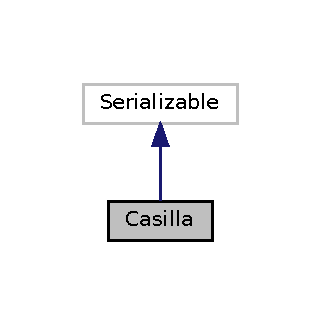
\includegraphics[width=154pt]{class_dominio_1_1clases_1_1_casilla__inherit__graph}
\end{center}
\end{figure}


Collaboration diagram for Casilla\+:
\nopagebreak
\begin{figure}[H]
\begin{center}
\leavevmode
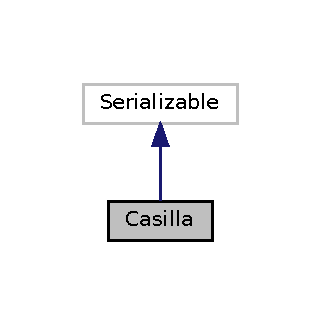
\includegraphics[width=154pt]{class_dominio_1_1clases_1_1_casilla__coll__graph}
\end{center}
\end{figure}
\subsection*{Data Structures}
\begin{DoxyCompactItemize}
\item 
enum {\bfseries Tipo}
\end{DoxyCompactItemize}
\subsection*{Public Member Functions}
\begin{DoxyCompactItemize}
\item 
\textbf{ Casilla} ()
\begin{DoxyCompactList}\small\item\em Inicializa los atributos de la casilla. \end{DoxyCompactList}\item 
\textbf{ Casilla} (\textbf{ Casilla} c)
\begin{DoxyCompactList}\small\item\em Inicializa los atributos de esta casilla con los atributos de la casilla pasada como parametro. \end{DoxyCompactList}\item 
\textbf{ Casilla} (boolean t, boolean h, boolean v, int val, int val\+Aux)
\begin{DoxyCompactList}\small\item\em Inicializa los atributos de esta casilla con los atributos pasados como parametro. \end{DoxyCompactList}\item 
void \textbf{ set\+Tipo} (boolean t)
\begin{DoxyCompactList}\small\item\em Modifica el tipo de la casilla. \end{DoxyCompactList}\item 
void \textbf{ set\+Horizontal} (boolean h)
\begin{DoxyCompactList}\small\item\em Modifica el booleano horizontal de la casilla. \end{DoxyCompactList}\item 
void \textbf{ set\+Vertical} (boolean v)
\begin{DoxyCompactList}\small\item\em Modifica el booleano vertical de la casilla. \end{DoxyCompactList}\item 
void \textbf{ set\+Valor} (int val)
\begin{DoxyCompactList}\small\item\em Modifica el valor de la casilla. \end{DoxyCompactList}\item 
void \textbf{ set\+Valor\+Aux} (int val)
\begin{DoxyCompactList}\small\item\em Modifica el valor auxiliar de la casilla. \end{DoxyCompactList}\item 
void \textbf{ setX} (int x)
\begin{DoxyCompactList}\small\item\em Modifica el atributo X de la casilla. \end{DoxyCompactList}\item 
void \textbf{ setY} (int y)
\begin{DoxyCompactList}\small\item\em Modifica el atributo Y de la casilla. \end{DoxyCompactList}\item 
boolean \textbf{ get\+Tipo} ()
\begin{DoxyCompactList}\small\item\em Consultora del tipo de la casilla. \end{DoxyCompactList}\item 
int \textbf{ get\+Valor} ()
\begin{DoxyCompactList}\small\item\em Consultora del valor de la casilla. \end{DoxyCompactList}\item 
int \textbf{ get\+Valor\+Aux} ()
\begin{DoxyCompactList}\small\item\em Consultora del valor auxiliar de la casilla. \end{DoxyCompactList}\item 
boolean \textbf{ get\+Horizontal} ()
\begin{DoxyCompactList}\small\item\em Consultora del valor horizontal de la casilla. \end{DoxyCompactList}\item 
boolean \textbf{ get\+Vertical} ()
\begin{DoxyCompactList}\small\item\em Consultora del valor vertical de la casilla. \end{DoxyCompactList}\item 
int \textbf{ getY} ()
\begin{DoxyCompactList}\small\item\em Consultora del valor Y de la casilla. \end{DoxyCompactList}\item 
int \textbf{ getX} ()
\begin{DoxyCompactList}\small\item\em Consultora del valor X de la casilla. \end{DoxyCompactList}\item 
String \textbf{ to\+String} ()
\begin{DoxyCompactList}\small\item\em Transforma la casilla al formato del kakuro. \end{DoxyCompactList}\item 
\mbox{\label{class_dominio_1_1clases_1_1_casilla_a36f9d82eba263d6a45140376547ca204}} 
\textbf{ Casilla} {\bfseries from\+String} (String cell)
\end{DoxyCompactItemize}


\subsection{Detailed Description}
Clase que representa una \doxyref{Casilla}{p.}{class_dominio_1_1clases_1_1_casilla} de un tablero de un \doxyref{Kakuro}{p.}{class_dominio_1_1clases_1_1_kakuro}. 

Definition at line 23 of file Casilla.\+java.



\subsection{Constructor \& Destructor Documentation}
\mbox{\label{class_dominio_1_1clases_1_1_casilla_aa4cf4820a1813678fb1900d88331171f}} 
\index{Dominio\+::clases\+::\+Casilla@{Dominio\+::clases\+::\+Casilla}!Casilla@{Casilla}}
\index{Casilla@{Casilla}!Dominio\+::clases\+::\+Casilla@{Dominio\+::clases\+::\+Casilla}}
\subsubsection{Casilla()\hspace{0.1cm}{\footnotesize\ttfamily [1/3]}}
{\footnotesize\ttfamily \textbf{ Casilla} (\begin{DoxyParamCaption}{ }\end{DoxyParamCaption})\hspace{0.3cm}{\ttfamily [inline]}}



Inicializa los atributos de la casilla. 

\begin{DoxyPostcond}{Postcondition}
tipo=Blanca, horizontal y vertical = false, valor y valor\+Aux = 0. 
\end{DoxyPostcond}


Definition at line 42 of file Casilla.\+java.

\mbox{\label{class_dominio_1_1clases_1_1_casilla_a2e4c39cd56901d7e8253d11e02d7d911}} 
\index{Dominio\+::clases\+::\+Casilla@{Dominio\+::clases\+::\+Casilla}!Casilla@{Casilla}}
\index{Casilla@{Casilla}!Dominio\+::clases\+::\+Casilla@{Dominio\+::clases\+::\+Casilla}}
\subsubsection{Casilla()\hspace{0.1cm}{\footnotesize\ttfamily [2/3]}}
{\footnotesize\ttfamily \textbf{ Casilla} (\begin{DoxyParamCaption}\item[{\textbf{ Casilla}}]{c }\end{DoxyParamCaption})\hspace{0.3cm}{\ttfamily [inline]}}



Inicializa los atributos de esta casilla con los atributos de la casilla pasada como parametro. 


\begin{DoxyParams}{Parameters}
{\em c} & = Una casilla no nula \\
\hline
\end{DoxyParams}
\begin{DoxyPostcond}{Postcondition}
La casilla actual es una copia de la casilla pasada como parametro 
\end{DoxyPostcond}


Definition at line 54 of file Casilla.\+java.

\mbox{\label{class_dominio_1_1clases_1_1_casilla_a6672cb0d1efd09434610eb26ddd38c58}} 
\index{Dominio\+::clases\+::\+Casilla@{Dominio\+::clases\+::\+Casilla}!Casilla@{Casilla}}
\index{Casilla@{Casilla}!Dominio\+::clases\+::\+Casilla@{Dominio\+::clases\+::\+Casilla}}
\subsubsection{Casilla()\hspace{0.1cm}{\footnotesize\ttfamily [3/3]}}
{\footnotesize\ttfamily \textbf{ Casilla} (\begin{DoxyParamCaption}\item[{boolean}]{t,  }\item[{boolean}]{h,  }\item[{boolean}]{v,  }\item[{int}]{val,  }\item[{int}]{val\+Aux }\end{DoxyParamCaption})\hspace{0.3cm}{\ttfamily [inline]}}



Inicializa los atributos de esta casilla con los atributos pasados como parametro. 


\begin{DoxyParams}{Parameters}
{\em t} & = true si la casilla es blanca o falso si es negra. \\
\hline
{\em h} & = indica si la casilla es horizontal. \\
\hline
{\em v} & = indica si la casilla es vertical. \\
\hline
{\em val} & = Indica el valor de la casilla. \\
\hline
{\em val\+Aux} & = Indica el valor auxiliar de la casilla. \\
\hline
\end{DoxyParams}
\begin{DoxyPostcond}{Postcondition}
Los atributos de esta casilla son iguales a los atributos pasados como parametro. 
\end{DoxyPostcond}


Definition at line 73 of file Casilla.\+java.



\subsection{Member Function Documentation}
\mbox{\label{class_dominio_1_1clases_1_1_casilla_a26ece4b98497f730b8c5d644b2c463c8}} 
\index{Dominio\+::clases\+::\+Casilla@{Dominio\+::clases\+::\+Casilla}!get\+Horizontal@{get\+Horizontal}}
\index{get\+Horizontal@{get\+Horizontal}!Dominio\+::clases\+::\+Casilla@{Dominio\+::clases\+::\+Casilla}}
\subsubsection{get\+Horizontal()}
{\footnotesize\ttfamily boolean get\+Horizontal (\begin{DoxyParamCaption}{ }\end{DoxyParamCaption})\hspace{0.3cm}{\ttfamily [inline]}}



Consultora del valor horizontal de la casilla. 

\begin{DoxyPostcond}{Postcondition}
Retorna si la casilla es horizontal o no. 
\end{DoxyPostcond}


Definition at line 145 of file Casilla.\+java.

\mbox{\label{class_dominio_1_1clases_1_1_casilla_ad03300c6376c01027c7e7693a2dd2279}} 
\index{Dominio\+::clases\+::\+Casilla@{Dominio\+::clases\+::\+Casilla}!get\+Tipo@{get\+Tipo}}
\index{get\+Tipo@{get\+Tipo}!Dominio\+::clases\+::\+Casilla@{Dominio\+::clases\+::\+Casilla}}
\subsubsection{get\+Tipo()}
{\footnotesize\ttfamily boolean get\+Tipo (\begin{DoxyParamCaption}{ }\end{DoxyParamCaption})\hspace{0.3cm}{\ttfamily [inline]}}



Consultora del tipo de la casilla. 

\begin{DoxyPostcond}{Postcondition}
Retorna true si la casilla es blanca y false si es negra. 
\end{DoxyPostcond}


Definition at line 130 of file Casilla.\+java.

\mbox{\label{class_dominio_1_1clases_1_1_casilla_ae8d545168f15c7f478e1fd3d4673622b}} 
\index{Dominio\+::clases\+::\+Casilla@{Dominio\+::clases\+::\+Casilla}!get\+Valor@{get\+Valor}}
\index{get\+Valor@{get\+Valor}!Dominio\+::clases\+::\+Casilla@{Dominio\+::clases\+::\+Casilla}}
\subsubsection{get\+Valor()}
{\footnotesize\ttfamily int get\+Valor (\begin{DoxyParamCaption}{ }\end{DoxyParamCaption})\hspace{0.3cm}{\ttfamily [inline]}}



Consultora del valor de la casilla. 

\begin{DoxyPostcond}{Postcondition}
Retorna el valor de la casilla. 
\end{DoxyPostcond}


Definition at line 135 of file Casilla.\+java.

\mbox{\label{class_dominio_1_1clases_1_1_casilla_a1456d9e36a115ef665a8b8f97f232244}} 
\index{Dominio\+::clases\+::\+Casilla@{Dominio\+::clases\+::\+Casilla}!get\+Valor\+Aux@{get\+Valor\+Aux}}
\index{get\+Valor\+Aux@{get\+Valor\+Aux}!Dominio\+::clases\+::\+Casilla@{Dominio\+::clases\+::\+Casilla}}
\subsubsection{get\+Valor\+Aux()}
{\footnotesize\ttfamily int get\+Valor\+Aux (\begin{DoxyParamCaption}{ }\end{DoxyParamCaption})\hspace{0.3cm}{\ttfamily [inline]}}



Consultora del valor auxiliar de la casilla. 

\begin{DoxyPostcond}{Postcondition}
Retorna el valor auxiliar de la casilla. 
\end{DoxyPostcond}


Definition at line 140 of file Casilla.\+java.

\mbox{\label{class_dominio_1_1clases_1_1_casilla_a27c6abc4a3d15d86c82f7ffabca42650}} 
\index{Dominio\+::clases\+::\+Casilla@{Dominio\+::clases\+::\+Casilla}!get\+Vertical@{get\+Vertical}}
\index{get\+Vertical@{get\+Vertical}!Dominio\+::clases\+::\+Casilla@{Dominio\+::clases\+::\+Casilla}}
\subsubsection{get\+Vertical()}
{\footnotesize\ttfamily boolean get\+Vertical (\begin{DoxyParamCaption}{ }\end{DoxyParamCaption})\hspace{0.3cm}{\ttfamily [inline]}}



Consultora del valor vertical de la casilla. 

\begin{DoxyPostcond}{Postcondition}
Retorna si la casilla es vertical o no. 
\end{DoxyPostcond}


Definition at line 150 of file Casilla.\+java.

\mbox{\label{class_dominio_1_1clases_1_1_casilla_ae13f88e922e1339355456062ad9fa359}} 
\index{Dominio\+::clases\+::\+Casilla@{Dominio\+::clases\+::\+Casilla}!getX@{getX}}
\index{getX@{getX}!Dominio\+::clases\+::\+Casilla@{Dominio\+::clases\+::\+Casilla}}
\subsubsection{get\+X()}
{\footnotesize\ttfamily int getX (\begin{DoxyParamCaption}{ }\end{DoxyParamCaption})\hspace{0.3cm}{\ttfamily [inline]}}



Consultora del valor X de la casilla. 

\begin{DoxyPostcond}{Postcondition}
Retorna el atributo X de la casilla. 
\end{DoxyPostcond}


Definition at line 160 of file Casilla.\+java.

\mbox{\label{class_dominio_1_1clases_1_1_casilla_aab81944f0a14bba932c0931899951937}} 
\index{Dominio\+::clases\+::\+Casilla@{Dominio\+::clases\+::\+Casilla}!getY@{getY}}
\index{getY@{getY}!Dominio\+::clases\+::\+Casilla@{Dominio\+::clases\+::\+Casilla}}
\subsubsection{get\+Y()}
{\footnotesize\ttfamily int getY (\begin{DoxyParamCaption}{ }\end{DoxyParamCaption})\hspace{0.3cm}{\ttfamily [inline]}}



Consultora del valor Y de la casilla. 

\begin{DoxyPostcond}{Postcondition}
Retorna el atributo Y de la casilla. 
\end{DoxyPostcond}


Definition at line 155 of file Casilla.\+java.

\mbox{\label{class_dominio_1_1clases_1_1_casilla_aa13c72fa2f4ed3ee3abc1fa8fbb375d3}} 
\index{Dominio\+::clases\+::\+Casilla@{Dominio\+::clases\+::\+Casilla}!set\+Horizontal@{set\+Horizontal}}
\index{set\+Horizontal@{set\+Horizontal}!Dominio\+::clases\+::\+Casilla@{Dominio\+::clases\+::\+Casilla}}
\subsubsection{set\+Horizontal()}
{\footnotesize\ttfamily void set\+Horizontal (\begin{DoxyParamCaption}\item[{boolean}]{h }\end{DoxyParamCaption})\hspace{0.3cm}{\ttfamily [inline]}}



Modifica el booleano horizontal de la casilla. 


\begin{DoxyParams}{Parameters}
{\em h} & = indica si la casilla es horizontal o no. \\
\hline
\end{DoxyParams}
\begin{DoxyPostcond}{Postcondition}
La casilla modifica el booleano horizontal de acuerdo al parametro pasado. 
\end{DoxyPostcond}


Definition at line 93 of file Casilla.\+java.

\mbox{\label{class_dominio_1_1clases_1_1_casilla_ad835c28dba2b7ebbf9c95fd81a3700ca}} 
\index{Dominio\+::clases\+::\+Casilla@{Dominio\+::clases\+::\+Casilla}!set\+Tipo@{set\+Tipo}}
\index{set\+Tipo@{set\+Tipo}!Dominio\+::clases\+::\+Casilla@{Dominio\+::clases\+::\+Casilla}}
\subsubsection{set\+Tipo()}
{\footnotesize\ttfamily void set\+Tipo (\begin{DoxyParamCaption}\item[{boolean}]{t }\end{DoxyParamCaption})\hspace{0.3cm}{\ttfamily [inline]}}



Modifica el tipo de la casilla. 


\begin{DoxyParams}{Parameters}
{\em t} & = true indica que la casilla es blanca y false que es negra. \\
\hline
\end{DoxyParams}
\begin{DoxyPostcond}{Postcondition}
La casilla modifica el tipo de acuerdo al parametro pasado. 
\end{DoxyPostcond}


Definition at line 87 of file Casilla.\+java.

\mbox{\label{class_dominio_1_1clases_1_1_casilla_a9f88bf1a462e0301c0a78e3c40baaa91}} 
\index{Dominio\+::clases\+::\+Casilla@{Dominio\+::clases\+::\+Casilla}!set\+Valor@{set\+Valor}}
\index{set\+Valor@{set\+Valor}!Dominio\+::clases\+::\+Casilla@{Dominio\+::clases\+::\+Casilla}}
\subsubsection{set\+Valor()}
{\footnotesize\ttfamily void set\+Valor (\begin{DoxyParamCaption}\item[{int}]{val }\end{DoxyParamCaption})\hspace{0.3cm}{\ttfamily [inline]}}



Modifica el valor de la casilla. 


\begin{DoxyParams}{Parameters}
{\em val} & = indica el nuevo valor de la casilla. \\
\hline
\end{DoxyParams}
\begin{DoxyPostcond}{Postcondition}
La casilla modifica el valor de acuerdo al parametro pasado. 
\end{DoxyPostcond}


Definition at line 105 of file Casilla.\+java.

\mbox{\label{class_dominio_1_1clases_1_1_casilla_a57cc2f2b320fee75228671b47bd2c6c9}} 
\index{Dominio\+::clases\+::\+Casilla@{Dominio\+::clases\+::\+Casilla}!set\+Valor\+Aux@{set\+Valor\+Aux}}
\index{set\+Valor\+Aux@{set\+Valor\+Aux}!Dominio\+::clases\+::\+Casilla@{Dominio\+::clases\+::\+Casilla}}
\subsubsection{set\+Valor\+Aux()}
{\footnotesize\ttfamily void set\+Valor\+Aux (\begin{DoxyParamCaption}\item[{int}]{val }\end{DoxyParamCaption})\hspace{0.3cm}{\ttfamily [inline]}}



Modifica el valor auxiliar de la casilla. 


\begin{DoxyParams}{Parameters}
{\em val} & = indica el nuevo valor auxiliar de la casilla. \\
\hline
\end{DoxyParams}
\begin{DoxyPostcond}{Postcondition}
La casilla modifica el valor auxiliar de acuerdo al parametro pasado. 
\end{DoxyPostcond}


Definition at line 111 of file Casilla.\+java.

\mbox{\label{class_dominio_1_1clases_1_1_casilla_a1c8dfaea880d06c914d02858a3d9a8c2}} 
\index{Dominio\+::clases\+::\+Casilla@{Dominio\+::clases\+::\+Casilla}!set\+Vertical@{set\+Vertical}}
\index{set\+Vertical@{set\+Vertical}!Dominio\+::clases\+::\+Casilla@{Dominio\+::clases\+::\+Casilla}}
\subsubsection{set\+Vertical()}
{\footnotesize\ttfamily void set\+Vertical (\begin{DoxyParamCaption}\item[{boolean}]{v }\end{DoxyParamCaption})\hspace{0.3cm}{\ttfamily [inline]}}



Modifica el booleano vertical de la casilla. 


\begin{DoxyParams}{Parameters}
{\em v} & = indica si la casilla es vertical o no. \\
\hline
\end{DoxyParams}
\begin{DoxyPostcond}{Postcondition}
La casilla modifica el booleano vertical de acuerdo al parametro pasado. 
\end{DoxyPostcond}


Definition at line 99 of file Casilla.\+java.

\mbox{\label{class_dominio_1_1clases_1_1_casilla_add2578ea6b65ad27a905a6d2048748bb}} 
\index{Dominio\+::clases\+::\+Casilla@{Dominio\+::clases\+::\+Casilla}!setX@{setX}}
\index{setX@{setX}!Dominio\+::clases\+::\+Casilla@{Dominio\+::clases\+::\+Casilla}}
\subsubsection{set\+X()}
{\footnotesize\ttfamily void setX (\begin{DoxyParamCaption}\item[{int}]{x }\end{DoxyParamCaption})\hspace{0.3cm}{\ttfamily [inline]}}



Modifica el atributo X de la casilla. 


\begin{DoxyParams}{Parameters}
{\em x} & = indica el nuevo valor de X de la casilla. \\
\hline
\end{DoxyParams}
\begin{DoxyPostcond}{Postcondition}
La casilla modifica el valor de X de acuerdo al parametro pasado. 
\end{DoxyPostcond}


Definition at line 117 of file Casilla.\+java.

\mbox{\label{class_dominio_1_1clases_1_1_casilla_adea78a9ff1234e75627dda61d972213b}} 
\index{Dominio\+::clases\+::\+Casilla@{Dominio\+::clases\+::\+Casilla}!setY@{setY}}
\index{setY@{setY}!Dominio\+::clases\+::\+Casilla@{Dominio\+::clases\+::\+Casilla}}
\subsubsection{set\+Y()}
{\footnotesize\ttfamily void setY (\begin{DoxyParamCaption}\item[{int}]{y }\end{DoxyParamCaption})\hspace{0.3cm}{\ttfamily [inline]}}



Modifica el atributo Y de la casilla. 


\begin{DoxyParams}{Parameters}
{\em y} & = indica el nuevo valor de Y de la casilla. \\
\hline
\end{DoxyParams}
\begin{DoxyPostcond}{Postcondition}
La casilla modifica el valor de Y de acuerdo al parametro pasado. 
\end{DoxyPostcond}


Definition at line 123 of file Casilla.\+java.

\mbox{\label{class_dominio_1_1clases_1_1_casilla_ad146fa8579a5f8a876c4688cc5a68520}} 
\index{Dominio\+::clases\+::\+Casilla@{Dominio\+::clases\+::\+Casilla}!to\+String@{to\+String}}
\index{to\+String@{to\+String}!Dominio\+::clases\+::\+Casilla@{Dominio\+::clases\+::\+Casilla}}
\subsubsection{to\+String()}
{\footnotesize\ttfamily String to\+String (\begin{DoxyParamCaption}{ }\end{DoxyParamCaption})\hspace{0.3cm}{\ttfamily [inline]}}



Transforma la casilla al formato del kakuro. 

\begin{DoxyPostcond}{Postcondition}
Retorna un string con los datos de la casilla transformados al formato del \doxyref{Kakuro}{p.}{class_dominio_1_1clases_1_1_kakuro}. 
\end{DoxyPostcond}


Definition at line 166 of file Casilla.\+java.



The documentation for this class was generated from the following file\+:\begin{DoxyCompactItemize}
\item 
src/\+Dominio/clases/\textbf{ Casilla.\+java}\end{DoxyCompactItemize}

\section{Ctrl\+Capa\+Dominio Class Reference}
\label{class_dominio_1_1controladores_1_1_ctrl_capa_dominio}\index{Ctrl\+Capa\+Dominio@{Ctrl\+Capa\+Dominio}}


Clase que se utiliza como intermediaria entre presentacion y persistencia. Transforma los datos que recibe de persistencia y se los pasa a presentacion.  




Collaboration diagram for Ctrl\+Capa\+Dominio\+:
\nopagebreak
\begin{figure}[H]
\begin{center}
\leavevmode
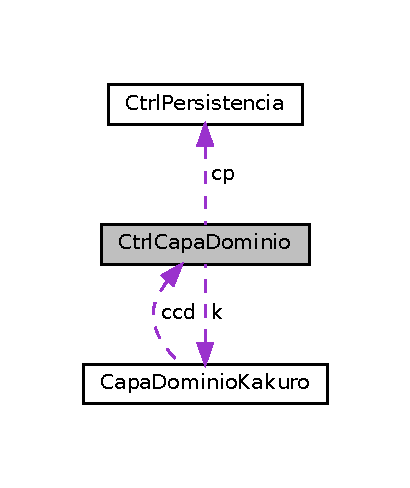
\includegraphics[width=197pt]{class_dominio_1_1controladores_1_1_ctrl_capa_dominio__coll__graph}
\end{center}
\end{figure}
\subsection*{Public Member Functions}
\begin{DoxyCompactItemize}
\item 
\textbf{ Ctrl\+Capa\+Dominio} ()
\begin{DoxyCompactList}\small\item\em Constructora de \doxyref{Ctrl\+Capa\+Dominio}{p.}{class_dominio_1_1controladores_1_1_ctrl_capa_dominio}. \end{DoxyCompactList}\item 
void \textbf{ anadir\+\_\+usuario} (String usuario, String password)
\begin{DoxyCompactList}\small\item\em Recibe los datos de un Usuario que debe mandar a persistencia y que esta se encargue de guardarlos. \end{DoxyCompactList}\item 
boolean \textbf{ comprobar} (int n, String Usuario, String Password)
\begin{DoxyCompactList}\small\item\em Comrpueba si el Usuario que pretende hacer inicio de sesion, ha introcucido sus datos correctamente. En el caso que quiera regsitrarse, comprobará que el nombre de Usuario que elija no exista. \end{DoxyCompactList}\item 
boolean \textbf{ Log\+In} (String User, char[$\,$] Pass)
\begin{DoxyCompactList}\small\item\em recibe un usuario password de la capa de presentacion y deberá comprobar si el login es correcto \end{DoxyCompactList}\item 
boolean \textbf{ Sign\+Up} (String User, char[$\,$] Pass)
\begin{DoxyCompactList}\small\item\em recibe un usuario password de la capa de presentacion y deberá comprobar si el registro será posible \end{DoxyCompactList}\item 
String [$\,$] \textbf{ Cargar\+I\+Ds} (String User)
\begin{DoxyCompactList}\small\item\em funcion que se encarga de buscar los ids de la partidas que tiene guardadas el usuario con nombre \char`\"{}\+User\char`\"{} que se pasa como parámetro \end{DoxyCompactList}\item 
boolean \textbf{ guardar\+\_\+partida} (String I\+D\+User, String I\+D\+Partida, String[$\,$][$\,$] tablero, int I\+D\+Kakuro, int tiempo, boolean finished)
\begin{DoxyCompactList}\small\item\em funcion que se encarga de recibir los datos de una partida en juego que se quiere guardar y almacenarlos \end{DoxyCompactList}\item 
String [$\,$][$\,$] \textbf{ cargar\+\_\+partida} (String User, String I\+D\+Partida)
\begin{DoxyCompactList}\small\item\em función que se encarga de buscar y transformar una partida solicitada por un usuario, para que se pueda retomar por donde la dejó \end{DoxyCompactList}\item 
String [$\,$] \textbf{ get\+\_\+lista\+\_\+kakuro} ()
\begin{DoxyCompactList}\small\item\em busca todos los Ids que hay almacenados en la Biblioteca de Kakuros \end{DoxyCompactList}\item 
String [$\,$][$\,$] \textbf{ Show\+Solution} (String ID)
\begin{DoxyCompactList}\small\item\em Calcula la solución del kakuro que está en juego. \end{DoxyCompactList}\item 
String \textbf{ Show\+Ranking} ()
\begin{DoxyCompactList}\small\item\em obtendra el ranking de jugadores \end{DoxyCompactList}\item 
void \textbf{ update\+Ranking} (String Key, double Value)
\begin{DoxyCompactList}\small\item\em se encarga de actulizar el ranking cuando se le pasa un jugador y una puntuacion. Si el usuario no habia terminado ninguna partid antes, se le añadirá nuevo. En otro caso se le actulizará la puntuación \end{DoxyCompactList}\item 
String [$\,$][$\,$] \textbf{ getkakuroenjuego} (int id)
\begin{DoxyCompactList}\small\item\em buscará el kakuro que tiene como identificador el id que se pasa como parámetro y lo teranformará a una matriz de String \end{DoxyCompactList}\item 
int \textbf{ generar\+Kakuro} (int dificultad)
\begin{DoxyCompactList}\small\item\em generará un kakuro con la dificultad indicada \end{DoxyCompactList}\item 
int \textbf{ generar\+Kakuro} (int dimensiones, int num\+Casillas\+Negras)
\item 
\mbox{\label{class_dominio_1_1controladores_1_1_ctrl_capa_dominio_a95df7bb86f38a4123b7caf44b60afef1}} 
String {\bfseries generar\+Kakuro\+Manual} (String[$\,$][$\,$] grid\+Contents\+Matrix)
\item 
int \textbf{ addkakuro} (\textbf{ Casilla}[$\,$][$\,$] tablero)
\begin{DoxyCompactList}\small\item\em se encarga de pasarle un kakuro a la capa de persistencia para que lo guarde \end{DoxyCompactList}\item 
\textbf{ Kakuro} \textbf{ read\+\_\+kakuro\+\_\+file} (int ID, int option)
\begin{DoxyCompactList}\small\item\em buscará un kakuro que tenga el id que se pasa como paramétro \end{DoxyCompactList}\item 
int \textbf{ comprobar\+Movimiento} (int x, int y, String value, String[$\,$][$\,$] grid\+Contents\+Matrix)
\begin{DoxyCompactList}\small\item\em se encarga de comprobar si el valor \char`\"{}value\char`\"{} en el kakuro recibido es valido en la posicion \char`\"{}x,y\char`\"{} \end{DoxyCompactList}\item 
int \textbf{ get\+Kakuro\+De\+Partida} (String I\+D\+Usuario, String I\+D\+Partida)
\begin{DoxyCompactList}\small\item\em se encarga de obtener, si existe, el kakuro del usuario I\+D\+Usuario identificado por I\+D\+Partida \end{DoxyCompactList}\item 
void \textbf{ set\+Map} ()
\begin{DoxyCompactList}\small\item\em llama a la funcion set\+Map de la clase Ctrl\+Persistencia pasandole el atributo listaP \end{DoxyCompactList}\item 
int \textbf{ get\+Time\+De\+Partida} (String I\+D\+Usuario, String I\+D\+Partida)
\begin{DoxyCompactList}\small\item\em obtiene el tiempo transcurrido de la partida identificada con \char`\"{}\+I\+D\+Partida\char`\"{} asociado al usuario \char`\"{}\+I\+D\+Usuario\char`\"{}(si existe) \end{DoxyCompactList}\end{DoxyCompactItemize}


\subsection{Detailed Description}
Clase que se utiliza como intermediaria entre presentacion y persistencia. Transforma los datos que recibe de persistencia y se los pasa a presentacion. 

Definition at line 37 of file Ctrl\+Capa\+Dominio.\+java.



\subsection{Constructor \& Destructor Documentation}
\mbox{\label{class_dominio_1_1controladores_1_1_ctrl_capa_dominio_a61d89e049d057d28ce0a8d9adbf45e90}} 
\index{Dominio\+::controladores\+::\+Ctrl\+Capa\+Dominio@{Dominio\+::controladores\+::\+Ctrl\+Capa\+Dominio}!Ctrl\+Capa\+Dominio@{Ctrl\+Capa\+Dominio}}
\index{Ctrl\+Capa\+Dominio@{Ctrl\+Capa\+Dominio}!Dominio\+::controladores\+::\+Ctrl\+Capa\+Dominio@{Dominio\+::controladores\+::\+Ctrl\+Capa\+Dominio}}
\subsubsection{Ctrl\+Capa\+Dominio()}
{\footnotesize\ttfamily \textbf{ Ctrl\+Capa\+Dominio} (\begin{DoxyParamCaption}{ }\end{DoxyParamCaption})\hspace{0.3cm}{\ttfamily [inline]}}



Constructora de \doxyref{Ctrl\+Capa\+Dominio}{p.}{class_dominio_1_1controladores_1_1_ctrl_capa_dominio}. 

\begin{DoxyPostcond}{Postcondition}
se crea una nueva instancia de \doxyref{Ctrl\+Capa\+Dominio}{p.}{class_dominio_1_1controladores_1_1_ctrl_capa_dominio} 
\end{DoxyPostcond}


Definition at line 49 of file Ctrl\+Capa\+Dominio.\+java.



\subsection{Member Function Documentation}
\mbox{\label{class_dominio_1_1controladores_1_1_ctrl_capa_dominio_a6953d179f5f27e8d94c6dfb6d9b1a663}} 
\index{Dominio\+::controladores\+::\+Ctrl\+Capa\+Dominio@{Dominio\+::controladores\+::\+Ctrl\+Capa\+Dominio}!addkakuro@{addkakuro}}
\index{addkakuro@{addkakuro}!Dominio\+::controladores\+::\+Ctrl\+Capa\+Dominio@{Dominio\+::controladores\+::\+Ctrl\+Capa\+Dominio}}
\subsubsection{addkakuro()}
{\footnotesize\ttfamily int addkakuro (\begin{DoxyParamCaption}\item[{\textbf{ Casilla}}]{tablero[$\,$][$\,$] }\end{DoxyParamCaption})\hspace{0.3cm}{\ttfamily [inline]}}



se encarga de pasarle un kakuro a la capa de persistencia para que lo guarde 


\begin{DoxyParams}{Parameters}
{\em tablero} & = matriz de casillas que representa el kakuro\\
\hline
\end{DoxyParams}
\begin{DoxyPostcond}{Postcondition}
devuelve un entero que representa el id que se la ha asignado al nuevo kakuro 
\end{DoxyPostcond}


Definition at line 566 of file Ctrl\+Capa\+Dominio.\+java.

\mbox{\label{class_dominio_1_1controladores_1_1_ctrl_capa_dominio_a5c5e5b25f6e13bcff9a5db7afd8798d3}} 
\index{Dominio\+::controladores\+::\+Ctrl\+Capa\+Dominio@{Dominio\+::controladores\+::\+Ctrl\+Capa\+Dominio}!anadir\+\_\+usuario@{anadir\+\_\+usuario}}
\index{anadir\+\_\+usuario@{anadir\+\_\+usuario}!Dominio\+::controladores\+::\+Ctrl\+Capa\+Dominio@{Dominio\+::controladores\+::\+Ctrl\+Capa\+Dominio}}
\subsubsection{anadir\+\_\+usuario()}
{\footnotesize\ttfamily void anadir\+\_\+usuario (\begin{DoxyParamCaption}\item[{String}]{usuario,  }\item[{String}]{password }\end{DoxyParamCaption})\hspace{0.3cm}{\ttfamily [inline]}}



Recibe los datos de un Usuario que debe mandar a persistencia y que esta se encargue de guardarlos. 


\begin{DoxyParams}{Parameters}
{\em Usuario} & = Es el nombre de usuario que ha elegido para el registro \\
\hline
{\em Password} & = Es la contraseña que el usuario ha elegido para el registro\\
\hline
\end{DoxyParams}
\begin{DoxyPostcond}{Postcondition}
Se ha guaradado un nuevo Usuario con \char`\"{}\+Usuario\char`\"{} y \char`\"{}\+Password\char`\"{} 
\end{DoxyPostcond}


Definition at line 71 of file Ctrl\+Capa\+Dominio.\+java.

\mbox{\label{class_dominio_1_1controladores_1_1_ctrl_capa_dominio_ab6c07eaf528a5ad487369a7561766057}} 
\index{Dominio\+::controladores\+::\+Ctrl\+Capa\+Dominio@{Dominio\+::controladores\+::\+Ctrl\+Capa\+Dominio}!cargar\+\_\+partida@{cargar\+\_\+partida}}
\index{cargar\+\_\+partida@{cargar\+\_\+partida}!Dominio\+::controladores\+::\+Ctrl\+Capa\+Dominio@{Dominio\+::controladores\+::\+Ctrl\+Capa\+Dominio}}
\subsubsection{cargar\+\_\+partida()}
{\footnotesize\ttfamily String [$\,$][$\,$] cargar\+\_\+partida (\begin{DoxyParamCaption}\item[{String}]{User,  }\item[{String}]{I\+D\+Partida }\end{DoxyParamCaption})\hspace{0.3cm}{\ttfamily [inline]}}



función que se encarga de buscar y transformar una partida solicitada por un usuario, para que se pueda retomar por donde la dejó 


\begin{DoxyParams}{Parameters}
{\em User} & = nombre de usuario del jugador \\
\hline
{\em I\+D\+Partida} & = nombre con el cual guardó la partida anteriormente\\
\hline
\end{DoxyParams}
\begin{DoxyPostcond}{Postcondition}
Se devuelve una matriz de Strning la cual contiene el tablero del kakuro tal y como se quedó la ultima vez que jugó 
\end{DoxyPostcond}


Definition at line 297 of file Ctrl\+Capa\+Dominio.\+java.

\mbox{\label{class_dominio_1_1controladores_1_1_ctrl_capa_dominio_a1da2be254d68f7c913ca7b872ffa3af2}} 
\index{Dominio\+::controladores\+::\+Ctrl\+Capa\+Dominio@{Dominio\+::controladores\+::\+Ctrl\+Capa\+Dominio}!Cargar\+I\+Ds@{Cargar\+I\+Ds}}
\index{Cargar\+I\+Ds@{Cargar\+I\+Ds}!Dominio\+::controladores\+::\+Ctrl\+Capa\+Dominio@{Dominio\+::controladores\+::\+Ctrl\+Capa\+Dominio}}
\subsubsection{Cargar\+I\+Ds()}
{\footnotesize\ttfamily String [$\,$] Cargar\+I\+Ds (\begin{DoxyParamCaption}\item[{String}]{User }\end{DoxyParamCaption})\hspace{0.3cm}{\ttfamily [inline]}}



funcion que se encarga de buscar los ids de la partidas que tiene guardadas el usuario con nombre \char`\"{}\+User\char`\"{} que se pasa como parámetro 


\begin{DoxyParams}{Parameters}
{\em User} & = nombre de Usuario para el cual se quiere buscar las partidas guardadas\\
\hline
\end{DoxyParams}
\begin{DoxyPostcond}{Postcondition}
se devuelve un vector de Strings con los nombres de sus partidas 
\end{DoxyPostcond}


Definition at line 169 of file Ctrl\+Capa\+Dominio.\+java.

\mbox{\label{class_dominio_1_1controladores_1_1_ctrl_capa_dominio_a1e108c711ab803c873740074187ffc25}} 
\index{Dominio\+::controladores\+::\+Ctrl\+Capa\+Dominio@{Dominio\+::controladores\+::\+Ctrl\+Capa\+Dominio}!comprobar@{comprobar}}
\index{comprobar@{comprobar}!Dominio\+::controladores\+::\+Ctrl\+Capa\+Dominio@{Dominio\+::controladores\+::\+Ctrl\+Capa\+Dominio}}
\subsubsection{comprobar()}
{\footnotesize\ttfamily boolean comprobar (\begin{DoxyParamCaption}\item[{int}]{n,  }\item[{String}]{Usuario,  }\item[{String}]{Password }\end{DoxyParamCaption})\hspace{0.3cm}{\ttfamily [inline]}}



Comrpueba si el Usuario que pretende hacer inicio de sesion, ha introcucido sus datos correctamente. En el caso que quiera regsitrarse, comprobará que el nombre de Usuario que elija no exista. 


\begin{DoxyParams}{Parameters}
{\em n} & = Parámetro que determina si hara una funcionalidad u otra. \\
\hline
{\em Usuario} & = Es el nombre de usuario que ha elegido para el registro o con el que quiere iniciar sesion \\
\hline
{\em Password} & = Es la contraseña que el usuario ha elegido para el registro o con la que quiere iniciar sesion\\
\hline
\end{DoxyParams}
\begin{DoxyPostcond}{Postcondition}
Devuelve un booleano que indicará al sistema lo que debe hacer segun lo que ha pedido el usuario 
\end{DoxyPostcond}


Definition at line 92 of file Ctrl\+Capa\+Dominio.\+java.

\mbox{\label{class_dominio_1_1controladores_1_1_ctrl_capa_dominio_a6f44b9ac88eba045ce4c5ad6bb03e435}} 
\index{Dominio\+::controladores\+::\+Ctrl\+Capa\+Dominio@{Dominio\+::controladores\+::\+Ctrl\+Capa\+Dominio}!comprobar\+Movimiento@{comprobar\+Movimiento}}
\index{comprobar\+Movimiento@{comprobar\+Movimiento}!Dominio\+::controladores\+::\+Ctrl\+Capa\+Dominio@{Dominio\+::controladores\+::\+Ctrl\+Capa\+Dominio}}
\subsubsection{comprobar\+Movimiento()}
{\footnotesize\ttfamily int comprobar\+Movimiento (\begin{DoxyParamCaption}\item[{int}]{x,  }\item[{int}]{y,  }\item[{String}]{value,  }\item[{String}]{grid\+Contents\+Matrix[$\,$][$\,$] }\end{DoxyParamCaption})\hspace{0.3cm}{\ttfamily [inline]}}



se encarga de comprobar si el valor \char`\"{}value\char`\"{} en el kakuro recibido es valido en la posicion \char`\"{}x,y\char`\"{} 


\begin{DoxyParams}{Parameters}
{\em x} & = valor de la posicion modificada en el eje x \\
\hline
{\em y} & = valor de la posicion modificada en el eje y \\
\hline
{\em value} & = valor modificado \\
\hline
{\em grid\+Contents\+Matrix} & = tablero sobre el cual se hizo la modificacion\\
\hline
\end{DoxyParams}
\begin{DoxyPostcond}{Postcondition}
se ha devuelto el resultado de llamar a la funcion con el mismo nombre de la clase Kakuro. 
\end{DoxyPostcond}


Definition at line 598 of file Ctrl\+Capa\+Dominio.\+java.

\mbox{\label{class_dominio_1_1controladores_1_1_ctrl_capa_dominio_a4e42ae85a1df8f7e0c667ab371e0a6f5}} 
\index{Dominio\+::controladores\+::\+Ctrl\+Capa\+Dominio@{Dominio\+::controladores\+::\+Ctrl\+Capa\+Dominio}!generar\+Kakuro@{generar\+Kakuro}}
\index{generar\+Kakuro@{generar\+Kakuro}!Dominio\+::controladores\+::\+Ctrl\+Capa\+Dominio@{Dominio\+::controladores\+::\+Ctrl\+Capa\+Dominio}}
\subsubsection{generar\+Kakuro()\hspace{0.1cm}{\footnotesize\ttfamily [1/2]}}
{\footnotesize\ttfamily int generar\+Kakuro (\begin{DoxyParamCaption}\item[{int}]{dificultad }\end{DoxyParamCaption})\hspace{0.3cm}{\ttfamily [inline]}}



generará un kakuro con la dificultad indicada 


\begin{DoxyParams}{Parameters}
{\em dificultad} & = es la dificultad con la que se generará el kakuro\\
\hline
\end{DoxyParams}
\begin{DoxyPostcond}{Postcondition}
devolverá un entero que representa el id que tiene el nuevo kakuro que se ha generado 
\end{DoxyPostcond}


Definition at line 517 of file Ctrl\+Capa\+Dominio.\+java.

\mbox{\label{class_dominio_1_1controladores_1_1_ctrl_capa_dominio_a67572196715612e05554990a74b06bf4}} 
\index{Dominio\+::controladores\+::\+Ctrl\+Capa\+Dominio@{Dominio\+::controladores\+::\+Ctrl\+Capa\+Dominio}!generar\+Kakuro@{generar\+Kakuro}}
\index{generar\+Kakuro@{generar\+Kakuro}!Dominio\+::controladores\+::\+Ctrl\+Capa\+Dominio@{Dominio\+::controladores\+::\+Ctrl\+Capa\+Dominio}}
\subsubsection{generar\+Kakuro()\hspace{0.1cm}{\footnotesize\ttfamily [2/2]}}
{\footnotesize\ttfamily int generar\+Kakuro (\begin{DoxyParamCaption}\item[{int}]{dimensiones,  }\item[{int}]{num\+Casillas\+Negras }\end{DoxyParamCaption})\hspace{0.3cm}{\ttfamily [inline]}}

generará un kakuro con las caracteristicas que se pasan como parámetros


\begin{DoxyParams}{Parameters}
{\em dimensiones} & = dimensiones con las cuales se generará el kakuro \\
\hline
{\em num\+Casillas\+Negras} & = numero de casillas negras que tendrá el kakuro\\
\hline
\end{DoxyParams}
\begin{DoxyPostcond}{Postcondition}
devolverá un entero que representa el id que tiene el nuevo kakuro que se ha generado 
\end{DoxyPostcond}


Definition at line 530 of file Ctrl\+Capa\+Dominio.\+java.

\mbox{\label{class_dominio_1_1controladores_1_1_ctrl_capa_dominio_a45ebd0e10cf0731cbd580006a2b9e365}} 
\index{Dominio\+::controladores\+::\+Ctrl\+Capa\+Dominio@{Dominio\+::controladores\+::\+Ctrl\+Capa\+Dominio}!get\+\_\+lista\+\_\+kakuro@{get\+\_\+lista\+\_\+kakuro}}
\index{get\+\_\+lista\+\_\+kakuro@{get\+\_\+lista\+\_\+kakuro}!Dominio\+::controladores\+::\+Ctrl\+Capa\+Dominio@{Dominio\+::controladores\+::\+Ctrl\+Capa\+Dominio}}
\subsubsection{get\+\_\+lista\+\_\+kakuro()}
{\footnotesize\ttfamily String [$\,$] get\+\_\+lista\+\_\+kakuro (\begin{DoxyParamCaption}{ }\end{DoxyParamCaption})\hspace{0.3cm}{\ttfamily [inline]}}



busca todos los Ids que hay almacenados en la Biblioteca de Kakuros 

\begin{DoxyPostcond}{Postcondition}
devuelve un vector de Strings con los I\+Ds de los Kakuro existentes en la biblioteca 
\end{DoxyPostcond}


Definition at line 391 of file Ctrl\+Capa\+Dominio.\+java.

\mbox{\label{class_dominio_1_1controladores_1_1_ctrl_capa_dominio_a14997dd10ecf7cf3cc5fbf85517abc65}} 
\index{Dominio\+::controladores\+::\+Ctrl\+Capa\+Dominio@{Dominio\+::controladores\+::\+Ctrl\+Capa\+Dominio}!get\+Kakuro\+De\+Partida@{get\+Kakuro\+De\+Partida}}
\index{get\+Kakuro\+De\+Partida@{get\+Kakuro\+De\+Partida}!Dominio\+::controladores\+::\+Ctrl\+Capa\+Dominio@{Dominio\+::controladores\+::\+Ctrl\+Capa\+Dominio}}
\subsubsection{get\+Kakuro\+De\+Partida()}
{\footnotesize\ttfamily int get\+Kakuro\+De\+Partida (\begin{DoxyParamCaption}\item[{String}]{I\+D\+Usuario,  }\item[{String}]{I\+D\+Partida }\end{DoxyParamCaption})\hspace{0.3cm}{\ttfamily [inline]}}



se encarga de obtener, si existe, el kakuro del usuario I\+D\+Usuario identificado por I\+D\+Partida 


\begin{DoxyParams}{Parameters}
{\em I\+D\+Usuario} & = identificador del usuario \\
\hline
{\em I\+D\+Partida} & = identificador de la partida\\
\hline
\end{DoxyParams}
\begin{DoxyPostcond}{Postcondition}
si se ha encontrado el Kakuro solicitado lo devuelve. En caso contrario devuelve -\/1 
\end{DoxyPostcond}


Definition at line 622 of file Ctrl\+Capa\+Dominio.\+java.

\mbox{\label{class_dominio_1_1controladores_1_1_ctrl_capa_dominio_a6a6d6fda88d7f224cac678d508f5c2a2}} 
\index{Dominio\+::controladores\+::\+Ctrl\+Capa\+Dominio@{Dominio\+::controladores\+::\+Ctrl\+Capa\+Dominio}!getkakuroenjuego@{getkakuroenjuego}}
\index{getkakuroenjuego@{getkakuroenjuego}!Dominio\+::controladores\+::\+Ctrl\+Capa\+Dominio@{Dominio\+::controladores\+::\+Ctrl\+Capa\+Dominio}}
\subsubsection{getkakuroenjuego()}
{\footnotesize\ttfamily String [$\,$][$\,$] getkakuroenjuego (\begin{DoxyParamCaption}\item[{int}]{id }\end{DoxyParamCaption})\hspace{0.3cm}{\ttfamily [inline]}}



buscará el kakuro que tiene como identificador el id que se pasa como parámetro y lo teranformará a una matriz de String 


\begin{DoxyParams}{Parameters}
{\em id} & = identificador del kakuro\\
\hline
\end{DoxyParams}
\begin{DoxyPostcond}{Postcondition}
devuelve una matriz de String a la capa de presentación 
\end{DoxyPostcond}


Definition at line 493 of file Ctrl\+Capa\+Dominio.\+java.

\mbox{\label{class_dominio_1_1controladores_1_1_ctrl_capa_dominio_a53f375f5796ebbe633b7a8e379580d6b}} 
\index{Dominio\+::controladores\+::\+Ctrl\+Capa\+Dominio@{Dominio\+::controladores\+::\+Ctrl\+Capa\+Dominio}!get\+Time\+De\+Partida@{get\+Time\+De\+Partida}}
\index{get\+Time\+De\+Partida@{get\+Time\+De\+Partida}!Dominio\+::controladores\+::\+Ctrl\+Capa\+Dominio@{Dominio\+::controladores\+::\+Ctrl\+Capa\+Dominio}}
\subsubsection{get\+Time\+De\+Partida()}
{\footnotesize\ttfamily int get\+Time\+De\+Partida (\begin{DoxyParamCaption}\item[{String}]{I\+D\+Usuario,  }\item[{String}]{I\+D\+Partida }\end{DoxyParamCaption})\hspace{0.3cm}{\ttfamily [inline]}}



obtiene el tiempo transcurrido de la partida identificada con \char`\"{}\+I\+D\+Partida\char`\"{} asociado al usuario \char`\"{}\+I\+D\+Usuario\char`\"{}(si existe) 


\begin{DoxyParams}{Parameters}
{\em I\+D\+Usuario} & = identificador del usuario \\
\hline
{\em I\+D\+Partida} & = identificador de la partida\\
\hline
\end{DoxyParams}
\begin{DoxyPostcond}{Postcondition}
si se ha encontrado el Kakuro solicitado se devuelve el tiempo. En caso contrario devuelve -\/1 
\end{DoxyPostcond}


Definition at line 670 of file Ctrl\+Capa\+Dominio.\+java.

\mbox{\label{class_dominio_1_1controladores_1_1_ctrl_capa_dominio_a0f167cb1bb1f92b4725dcd5a9af468bf}} 
\index{Dominio\+::controladores\+::\+Ctrl\+Capa\+Dominio@{Dominio\+::controladores\+::\+Ctrl\+Capa\+Dominio}!guardar\+\_\+partida@{guardar\+\_\+partida}}
\index{guardar\+\_\+partida@{guardar\+\_\+partida}!Dominio\+::controladores\+::\+Ctrl\+Capa\+Dominio@{Dominio\+::controladores\+::\+Ctrl\+Capa\+Dominio}}
\subsubsection{guardar\+\_\+partida()}
{\footnotesize\ttfamily boolean guardar\+\_\+partida (\begin{DoxyParamCaption}\item[{String}]{I\+D\+User,  }\item[{String}]{I\+D\+Partida,  }\item[{String}]{tablero[$\,$][$\,$],  }\item[{int}]{I\+D\+Kakuro,  }\item[{int}]{tiempo,  }\item[{boolean}]{finished }\end{DoxyParamCaption})\hspace{0.3cm}{\ttfamily [inline]}}



funcion que se encarga de recibir los datos de una partida en juego que se quiere guardar y almacenarlos 


\begin{DoxyParams}{Parameters}
{\em I\+D\+User} & = nombre de usuario del jugador \\
\hline
{\em I\+D\+Partida} & = nombre con el cual ha guardado la partida \\
\hline
{\em tablero} & = tablero de la partida \\
\hline
{\em I\+D\+Kakuro} & = id del kakuro en juego \\
\hline
{\em tiempo} & = tiempo de juego de la partida \\
\hline
{\em finished} & = booleano que solo será true en el caso de que la partida este acabada, false en cualquier otro caso\\
\hline
\end{DoxyParams}
\begin{DoxyPostcond}{Postcondition}
se transformarán los datos y se almacenarán en forma de partida y se pasará a persistencia para que lo guarde, en el caso de que la partida esté acabada, se actualizarán el ranking 
\end{DoxyPostcond}


Definition at line 208 of file Ctrl\+Capa\+Dominio.\+java.

\mbox{\label{class_dominio_1_1controladores_1_1_ctrl_capa_dominio_ad57530714d88f506d201d718395cf577}} 
\index{Dominio\+::controladores\+::\+Ctrl\+Capa\+Dominio@{Dominio\+::controladores\+::\+Ctrl\+Capa\+Dominio}!Log\+In@{Log\+In}}
\index{Log\+In@{Log\+In}!Dominio\+::controladores\+::\+Ctrl\+Capa\+Dominio@{Dominio\+::controladores\+::\+Ctrl\+Capa\+Dominio}}
\subsubsection{Log\+In()}
{\footnotesize\ttfamily boolean Log\+In (\begin{DoxyParamCaption}\item[{String}]{User,  }\item[{char [$\,$]}]{Pass }\end{DoxyParamCaption})\hspace{0.3cm}{\ttfamily [inline]}}



recibe un usuario password de la capa de presentacion y deberá comprobar si el login es correcto 


\begin{DoxyParams}{Parameters}
{\em User} & = String que corresponde al nombre de usuario \\
\hline
{\em Pass} & = password del User\\
\hline
\end{DoxyParams}
\begin{DoxyPostcond}{Postcondition}
true si el login es es correcto, false si es no es correcto 
\end{DoxyPostcond}


Definition at line 127 of file Ctrl\+Capa\+Dominio.\+java.

\mbox{\label{class_dominio_1_1controladores_1_1_ctrl_capa_dominio_a4bdff244696da8d226b4072f7982fd01}} 
\index{Dominio\+::controladores\+::\+Ctrl\+Capa\+Dominio@{Dominio\+::controladores\+::\+Ctrl\+Capa\+Dominio}!read\+\_\+kakuro\+\_\+file@{read\+\_\+kakuro\+\_\+file}}
\index{read\+\_\+kakuro\+\_\+file@{read\+\_\+kakuro\+\_\+file}!Dominio\+::controladores\+::\+Ctrl\+Capa\+Dominio@{Dominio\+::controladores\+::\+Ctrl\+Capa\+Dominio}}
\subsubsection{read\+\_\+kakuro\+\_\+file()}
{\footnotesize\ttfamily \textbf{ Kakuro} read\+\_\+kakuro\+\_\+file (\begin{DoxyParamCaption}\item[{int}]{ID,  }\item[{int}]{option }\end{DoxyParamCaption})\hspace{0.3cm}{\ttfamily [inline]}}



buscará un kakuro que tenga el id que se pasa como paramétro 


\begin{DoxyParams}{Parameters}
{\em ID} & = id del kakuro\\
\hline
\end{DoxyParams}
\begin{DoxyPostcond}{Postcondition}
se devuelve un objeto kakuro 
\end{DoxyPostcond}


Definition at line 581 of file Ctrl\+Capa\+Dominio.\+java.

\mbox{\label{class_dominio_1_1controladores_1_1_ctrl_capa_dominio_aa942c39a62e33ba7f787f59bc6a319e5}} 
\index{Dominio\+::controladores\+::\+Ctrl\+Capa\+Dominio@{Dominio\+::controladores\+::\+Ctrl\+Capa\+Dominio}!set\+Map@{set\+Map}}
\index{set\+Map@{set\+Map}!Dominio\+::controladores\+::\+Ctrl\+Capa\+Dominio@{Dominio\+::controladores\+::\+Ctrl\+Capa\+Dominio}}
\subsubsection{set\+Map()}
{\footnotesize\ttfamily void set\+Map (\begin{DoxyParamCaption}{ }\end{DoxyParamCaption})\hspace{0.3cm}{\ttfamily [inline]}}



llama a la funcion set\+Map de la clase Ctrl\+Persistencia pasandole el atributo listaP 

\begin{DoxyPostcond}{Postcondition}

\end{DoxyPostcond}


Definition at line 657 of file Ctrl\+Capa\+Dominio.\+java.

\mbox{\label{class_dominio_1_1controladores_1_1_ctrl_capa_dominio_ab7e52763589137009b637fef9ff3ae5c}} 
\index{Dominio\+::controladores\+::\+Ctrl\+Capa\+Dominio@{Dominio\+::controladores\+::\+Ctrl\+Capa\+Dominio}!Show\+Ranking@{Show\+Ranking}}
\index{Show\+Ranking@{Show\+Ranking}!Dominio\+::controladores\+::\+Ctrl\+Capa\+Dominio@{Dominio\+::controladores\+::\+Ctrl\+Capa\+Dominio}}
\subsubsection{Show\+Ranking()}
{\footnotesize\ttfamily String Show\+Ranking (\begin{DoxyParamCaption}{ }\end{DoxyParamCaption})\hspace{0.3cm}{\ttfamily [inline]}}



obtendra el ranking de jugadores 

\begin{DoxyPostcond}{Postcondition}
devolverá el ranking en formato String 
\end{DoxyPostcond}


Definition at line 457 of file Ctrl\+Capa\+Dominio.\+java.

\mbox{\label{class_dominio_1_1controladores_1_1_ctrl_capa_dominio_a0202eee84aef9c8c3e58042fb477600e}} 
\index{Dominio\+::controladores\+::\+Ctrl\+Capa\+Dominio@{Dominio\+::controladores\+::\+Ctrl\+Capa\+Dominio}!Show\+Solution@{Show\+Solution}}
\index{Show\+Solution@{Show\+Solution}!Dominio\+::controladores\+::\+Ctrl\+Capa\+Dominio@{Dominio\+::controladores\+::\+Ctrl\+Capa\+Dominio}}
\subsubsection{Show\+Solution()}
{\footnotesize\ttfamily String [$\,$][$\,$] Show\+Solution (\begin{DoxyParamCaption}\item[{String}]{ID }\end{DoxyParamCaption})\hspace{0.3cm}{\ttfamily [inline]}}



Calcula la solución del kakuro que está en juego. 


\begin{DoxyParams}{Parameters}
{\em ID} & = identificador del kakuro que se quiere resolver\\
\hline
\end{DoxyParams}
\begin{DoxyPostcond}{Postcondition}
se alamcena la solucion del kakuro en una matriz de Strings y se retorna 
\end{DoxyPostcond}


Definition at line 408 of file Ctrl\+Capa\+Dominio.\+java.

\mbox{\label{class_dominio_1_1controladores_1_1_ctrl_capa_dominio_a8a4e10e8094cac30e3c5536b3a2364ae}} 
\index{Dominio\+::controladores\+::\+Ctrl\+Capa\+Dominio@{Dominio\+::controladores\+::\+Ctrl\+Capa\+Dominio}!Sign\+Up@{Sign\+Up}}
\index{Sign\+Up@{Sign\+Up}!Dominio\+::controladores\+::\+Ctrl\+Capa\+Dominio@{Dominio\+::controladores\+::\+Ctrl\+Capa\+Dominio}}
\subsubsection{Sign\+Up()}
{\footnotesize\ttfamily boolean Sign\+Up (\begin{DoxyParamCaption}\item[{String}]{User,  }\item[{char [$\,$]}]{Pass }\end{DoxyParamCaption})\hspace{0.3cm}{\ttfamily [inline]}}



recibe un usuario password de la capa de presentacion y deberá comprobar si el registro será posible 


\begin{DoxyParams}{Parameters}
{\em User} & = String que corresponde al nombre de usuario \\
\hline
{\em Pass} & = password del User\\
\hline
\end{DoxyParams}
\begin{DoxyPostcond}{Postcondition}
si el registro es posible, la funcion añadirá al usuario al sistema e informará a la capa de presentacion con un true. En cualquier otro caso, no se añadirá el usuario y devolverá false. 
\end{DoxyPostcond}


Definition at line 146 of file Ctrl\+Capa\+Dominio.\+java.

\mbox{\label{class_dominio_1_1controladores_1_1_ctrl_capa_dominio_a2755141534bc4e22d056f09dc68880f5}} 
\index{Dominio\+::controladores\+::\+Ctrl\+Capa\+Dominio@{Dominio\+::controladores\+::\+Ctrl\+Capa\+Dominio}!update\+Ranking@{update\+Ranking}}
\index{update\+Ranking@{update\+Ranking}!Dominio\+::controladores\+::\+Ctrl\+Capa\+Dominio@{Dominio\+::controladores\+::\+Ctrl\+Capa\+Dominio}}
\subsubsection{update\+Ranking()}
{\footnotesize\ttfamily void update\+Ranking (\begin{DoxyParamCaption}\item[{String}]{Key,  }\item[{double}]{Value }\end{DoxyParamCaption})\hspace{0.3cm}{\ttfamily [inline]}}



se encarga de actulizar el ranking cuando se le pasa un jugador y una puntuacion. Si el usuario no habia terminado ninguna partid antes, se le añadirá nuevo. En otro caso se le actulizará la puntuación 


\begin{DoxyParams}{Parameters}
{\em Key} & = nombre de Usario del jugador \\
\hline
{\em value} & = puntuación que ha obtenido en la partida\\
\hline
\end{DoxyParams}
\begin{DoxyPostcond}{Postcondition}
el ranking está actulizado despues de pasarselo a peristencia para que lo guarde 
\end{DoxyPostcond}


Definition at line 474 of file Ctrl\+Capa\+Dominio.\+java.



The documentation for this class was generated from the following file\+:\begin{DoxyCompactItemize}
\item 
src/\+Dominio/controladores/\textbf{ Ctrl\+Capa\+Dominio.\+java}\end{DoxyCompactItemize}

\section{Ctrl\+Kakuro Class Reference}
\label{class_persistencia_1_1_ctrl_kakuro}\index{Ctrl\+Kakuro@{Ctrl\+Kakuro}}


Clase que implementa la lectura y escritura de Kakuros en disco.  


\subsection*{Public Member Functions}
\begin{DoxyCompactItemize}
\item 
\textbf{ Ctrl\+Kakuro} ()
\begin{DoxyCompactList}\small\item\em Creadora de \doxyref{Ctrl\+Kakuro}{p.}{class_persistencia_1_1_ctrl_kakuro}. \end{DoxyCompactList}\item 
\mbox{\label{class_persistencia_1_1_ctrl_kakuro_a45ebd0e10cf0731cbd580006a2b9e365}} 
String [$\,$] {\bfseries get\+\_\+lista\+\_\+kakuro} ()
\item 
int \textbf{ anadir\+\_\+kakuro} (\textbf{ Casilla}[$\,$][$\,$] k)
\begin{DoxyCompactList}\small\item\em Añade un kakuro a la biblioteca en formato .txt. \end{DoxyCompactList}\item 
\mbox{\label{class_persistencia_1_1_ctrl_kakuro_aa2b32611c11a7eb8c311a8b3720f86dd}} 
\textbf{ Kakuro} {\bfseries read\+\_\+kakuro\+\_\+file} (int I\+D\+\_\+kakuro, String Path)
\end{DoxyCompactItemize}


\subsection{Detailed Description}
Clase que implementa la lectura y escritura de Kakuros en disco. 

Definition at line 26 of file Ctrl\+Kakuro.\+java.



\subsection{Constructor \& Destructor Documentation}
\mbox{\label{class_persistencia_1_1_ctrl_kakuro_a424559972ce3b9fd9094e03779609f01}} 
\index{Persistencia\+::\+Ctrl\+Kakuro@{Persistencia\+::\+Ctrl\+Kakuro}!Ctrl\+Kakuro@{Ctrl\+Kakuro}}
\index{Ctrl\+Kakuro@{Ctrl\+Kakuro}!Persistencia\+::\+Ctrl\+Kakuro@{Persistencia\+::\+Ctrl\+Kakuro}}
\subsubsection{Ctrl\+Kakuro()}
{\footnotesize\ttfamily \textbf{ Ctrl\+Kakuro} (\begin{DoxyParamCaption}{ }\end{DoxyParamCaption})\hspace{0.3cm}{\ttfamily [inline]}}



Creadora de \doxyref{Ctrl\+Kakuro}{p.}{class_persistencia_1_1_ctrl_kakuro}. 

\begin{DoxyPostcond}{Postcondition}
crea una instancia de \doxyref{Ctrl\+Kakuro}{p.}{class_persistencia_1_1_ctrl_kakuro} 
\end{DoxyPostcond}


Definition at line 36 of file Ctrl\+Kakuro.\+java.



\subsection{Member Function Documentation}
\mbox{\label{class_persistencia_1_1_ctrl_kakuro_af64ba497e4cc5c2e0df3ab317017d022}} 
\index{Persistencia\+::\+Ctrl\+Kakuro@{Persistencia\+::\+Ctrl\+Kakuro}!anadir\+\_\+kakuro@{anadir\+\_\+kakuro}}
\index{anadir\+\_\+kakuro@{anadir\+\_\+kakuro}!Persistencia\+::\+Ctrl\+Kakuro@{Persistencia\+::\+Ctrl\+Kakuro}}
\subsubsection{anadir\+\_\+kakuro()}
{\footnotesize\ttfamily int anadir\+\_\+kakuro (\begin{DoxyParamCaption}\item[{\textbf{ Casilla}}]{k[$\,$][$\,$] }\end{DoxyParamCaption})\hspace{0.3cm}{\ttfamily [inline]}}



Añade un kakuro a la biblioteca en formato .txt. 


\begin{DoxyParams}{Parameters}
{\em k} & = Es el tablero del kakuro que se quiere guardar\\
\hline
\end{DoxyParams}
\begin{DoxyPostcond}{Postcondition}
devuelve el Id con el que se ha guardado el Kakuro 
\end{DoxyPostcond}


Definition at line 81 of file Ctrl\+Kakuro.\+java.



The documentation for this class was generated from the following file\+:\begin{DoxyCompactItemize}
\item 
src/\+Persistencia/\textbf{ Ctrl\+Kakuro.\+java}\end{DoxyCompactItemize}

\section{Ctrl\+Partida Class Reference}
\label{class_persistencia_1_1_ctrl_partida}\index{Ctrl\+Partida@{Ctrl\+Partida}}


Clase que implementa la lectura y escritura de partidas en disco.  


\subsection*{Public Member Functions}
\begin{DoxyCompactItemize}
\item 
\textbf{ Ctrl\+Partida} ()
\begin{DoxyCompactList}\small\item\em Contructora vacía de \doxyref{Ctrl\+Partida}{p.}{class_persistencia_1_1_ctrl_partida}. \end{DoxyCompactList}\item 
Hash\+Map$<$ String, Array\+List$<$ \textbf{ partida} $>$ $>$ \textbf{ get\+Map} ()
\begin{DoxyCompactList}\small\item\em Obtiene el mapa de todas las partidas guardadas en el sistema. \end{DoxyCompactList}\item 
void \textbf{ set\+Map} (Hash\+Map$<$ String, Array\+List$<$ \textbf{ partida} $>$$>$ partidas)
\begin{DoxyCompactList}\small\item\em Actualiza la base de datos de partidas con el mapa introducido por parámetro. \end{DoxyCompactList}\end{DoxyCompactItemize}


\subsection{Detailed Description}
Clase que implementa la lectura y escritura de partidas en disco. 

Definition at line 32 of file Ctrl\+Partida.\+java.



\subsection{Constructor \& Destructor Documentation}
\mbox{\label{class_persistencia_1_1_ctrl_partida_a112fde9e7ea7c6a19b8eddee9a7d9830}} 
\index{Persistencia\+::\+Ctrl\+Partida@{Persistencia\+::\+Ctrl\+Partida}!Ctrl\+Partida@{Ctrl\+Partida}}
\index{Ctrl\+Partida@{Ctrl\+Partida}!Persistencia\+::\+Ctrl\+Partida@{Persistencia\+::\+Ctrl\+Partida}}
\subsubsection{Ctrl\+Partida()}
{\footnotesize\ttfamily \textbf{ Ctrl\+Partida} (\begin{DoxyParamCaption}{ }\end{DoxyParamCaption})\hspace{0.3cm}{\ttfamily [inline]}}



Contructora vacía de \doxyref{Ctrl\+Partida}{p.}{class_persistencia_1_1_ctrl_partida}. 

\begin{DoxyPostcond}{Postcondition}
Crea una instancia vacía de \doxyref{Ctrl\+Partida}{p.}{class_persistencia_1_1_ctrl_partida}. 
\end{DoxyPostcond}


Definition at line 41 of file Ctrl\+Partida.\+java.



\subsection{Member Function Documentation}
\mbox{\label{class_persistencia_1_1_ctrl_partida_aa0df641492ca469159123d011c32f943}} 
\index{Persistencia\+::\+Ctrl\+Partida@{Persistencia\+::\+Ctrl\+Partida}!get\+Map@{get\+Map}}
\index{get\+Map@{get\+Map}!Persistencia\+::\+Ctrl\+Partida@{Persistencia\+::\+Ctrl\+Partida}}
\subsubsection{get\+Map()}
{\footnotesize\ttfamily Hash\+Map$<$String,Array\+List$<$\textbf{ partida}$>$ $>$ get\+Map (\begin{DoxyParamCaption}{ }\end{DoxyParamCaption})\hspace{0.3cm}{\ttfamily [inline]}}



Obtiene el mapa de todas las partidas guardadas en el sistema. 

\begin{DoxyPostcond}{Postcondition}
se devuelve el mapa. 
\end{DoxyPostcond}


Definition at line 51 of file Ctrl\+Partida.\+java.

\mbox{\label{class_persistencia_1_1_ctrl_partida_ab0a0ddcd86873329da6956c7faadf5a5}} 
\index{Persistencia\+::\+Ctrl\+Partida@{Persistencia\+::\+Ctrl\+Partida}!set\+Map@{set\+Map}}
\index{set\+Map@{set\+Map}!Persistencia\+::\+Ctrl\+Partida@{Persistencia\+::\+Ctrl\+Partida}}
\subsubsection{set\+Map()}
{\footnotesize\ttfamily void set\+Map (\begin{DoxyParamCaption}\item[{Hash\+Map$<$ String, Array\+List$<$ \textbf{ partida} $>$$>$}]{partidas }\end{DoxyParamCaption})\hspace{0.3cm}{\ttfamily [inline]}}



Actualiza la base de datos de partidas con el mapa introducido por parámetro. 


\begin{DoxyParams}{Parameters}
{\em partidas} & = Mapa con todas las partidas de todos los usuarios que será la nueva información de las partidas \\
\hline
\end{DoxyParams}
\begin{DoxyPostcond}{Postcondition}
tenemos un archivo serializado Datos\+Partidas en la carpeta de persistencia del programa con la información de partidas. 
\end{DoxyPostcond}


Definition at line 70 of file Ctrl\+Partida.\+java.



The documentation for this class was generated from the following file\+:\begin{DoxyCompactItemize}
\item 
src/\+Persistencia/\textbf{ Ctrl\+Partida.\+java}\end{DoxyCompactItemize}

\section{Ctrl\+Persistencia Class Reference}
\label{class_persistencia_1_1_ctrl_persistencia}\index{Ctrl\+Persistencia@{Ctrl\+Persistencia}}


Clase que se encarga de recibir consultas y enviar datos a las demás capas de proyecto. éstas consultas las llevará a la clase indicada y devolverá su resultado.  


\subsection*{Public Member Functions}
\begin{DoxyCompactItemize}
\item 
\textbf{ Ctrl\+Persistencia} ()
\begin{DoxyCompactList}\small\item\em Creadora de \doxyref{Ctrl\+Persistencia}{p.}{class_persistencia_1_1_ctrl_persistencia}. \end{DoxyCompactList}\item 
Hash\+Map$<$ String, String $>$ \textbf{ get\+Registro} ()
\begin{DoxyCompactList}\small\item\em Pide al controlador de persistencia de Registro que busque los datos de registro para pasarlos a la capa de dominio. \end{DoxyCompactList}\item 
void \textbf{ set\+Registro} (Hash\+Map$<$ String, String $>$ r)
\begin{DoxyCompactList}\small\item\em Pide al controlador de persistencia de Registro que actualice los datos de registro de Usuarios de la aplicacion. \end{DoxyCompactList}\item 
Hash\+Map$<$ String, Double $>$ \textbf{ get\+Ranking} ()
\begin{DoxyCompactList}\small\item\em Pide al controlador de persistencia de Ranking que devuelva el mapa con la información del ranking guardado en persistencia. \end{DoxyCompactList}\item 
void \textbf{ set\+Ranking} (Hash\+Map$<$ String, Double $>$ r)
\begin{DoxyCompactList}\small\item\em Se pide al controlador de persistencia de ranking que cambie el ranking de la carpeta de persistencia por el mapa pasado por parámetro. \end{DoxyCompactList}\item 
String [$\,$] \textbf{ getlista\+Kakuro} ()
\begin{DoxyCompactList}\small\item\em Se pide al controlador de persistencia de Kakuros que busque todos los Ids de los kakuros guardados. \end{DoxyCompactList}\item 
int \textbf{ anadir\+\_\+kakuro} (\textbf{ Casilla} [$\,$][$\,$] k)
\begin{DoxyCompactList}\small\item\em Se pide al controlador de persistencia de Kakuros que añade un kakuro a la biblioteca en formato .txt. \end{DoxyCompactList}\item 
\textbf{ Kakuro} \textbf{ read\+\_\+kakuro\+\_\+file} (int id, int option)
\begin{DoxyCompactList}\small\item\em Se pide al controlador de persistencia de Kakuros que Lea un kakuro desde un archivo .txt. \end{DoxyCompactList}\item 
Hash\+Map$<$ String, Array\+List$<$ \textbf{ partida} $>$ $>$ \textbf{ get\+Map} ()
\begin{DoxyCompactList}\small\item\em Se pide al controlador de persistencia de partida que devuelva el mapa con la información de todas las partidas guardadas del programa. \end{DoxyCompactList}\item 
void \textbf{ set\+Map} (Hash\+Map$<$ String, Array\+List$<$ \textbf{ partida} $>$$>$ p)
\begin{DoxyCompactList}\small\item\em Se pide al controlador de persistencia de partida que actualice la información de todas las partidas guardadas del programa con el mapa pasado por parámetro. \end{DoxyCompactList}\end{DoxyCompactItemize}


\subsection{Detailed Description}
Clase que se encarga de recibir consultas y enviar datos a las demás capas de proyecto. éstas consultas las llevará a la clase indicada y devolverá su resultado. 

Definition at line 28 of file Ctrl\+Persistencia.\+java.



\subsection{Constructor \& Destructor Documentation}
\mbox{\label{class_persistencia_1_1_ctrl_persistencia_a96f0b5f588619a462435761469cc8111}} 
\index{Persistencia\+::\+Ctrl\+Persistencia@{Persistencia\+::\+Ctrl\+Persistencia}!Ctrl\+Persistencia@{Ctrl\+Persistencia}}
\index{Ctrl\+Persistencia@{Ctrl\+Persistencia}!Persistencia\+::\+Ctrl\+Persistencia@{Persistencia\+::\+Ctrl\+Persistencia}}
\subsubsection{Ctrl\+Persistencia()}
{\footnotesize\ttfamily \textbf{ Ctrl\+Persistencia} (\begin{DoxyParamCaption}{ }\end{DoxyParamCaption})\hspace{0.3cm}{\ttfamily [inline]}}



Creadora de \doxyref{Ctrl\+Persistencia}{p.}{class_persistencia_1_1_ctrl_persistencia}. 

\begin{DoxyPostcond}{Postcondition}
Crea una instancia de \doxyref{Ctrl\+Persistencia}{p.}{class_persistencia_1_1_ctrl_persistencia} y de todos los controladores de persistencia que éste utiliza para guardar y cargar datos. 
\end{DoxyPostcond}


Definition at line 42 of file Ctrl\+Persistencia.\+java.



\subsection{Member Function Documentation}
\mbox{\label{class_persistencia_1_1_ctrl_persistencia_a69f07b48905d166947f25f265ccecd41}} 
\index{Persistencia\+::\+Ctrl\+Persistencia@{Persistencia\+::\+Ctrl\+Persistencia}!anadir\+\_\+kakuro@{anadir\+\_\+kakuro}}
\index{anadir\+\_\+kakuro@{anadir\+\_\+kakuro}!Persistencia\+::\+Ctrl\+Persistencia@{Persistencia\+::\+Ctrl\+Persistencia}}
\subsubsection{anadir\+\_\+kakuro()}
{\footnotesize\ttfamily int anadir\+\_\+kakuro (\begin{DoxyParamCaption}\item[{\textbf{ Casilla}}]{k[$\,$][$\,$] }\end{DoxyParamCaption})\hspace{0.3cm}{\ttfamily [inline]}}



Se pide al controlador de persistencia de Kakuros que añade un kakuro a la biblioteca en formato .txt. 


\begin{DoxyParams}{Parameters}
{\em k} & = Es el tablero del kakuro que se quiere guardar\\
\hline
\end{DoxyParams}
\begin{DoxyPostcond}{Postcondition}
devuelve el Id con el que se ha guardado el Kakuro 
\end{DoxyPostcond}


Definition at line 117 of file Ctrl\+Persistencia.\+java.

\mbox{\label{class_persistencia_1_1_ctrl_persistencia_a94037781bc042a72ceb6e6861acffa6b}} 
\index{Persistencia\+::\+Ctrl\+Persistencia@{Persistencia\+::\+Ctrl\+Persistencia}!getlista\+Kakuro@{getlista\+Kakuro}}
\index{getlista\+Kakuro@{getlista\+Kakuro}!Persistencia\+::\+Ctrl\+Persistencia@{Persistencia\+::\+Ctrl\+Persistencia}}
\subsubsection{getlista\+Kakuro()}
{\footnotesize\ttfamily String [$\,$] getlista\+Kakuro (\begin{DoxyParamCaption}{ }\end{DoxyParamCaption})\hspace{0.3cm}{\ttfamily [inline]}}



Se pide al controlador de persistencia de Kakuros que busque todos los Ids de los kakuros guardados. 

\begin{DoxyPostcond}{Postcondition}
almacena los Ids en vector de Strings y lo devuelve 
\end{DoxyPostcond}


Definition at line 102 of file Ctrl\+Persistencia.\+java.

\mbox{\label{class_persistencia_1_1_ctrl_persistencia_aa0df641492ca469159123d011c32f943}} 
\index{Persistencia\+::\+Ctrl\+Persistencia@{Persistencia\+::\+Ctrl\+Persistencia}!get\+Map@{get\+Map}}
\index{get\+Map@{get\+Map}!Persistencia\+::\+Ctrl\+Persistencia@{Persistencia\+::\+Ctrl\+Persistencia}}
\subsubsection{get\+Map()}
{\footnotesize\ttfamily Hash\+Map$<$String,Array\+List$<$\textbf{ partida}$>$ $>$ get\+Map (\begin{DoxyParamCaption}{ }\end{DoxyParamCaption})\hspace{0.3cm}{\ttfamily [inline]}}



Se pide al controlador de persistencia de partida que devuelva el mapa con la información de todas las partidas guardadas del programa. 

\begin{DoxyPostcond}{Postcondition}
se devuelve el mapa con la información de las partidas del programa. 
\end{DoxyPostcond}


Definition at line 143 of file Ctrl\+Persistencia.\+java.

\mbox{\label{class_persistencia_1_1_ctrl_persistencia_a36614c43a922835e5acc1defdc74de37}} 
\index{Persistencia\+::\+Ctrl\+Persistencia@{Persistencia\+::\+Ctrl\+Persistencia}!get\+Ranking@{get\+Ranking}}
\index{get\+Ranking@{get\+Ranking}!Persistencia\+::\+Ctrl\+Persistencia@{Persistencia\+::\+Ctrl\+Persistencia}}
\subsubsection{get\+Ranking()}
{\footnotesize\ttfamily Hash\+Map$<$String, Double$>$ get\+Ranking (\begin{DoxyParamCaption}{ }\end{DoxyParamCaption})\hspace{0.3cm}{\ttfamily [inline]}}



Pide al controlador de persistencia de Ranking que devuelva el mapa con la información del ranking guardado en persistencia. 

\begin{DoxyPostcond}{Postcondition}
Se devuelve el ranking guardado en persistencia. 
\end{DoxyPostcond}


Definition at line 79 of file Ctrl\+Persistencia.\+java.

\mbox{\label{class_persistencia_1_1_ctrl_persistencia_aebc53c1ebcf1ed423346079497617b41}} 
\index{Persistencia\+::\+Ctrl\+Persistencia@{Persistencia\+::\+Ctrl\+Persistencia}!get\+Registro@{get\+Registro}}
\index{get\+Registro@{get\+Registro}!Persistencia\+::\+Ctrl\+Persistencia@{Persistencia\+::\+Ctrl\+Persistencia}}
\subsubsection{get\+Registro()}
{\footnotesize\ttfamily Hash\+Map$<$String, String$>$ get\+Registro (\begin{DoxyParamCaption}{ }\end{DoxyParamCaption})\hspace{0.3cm}{\ttfamily [inline]}}



Pide al controlador de persistencia de Registro que busque los datos de registro para pasarlos a la capa de dominio. 

\begin{DoxyPostcond}{Postcondition}
devuelve un Hash\+Map con todos los datos de resgistro 
\end{DoxyPostcond}


Definition at line 57 of file Ctrl\+Persistencia.\+java.

\mbox{\label{class_persistencia_1_1_ctrl_persistencia_a5b376dcb8af70cf755d305b38f65fab9}} 
\index{Persistencia\+::\+Ctrl\+Persistencia@{Persistencia\+::\+Ctrl\+Persistencia}!read\+\_\+kakuro\+\_\+file@{read\+\_\+kakuro\+\_\+file}}
\index{read\+\_\+kakuro\+\_\+file@{read\+\_\+kakuro\+\_\+file}!Persistencia\+::\+Ctrl\+Persistencia@{Persistencia\+::\+Ctrl\+Persistencia}}
\subsubsection{read\+\_\+kakuro\+\_\+file()}
{\footnotesize\ttfamily \textbf{ Kakuro} read\+\_\+kakuro\+\_\+file (\begin{DoxyParamCaption}\item[{int}]{id,  }\item[{int}]{option }\end{DoxyParamCaption})\hspace{0.3cm}{\ttfamily [inline]}}



Se pide al controlador de persistencia de Kakuros que Lea un kakuro desde un archivo .txt. 


\begin{DoxyParams}{Parameters}
{\em id} & = es el Id del kakuro que queremos leer \\
\hline
\end{DoxyParams}
\begin{DoxyPostcond}{Postcondition}
devuelve el Kakuro correspondiente al id en caso de que exista. 
\end{DoxyPostcond}


Definition at line 131 of file Ctrl\+Persistencia.\+java.

\mbox{\label{class_persistencia_1_1_ctrl_persistencia_a484176b586c42b4b85332c83b3e4af8d}} 
\index{Persistencia\+::\+Ctrl\+Persistencia@{Persistencia\+::\+Ctrl\+Persistencia}!set\+Map@{set\+Map}}
\index{set\+Map@{set\+Map}!Persistencia\+::\+Ctrl\+Persistencia@{Persistencia\+::\+Ctrl\+Persistencia}}
\subsubsection{set\+Map()}
{\footnotesize\ttfamily void set\+Map (\begin{DoxyParamCaption}\item[{Hash\+Map$<$ String, Array\+List$<$ \textbf{ partida} $>$$>$}]{p }\end{DoxyParamCaption})\hspace{0.3cm}{\ttfamily [inline]}}



Se pide al controlador de persistencia de partida que actualice la información de todas las partidas guardadas del programa con el mapa pasado por parámetro. 


\begin{DoxyParams}{Parameters}
{\em p} & = mapa con la información que se usará para actualizar la base de datos. \\
\hline
\end{DoxyParams}
\begin{DoxyPostcond}{Postcondition}
tenemos actualizada la información de persistencia correspondiente a las partidas guardadas por usuarios. 
\end{DoxyPostcond}


Definition at line 152 of file Ctrl\+Persistencia.\+java.

\mbox{\label{class_persistencia_1_1_ctrl_persistencia_af2d093faca5520f817903198096cf7c4}} 
\index{Persistencia\+::\+Ctrl\+Persistencia@{Persistencia\+::\+Ctrl\+Persistencia}!set\+Ranking@{set\+Ranking}}
\index{set\+Ranking@{set\+Ranking}!Persistencia\+::\+Ctrl\+Persistencia@{Persistencia\+::\+Ctrl\+Persistencia}}
\subsubsection{set\+Ranking()}
{\footnotesize\ttfamily void set\+Ranking (\begin{DoxyParamCaption}\item[{Hash\+Map$<$ String, Double $>$}]{r }\end{DoxyParamCaption})\hspace{0.3cm}{\ttfamily [inline]}}



Se pide al controlador de persistencia de ranking que cambie el ranking de la carpeta de persistencia por el mapa pasado por parámetro. 


\begin{DoxyParams}{Parameters}
{\em rank} & = ranking a guardar en persistencia \\
\hline
\end{DoxyParams}
\begin{DoxyPostcond}{Postcondition}
El ranking de persistencia pasa a ser rank. 
\end{DoxyPostcond}


Definition at line 88 of file Ctrl\+Persistencia.\+java.

\mbox{\label{class_persistencia_1_1_ctrl_persistencia_a8260a7ec26ce8d5306e4b5bd3598473d}} 
\index{Persistencia\+::\+Ctrl\+Persistencia@{Persistencia\+::\+Ctrl\+Persistencia}!set\+Registro@{set\+Registro}}
\index{set\+Registro@{set\+Registro}!Persistencia\+::\+Ctrl\+Persistencia@{Persistencia\+::\+Ctrl\+Persistencia}}
\subsubsection{set\+Registro()}
{\footnotesize\ttfamily void set\+Registro (\begin{DoxyParamCaption}\item[{Hash\+Map$<$ String, String $>$}]{r }\end{DoxyParamCaption})\hspace{0.3cm}{\ttfamily [inline]}}



Pide al controlador de persistencia de Registro que actualice los datos de registro de Usuarios de la aplicacion. 


\begin{DoxyParams}{Parameters}
{\em p} & = guarda los datos de los Usuarios\\
\hline
\end{DoxyParams}
\begin{DoxyPostcond}{Postcondition}
se guardaran los datos de p en un txt 
\end{DoxyPostcond}


Definition at line 69 of file Ctrl\+Persistencia.\+java.



The documentation for this class was generated from the following file\+:\begin{DoxyCompactItemize}
\item 
src/\+Persistencia/\textbf{ Ctrl\+Persistencia.\+java}\end{DoxyCompactItemize}

\section{Ctrl\+Presentacion Class Reference}
\label{class_presentacion_1_1_ctrl_presentacion}\index{Ctrl\+Presentacion@{Ctrl\+Presentacion}}


Clase que inicializa todos los controladores de presentación y contiene las funcionalidades necesarias para llevar a cabo la función explicada anteriormente.  


\subsection*{Public Member Functions}
\begin{DoxyCompactItemize}
\item 
\mbox{\label{class_presentacion_1_1_ctrl_presentacion_aa81624e6b6666c72e38209caeed1934a}} 
void {\bfseries inicializar\+Vista\+Perfiles} ()
\item 
\mbox{\label{class_presentacion_1_1_ctrl_presentacion_adf305227754d6bd9739104c70aaebd42}} 
void {\bfseries inicializar\+Vista\+Principal} ()
\item 
\mbox{\label{class_presentacion_1_1_ctrl_presentacion_a296c31ae64da2c2ed1266cacf20cc9ab}} 
void {\bfseries sincronizacion\+Vista\+Principal\+A\+Perfiles} ()
\item 
\mbox{\label{class_presentacion_1_1_ctrl_presentacion_a6c0bd029cb48e550745e589e16a6e820}} 
void {\bfseries sincronizacion\+Perfiles\+A\+Principal} ()
\item 
\mbox{\label{class_presentacion_1_1_ctrl_presentacion_ad57530714d88f506d201d718395cf577}} 
boolean {\bfseries Log\+In} (String User, char[$\,$] Pass)
\item 
\mbox{\label{class_presentacion_1_1_ctrl_presentacion_a8a4e10e8094cac30e3c5536b3a2364ae}} 
boolean {\bfseries Sign\+Up} (String User, char[$\,$] Pass)
\item 
\mbox{\label{class_presentacion_1_1_ctrl_presentacion_a193026f0fe44beaa3a4b311179200d24}} 
void {\bfseries set\+Usuario} (String User)
\item 
\mbox{\label{class_presentacion_1_1_ctrl_presentacion_a45ebd0e10cf0731cbd580006a2b9e365}} 
String [$\,$] {\bfseries get\+\_\+lista\+\_\+kakuro} ()
\item 
\mbox{\label{class_presentacion_1_1_ctrl_presentacion_ab7e52763589137009b637fef9ff3ae5c}} 
String {\bfseries Show\+Ranking} ()
\item 
\mbox{\label{class_presentacion_1_1_ctrl_presentacion_a6a6d6fda88d7f224cac678d508f5c2a2}} 
String [$\,$][$\,$] {\bfseries getkakuroenjuego} (int id)
\end{DoxyCompactItemize}


\subsection{Detailed Description}
Clase que inicializa todos los controladores de presentación y contiene las funcionalidades necesarias para llevar a cabo la función explicada anteriormente. 

Definition at line 27 of file Ctrl\+Presentacion.\+java.



The documentation for this class was generated from the following file\+:\begin{DoxyCompactItemize}
\item 
src/\+Presentacion/\textbf{ Ctrl\+Presentacion.\+java}\end{DoxyCompactItemize}

\section{Ctrl\+Ranking Class Reference}
\label{class_persistencia_1_1_ctrl_ranking}\index{Ctrl\+Ranking@{Ctrl\+Ranking}}


Clase que implementa la lectura y escritura del Ranking en disco.  


\subsection*{Public Member Functions}
\begin{DoxyCompactItemize}
\item 
\textbf{ Ctrl\+Ranking} ()
\begin{DoxyCompactList}\small\item\em Constructora vacía de \doxyref{Ctrl\+Ranking}{p.}{class_persistencia_1_1_ctrl_ranking}. \end{DoxyCompactList}\item 
void \textbf{ set\+Ranking} (Hash\+Map$<$ String, Double $>$rank)
\begin{DoxyCompactList}\small\item\em cambiamos el ranking de la carpeta de persistencia por el mapa pasado por parámetro \end{DoxyCompactList}\item 
Hash\+Map$<$ String, Double $>$ \textbf{ cargar\+\_\+ranking} ()
\begin{DoxyCompactList}\small\item\em Devuelve el mapa que representa el ranking guardado en persistencia. \end{DoxyCompactList}\end{DoxyCompactItemize}


\subsection{Detailed Description}
Clase que implementa la lectura y escritura del Ranking en disco. 

Definition at line 29 of file Ctrl\+Ranking.\+java.



\subsection{Constructor \& Destructor Documentation}
\mbox{\label{class_persistencia_1_1_ctrl_ranking_a2ceefc31998a46e636043bc2536b6928}} 
\index{Persistencia\+::\+Ctrl\+Ranking@{Persistencia\+::\+Ctrl\+Ranking}!Ctrl\+Ranking@{Ctrl\+Ranking}}
\index{Ctrl\+Ranking@{Ctrl\+Ranking}!Persistencia\+::\+Ctrl\+Ranking@{Persistencia\+::\+Ctrl\+Ranking}}
\subsubsection{Ctrl\+Ranking()}
{\footnotesize\ttfamily \textbf{ Ctrl\+Ranking} (\begin{DoxyParamCaption}{ }\end{DoxyParamCaption})\hspace{0.3cm}{\ttfamily [inline]}}



Constructora vacía de \doxyref{Ctrl\+Ranking}{p.}{class_persistencia_1_1_ctrl_ranking}. 

\begin{DoxyPostcond}{Postcondition}
tenemos un objeto vacío \doxyref{Ctrl\+Ranking}{p.}{class_persistencia_1_1_ctrl_ranking} 
\end{DoxyPostcond}


Definition at line 36 of file Ctrl\+Ranking.\+java.



\subsection{Member Function Documentation}
\mbox{\label{class_persistencia_1_1_ctrl_ranking_a16ffe7d75fcfff6c1f62050ea2f1534a}} 
\index{Persistencia\+::\+Ctrl\+Ranking@{Persistencia\+::\+Ctrl\+Ranking}!cargar\+\_\+ranking@{cargar\+\_\+ranking}}
\index{cargar\+\_\+ranking@{cargar\+\_\+ranking}!Persistencia\+::\+Ctrl\+Ranking@{Persistencia\+::\+Ctrl\+Ranking}}
\subsubsection{cargar\+\_\+ranking()}
{\footnotesize\ttfamily Hash\+Map$<$String, Double$>$ cargar\+\_\+ranking (\begin{DoxyParamCaption}{ }\end{DoxyParamCaption})\hspace{0.3cm}{\ttfamily [inline]}}



Devuelve el mapa que representa el ranking guardado en persistencia. 

\begin{DoxyPostcond}{Postcondition}
Se devuelve el mapa que representa el ranking guardado en persistencia 
\end{DoxyPostcond}


Definition at line 86 of file Ctrl\+Ranking.\+java.

\mbox{\label{class_persistencia_1_1_ctrl_ranking_a4948ef3ec21449c6cb7d0e9d5e6ec8fa}} 
\index{Persistencia\+::\+Ctrl\+Ranking@{Persistencia\+::\+Ctrl\+Ranking}!set\+Ranking@{set\+Ranking}}
\index{set\+Ranking@{set\+Ranking}!Persistencia\+::\+Ctrl\+Ranking@{Persistencia\+::\+Ctrl\+Ranking}}
\subsubsection{set\+Ranking()}
{\footnotesize\ttfamily void set\+Ranking (\begin{DoxyParamCaption}\item[{Hash\+Map$<$ String, Double $>$}]{rank }\end{DoxyParamCaption})\hspace{0.3cm}{\ttfamily [inline]}}



cambiamos el ranking de la carpeta de persistencia por el mapa pasado por parámetro 


\begin{DoxyParams}{Parameters}
{\em rank} & = ranking a guardar en persistencia \\
\hline
\end{DoxyParams}
\begin{DoxyPostcond}{Postcondition}
El ranking de persistencia pasa a ser rank. 
\end{DoxyPostcond}


Definition at line 49 of file Ctrl\+Ranking.\+java.



The documentation for this class was generated from the following file\+:\begin{DoxyCompactItemize}
\item 
src/\+Persistencia/\textbf{ Ctrl\+Ranking.\+java}\end{DoxyCompactItemize}

\section{Ctrl\+Registro Class Reference}
\label{class_persistencia_1_1_ctrl_registro}\index{Ctrl\+Registro@{Ctrl\+Registro}}


Clase que implementa la lectura y escritura del registro de usuarios en disco.  


\subsection*{Public Member Functions}
\begin{DoxyCompactItemize}
\item 
\textbf{ Ctrl\+Registro} ()
\begin{DoxyCompactList}\small\item\em Creadora de Ctrl\+Regsitro. \end{DoxyCompactList}\item 
void \textbf{ guardar\+\_\+registro} (Hash\+Map$<$ String, String $>$ p)
\begin{DoxyCompactList}\small\item\em actualiza los datos de registro de Usuarios de la aplicacion \end{DoxyCompactList}\item 
Hash\+Map$<$ String, String $>$ \textbf{ cargar\+\_\+registro} ()
\begin{DoxyCompactList}\small\item\em busca los datos de registro y se los dara a la capa de dominio \end{DoxyCompactList}\end{DoxyCompactItemize}


\subsection{Detailed Description}
Clase que implementa la lectura y escritura del registro de usuarios en disco. 

Definition at line 30 of file Ctrl\+Registro.\+java.



\subsection{Constructor \& Destructor Documentation}
\mbox{\label{class_persistencia_1_1_ctrl_registro_a437de195796d30bc8a1d4d282ddbe04e}} 
\index{Persistencia\+::\+Ctrl\+Registro@{Persistencia\+::\+Ctrl\+Registro}!Ctrl\+Registro@{Ctrl\+Registro}}
\index{Ctrl\+Registro@{Ctrl\+Registro}!Persistencia\+::\+Ctrl\+Registro@{Persistencia\+::\+Ctrl\+Registro}}
\subsubsection{Ctrl\+Registro()}
{\footnotesize\ttfamily \textbf{ Ctrl\+Registro} (\begin{DoxyParamCaption}{ }\end{DoxyParamCaption})\hspace{0.3cm}{\ttfamily [inline]}}



Creadora de Ctrl\+Regsitro. 

\begin{DoxyPostcond}{Postcondition}
Crea una instancia de \doxyref{Ctrl\+Registro}{p.}{class_persistencia_1_1_ctrl_registro} 
\end{DoxyPostcond}


Definition at line 43 of file Ctrl\+Registro.\+java.



\subsection{Member Function Documentation}
\mbox{\label{class_persistencia_1_1_ctrl_registro_acda731d7e4bc2bc92db1cf54a9748d41}} 
\index{Persistencia\+::\+Ctrl\+Registro@{Persistencia\+::\+Ctrl\+Registro}!cargar\+\_\+registro@{cargar\+\_\+registro}}
\index{cargar\+\_\+registro@{cargar\+\_\+registro}!Persistencia\+::\+Ctrl\+Registro@{Persistencia\+::\+Ctrl\+Registro}}
\subsubsection{cargar\+\_\+registro()}
{\footnotesize\ttfamily Hash\+Map$<$String, String$>$ cargar\+\_\+registro (\begin{DoxyParamCaption}{ }\end{DoxyParamCaption})\hspace{0.3cm}{\ttfamily [inline]}}



busca los datos de registro y se los dara a la capa de dominio 

\begin{DoxyPostcond}{Postcondition}
devuelve un Hash\+Map con todos los datos de resgistro 
\end{DoxyPostcond}


Definition at line 93 of file Ctrl\+Registro.\+java.

\mbox{\label{class_persistencia_1_1_ctrl_registro_adc7661864c664031968bfeccabd8c63f}} 
\index{Persistencia\+::\+Ctrl\+Registro@{Persistencia\+::\+Ctrl\+Registro}!guardar\+\_\+registro@{guardar\+\_\+registro}}
\index{guardar\+\_\+registro@{guardar\+\_\+registro}!Persistencia\+::\+Ctrl\+Registro@{Persistencia\+::\+Ctrl\+Registro}}
\subsubsection{guardar\+\_\+registro()}
{\footnotesize\ttfamily void guardar\+\_\+registro (\begin{DoxyParamCaption}\item[{Hash\+Map$<$ String, String $>$}]{p }\end{DoxyParamCaption})\hspace{0.3cm}{\ttfamily [inline]}}



actualiza los datos de registro de Usuarios de la aplicacion 


\begin{DoxyParams}{Parameters}
{\em p} & = guarda los datos de los Usuarios\\
\hline
\end{DoxyParams}
\begin{DoxyPostcond}{Postcondition}
se guardaran los datos de p en un txt 
\end{DoxyPostcond}


Definition at line 57 of file Ctrl\+Registro.\+java.



The documentation for this class was generated from the following file\+:\begin{DoxyCompactItemize}
\item 
src/\+Persistencia/\textbf{ Ctrl\+Registro.\+java}\end{DoxyCompactItemize}

\section{Driver\+Capa\+Dominio\+Kakuro Class Reference}
\label{class_dominio_1_1controladores_1_1_drivers_1_1_driver_capa_dominio_kakuro}\index{Driver\+Capa\+Dominio\+Kakuro@{Driver\+Capa\+Dominio\+Kakuro}}


Inheritance diagram for Driver\+Capa\+Dominio\+Kakuro\+:
\nopagebreak
\begin{figure}[H]
\begin{center}
\leavevmode
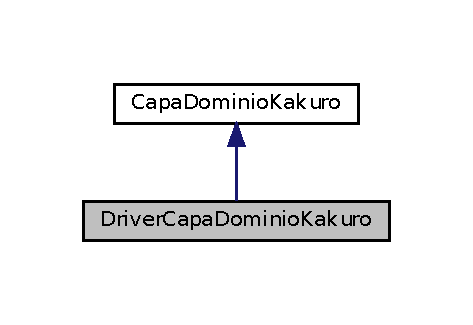
\includegraphics[width=227pt]{class_dominio_1_1controladores_1_1_drivers_1_1_driver_capa_dominio_kakuro__inherit__graph}
\end{center}
\end{figure}


Collaboration diagram for Driver\+Capa\+Dominio\+Kakuro\+:
\nopagebreak
\begin{figure}[H]
\begin{center}
\leavevmode
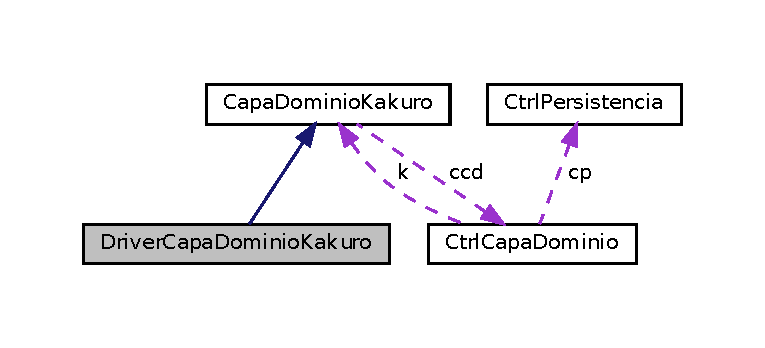
\includegraphics[width=350pt]{class_dominio_1_1controladores_1_1_drivers_1_1_driver_capa_dominio_kakuro__coll__graph}
\end{center}
\end{figure}
\subsection*{Static Public Member Functions}
\begin{DoxyCompactItemize}
\item 
\mbox{\label{class_dominio_1_1controladores_1_1_drivers_1_1_driver_capa_dominio_kakuro_a31b15a500be1892e96d81c271adffacb}} 
static void {\bfseries main} (String [$\,$] args)
\item 
static void \textbf{ test\+Generar\+Sumas} (\textbf{ Casilla}[$\,$][$\,$] k)
\begin{DoxyCompactList}\small\item\em Prueba el método generar\+Sumas. \end{DoxyCompactList}\item 
static void \textbf{ test\+Generar\+Casillas\+Blancas} (\textbf{ Casilla}[$\,$][$\,$] k)
\begin{DoxyCompactList}\small\item\em Prueba el método generarcasillas\+Blancas. \end{DoxyCompactList}\item 
static void \textbf{ test\+Generar\+Casillas\+Negras} (\textbf{ Casilla}[$\,$][$\,$] k, int negras)
\begin{DoxyCompactList}\small\item\em Prueba el método generarcasillas\+Negras. \end{DoxyCompactList}\item 
\mbox{\label{class_dominio_1_1controladores_1_1_drivers_1_1_driver_capa_dominio_kakuro_a095bf6bb9987aef63fdead5fc182be9d}} 
static void \textbf{ test\+Generar\+Kakuro} ()
\begin{DoxyCompactList}\small\item\em Prueba la funcion de generar\+Kakuro y sus métodos. \end{DoxyCompactList}\item 
\mbox{\label{class_dominio_1_1controladores_1_1_drivers_1_1_driver_capa_dominio_kakuro_ae027d444962131c8f646fbe49ff23632}} 
static void \textbf{ testtake\+Fila\+Columna} ()
\begin{DoxyCompactList}\small\item\em Prueba los metodos take\+Fila y take\+Columna. \end{DoxyCompactList}\item 
\mbox{\label{class_dominio_1_1controladores_1_1_drivers_1_1_driver_capa_dominio_kakuro_a9b25ae87e75143633e0c393c7fce6c1a}} 
static void \textbf{ test\+Check\+Run} ()
\begin{DoxyCompactList}\small\item\em Prueba el metodo check\+Run. \end{DoxyCompactList}\item 
static void \textbf{ test\+Solve} ()
\begin{DoxyCompactList}\small\item\em Prueba la función destinada a resolver un Kakuro mediante un juego de pruebas. \end{DoxyCompactList}\item 
static void \textbf{ test\+Generar} ()
\begin{DoxyCompactList}\small\item\em Prueba la función destinada a generar un Kakuro mediante una dificultad. \end{DoxyCompactList}\item 
static void \textbf{ test\+Generar\+Resolver} ()
\begin{DoxyCompactList}\small\item\em Prueba la función destinada a generar un Kakuro mediante una dificultad y resolverlo justo despues. \end{DoxyCompactList}\item 
static void \textbf{ test\+Validar\+Kakuro} ()
\begin{DoxyCompactList}\small\item\em Prueba la funcion validar\+Kakuro. \end{DoxyCompactList}\end{DoxyCompactItemize}
\subsection*{Additional Inherited Members}


\subsection{Detailed Description}
\begin{DoxyAuthor}{Author}
David Nogales 
\end{DoxyAuthor}


Definition at line 21 of file Driver\+Capa\+Dominio\+Kakuro.\+java.



\subsection{Member Function Documentation}
\mbox{\label{class_dominio_1_1controladores_1_1_drivers_1_1_driver_capa_dominio_kakuro_ac39d50ad7aea9aa181d385415da69acf}} 
\index{Dominio\+::controladores\+::\+Drivers\+::\+Driver\+Capa\+Dominio\+Kakuro@{Dominio\+::controladores\+::\+Drivers\+::\+Driver\+Capa\+Dominio\+Kakuro}!test\+Generar@{test\+Generar}}
\index{test\+Generar@{test\+Generar}!Dominio\+::controladores\+::\+Drivers\+::\+Driver\+Capa\+Dominio\+Kakuro@{Dominio\+::controladores\+::\+Drivers\+::\+Driver\+Capa\+Dominio\+Kakuro}}
\subsubsection{test\+Generar()}
{\footnotesize\ttfamily static void test\+Generar (\begin{DoxyParamCaption}{ }\end{DoxyParamCaption})\hspace{0.3cm}{\ttfamily [inline]}, {\ttfamily [static]}}



Prueba la función destinada a generar un Kakuro mediante una dificultad. 

\begin{DoxyPostcond}{Postcondition}
Kakuro tiene su solución guardada en un atributo privado y la muestra por pantalla. 
\end{DoxyPostcond}


Definition at line 277 of file Driver\+Capa\+Dominio\+Kakuro.\+java.

\mbox{\label{class_dominio_1_1controladores_1_1_drivers_1_1_driver_capa_dominio_kakuro_a57efc137e015cbceb01a752a828a409b}} 
\index{Dominio\+::controladores\+::\+Drivers\+::\+Driver\+Capa\+Dominio\+Kakuro@{Dominio\+::controladores\+::\+Drivers\+::\+Driver\+Capa\+Dominio\+Kakuro}!test\+Generar\+Casillas\+Blancas@{test\+Generar\+Casillas\+Blancas}}
\index{test\+Generar\+Casillas\+Blancas@{test\+Generar\+Casillas\+Blancas}!Dominio\+::controladores\+::\+Drivers\+::\+Driver\+Capa\+Dominio\+Kakuro@{Dominio\+::controladores\+::\+Drivers\+::\+Driver\+Capa\+Dominio\+Kakuro}}
\subsubsection{test\+Generar\+Casillas\+Blancas()}
{\footnotesize\ttfamily static void test\+Generar\+Casillas\+Blancas (\begin{DoxyParamCaption}\item[{\textbf{ Casilla}}]{k[$\,$][$\,$] }\end{DoxyParamCaption})\hspace{0.3cm}{\ttfamily [inline]}, {\ttfamily [static]}}



Prueba el método generarcasillas\+Blancas. 


\begin{DoxyParams}{Parameters}
{\em k} & = matriz de casillas con casillas negras \begin{DoxyVerb}@post k contiene el resultado de generarCasillasBlancas;\end{DoxyVerb}
 \\
\hline
\end{DoxyParams}


Definition at line 76 of file Driver\+Capa\+Dominio\+Kakuro.\+java.

\mbox{\label{class_dominio_1_1controladores_1_1_drivers_1_1_driver_capa_dominio_kakuro_a13519d0b4604f2d8e275727b51504de5}} 
\index{Dominio\+::controladores\+::\+Drivers\+::\+Driver\+Capa\+Dominio\+Kakuro@{Dominio\+::controladores\+::\+Drivers\+::\+Driver\+Capa\+Dominio\+Kakuro}!test\+Generar\+Casillas\+Negras@{test\+Generar\+Casillas\+Negras}}
\index{test\+Generar\+Casillas\+Negras@{test\+Generar\+Casillas\+Negras}!Dominio\+::controladores\+::\+Drivers\+::\+Driver\+Capa\+Dominio\+Kakuro@{Dominio\+::controladores\+::\+Drivers\+::\+Driver\+Capa\+Dominio\+Kakuro}}
\subsubsection{test\+Generar\+Casillas\+Negras()}
{\footnotesize\ttfamily static void test\+Generar\+Casillas\+Negras (\begin{DoxyParamCaption}\item[{\textbf{ Casilla}}]{k[$\,$][$\,$],  }\item[{int}]{negras }\end{DoxyParamCaption})\hspace{0.3cm}{\ttfamily [inline]}, {\ttfamily [static]}}



Prueba el método generarcasillas\+Negras. 


\begin{DoxyParams}{Parameters}
{\em k} & = matriz de casillas vacía \\
\hline
{\em negras} & = número de casillas negras a generar \\
\hline
\end{DoxyParams}
\begin{DoxyPostcond}{Postcondition}
k contiene el resultado de generar\+Casillas\+Negras; 
\end{DoxyPostcond}


Definition at line 99 of file Driver\+Capa\+Dominio\+Kakuro.\+java.

\mbox{\label{class_dominio_1_1controladores_1_1_drivers_1_1_driver_capa_dominio_kakuro_a326ff1b40333ae3c6cdddf26bbb629e6}} 
\index{Dominio\+::controladores\+::\+Drivers\+::\+Driver\+Capa\+Dominio\+Kakuro@{Dominio\+::controladores\+::\+Drivers\+::\+Driver\+Capa\+Dominio\+Kakuro}!test\+Generar\+Resolver@{test\+Generar\+Resolver}}
\index{test\+Generar\+Resolver@{test\+Generar\+Resolver}!Dominio\+::controladores\+::\+Drivers\+::\+Driver\+Capa\+Dominio\+Kakuro@{Dominio\+::controladores\+::\+Drivers\+::\+Driver\+Capa\+Dominio\+Kakuro}}
\subsubsection{test\+Generar\+Resolver()}
{\footnotesize\ttfamily static void test\+Generar\+Resolver (\begin{DoxyParamCaption}{ }\end{DoxyParamCaption})\hspace{0.3cm}{\ttfamily [inline]}, {\ttfamily [static]}}



Prueba la función destinada a generar un Kakuro mediante una dificultad y resolverlo justo despues. 

\begin{DoxyPostcond}{Postcondition}
se muestra el resultado de generar y resolver por pantalla 
\end{DoxyPostcond}


Definition at line 306 of file Driver\+Capa\+Dominio\+Kakuro.\+java.

\mbox{\label{class_dominio_1_1controladores_1_1_drivers_1_1_driver_capa_dominio_kakuro_ad419fcca981c085e88799f107cea6c7c}} 
\index{Dominio\+::controladores\+::\+Drivers\+::\+Driver\+Capa\+Dominio\+Kakuro@{Dominio\+::controladores\+::\+Drivers\+::\+Driver\+Capa\+Dominio\+Kakuro}!test\+Generar\+Sumas@{test\+Generar\+Sumas}}
\index{test\+Generar\+Sumas@{test\+Generar\+Sumas}!Dominio\+::controladores\+::\+Drivers\+::\+Driver\+Capa\+Dominio\+Kakuro@{Dominio\+::controladores\+::\+Drivers\+::\+Driver\+Capa\+Dominio\+Kakuro}}
\subsubsection{test\+Generar\+Sumas()}
{\footnotesize\ttfamily static void test\+Generar\+Sumas (\begin{DoxyParamCaption}\item[{\textbf{ Casilla}}]{k[$\,$][$\,$] }\end{DoxyParamCaption})\hspace{0.3cm}{\ttfamily [inline]}, {\ttfamily [static]}}



Prueba el método generar\+Sumas. 


\begin{DoxyParams}{Parameters}
{\em k} & = matriz de casillas con casillas negras y blancas \begin{DoxyVerb}@post k contiene el resultado de generarSumas;\end{DoxyVerb}
 \\
\hline
\end{DoxyParams}


Definition at line 56 of file Driver\+Capa\+Dominio\+Kakuro.\+java.

\mbox{\label{class_dominio_1_1controladores_1_1_drivers_1_1_driver_capa_dominio_kakuro_a02ea25d515e18d85c09a31aaf6177a86}} 
\index{Dominio\+::controladores\+::\+Drivers\+::\+Driver\+Capa\+Dominio\+Kakuro@{Dominio\+::controladores\+::\+Drivers\+::\+Driver\+Capa\+Dominio\+Kakuro}!test\+Solve@{test\+Solve}}
\index{test\+Solve@{test\+Solve}!Dominio\+::controladores\+::\+Drivers\+::\+Driver\+Capa\+Dominio\+Kakuro@{Dominio\+::controladores\+::\+Drivers\+::\+Driver\+Capa\+Dominio\+Kakuro}}
\subsubsection{test\+Solve()}
{\footnotesize\ttfamily static void test\+Solve (\begin{DoxyParamCaption}{ }\end{DoxyParamCaption})\hspace{0.3cm}{\ttfamily [inline]}, {\ttfamily [static]}}



Prueba la función destinada a resolver un Kakuro mediante un juego de pruebas. 

\begin{DoxyPostcond}{Postcondition}
Kakuro tiene su solución guardada en un atributo privado y la muestra por pantalla. 
\end{DoxyPostcond}


Definition at line 240 of file Driver\+Capa\+Dominio\+Kakuro.\+java.

\mbox{\label{class_dominio_1_1controladores_1_1_drivers_1_1_driver_capa_dominio_kakuro_a883b13b5bef1544bea740e04121d3f67}} 
\index{Dominio\+::controladores\+::\+Drivers\+::\+Driver\+Capa\+Dominio\+Kakuro@{Dominio\+::controladores\+::\+Drivers\+::\+Driver\+Capa\+Dominio\+Kakuro}!test\+Validar\+Kakuro@{test\+Validar\+Kakuro}}
\index{test\+Validar\+Kakuro@{test\+Validar\+Kakuro}!Dominio\+::controladores\+::\+Drivers\+::\+Driver\+Capa\+Dominio\+Kakuro@{Dominio\+::controladores\+::\+Drivers\+::\+Driver\+Capa\+Dominio\+Kakuro}}
\subsubsection{test\+Validar\+Kakuro()}
{\footnotesize\ttfamily static void test\+Validar\+Kakuro (\begin{DoxyParamCaption}{ }\end{DoxyParamCaption})\hspace{0.3cm}{\ttfamily [inline]}, {\ttfamily [static]}}



Prueba la funcion validar\+Kakuro. 

\begin{DoxyPostcond}{Postcondition}
se muestra el resultado de validar por pantalla en caso de que funcione correctamente 
\end{DoxyPostcond}


Definition at line 334 of file Driver\+Capa\+Dominio\+Kakuro.\+java.



The documentation for this class was generated from the following file\+:\begin{DoxyCompactItemize}
\item 
src/\+Dominio/controladores/\+Drivers/Driver\+Capa\+Dominio\+Kakuro.\+java\end{DoxyCompactItemize}

\section{Driver\+Partida Class Reference}
\label{class_dominio_1_1controladores_1_1_drivers_1_1_driver_partida}\index{Driver\+Partida@{Driver\+Partida}}


Inheritance diagram for Driver\+Partida\+:
\nopagebreak
\begin{figure}[H]
\begin{center}
\leavevmode
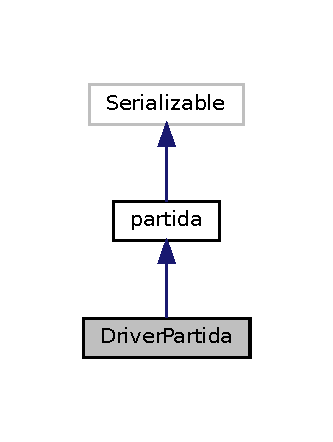
\includegraphics[width=160pt]{class_dominio_1_1controladores_1_1_drivers_1_1_driver_partida__inherit__graph}
\end{center}
\end{figure}


Collaboration diagram for Driver\+Partida\+:
\nopagebreak
\begin{figure}[H]
\begin{center}
\leavevmode
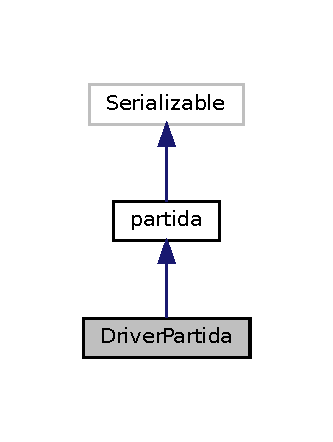
\includegraphics[width=160pt]{class_dominio_1_1controladores_1_1_drivers_1_1_driver_partida__coll__graph}
\end{center}
\end{figure}
\subsection*{Static Public Member Functions}
\begin{DoxyCompactItemize}
\item 
\mbox{\label{class_dominio_1_1controladores_1_1_drivers_1_1_driver_partida_a31b15a500be1892e96d81c271adffacb}} 
static void {\bfseries main} (String [$\,$] args)
\end{DoxyCompactItemize}
\subsection*{Additional Inherited Members}


\subsection{Detailed Description}
\begin{DoxyAuthor}{Author}
perem 
\end{DoxyAuthor}


Definition at line 21 of file Driver\+Partida.\+java.



The documentation for this class was generated from the following file\+:\begin{DoxyCompactItemize}
\item 
src/\+Dominio/controladores/\+Drivers/Driver\+Partida.\+java\end{DoxyCompactItemize}

\section{Guardar\+Partida\+Dialog Class Reference}
\label{class_presentacion_1_1_guardar_partida_dialog}\index{Guardar\+Partida\+Dialog@{Guardar\+Partida\+Dialog}}


Clase que implementa el diálogo para poner nombre a una partida guardada.  




Inheritance diagram for Guardar\+Partida\+Dialog\+:
\nopagebreak
\begin{figure}[H]
\begin{center}
\leavevmode
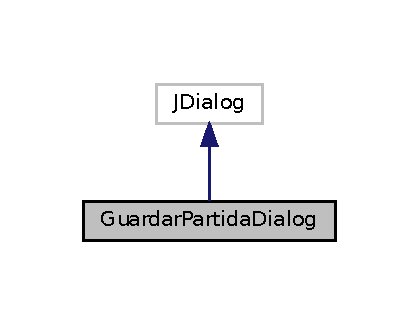
\includegraphics[width=201pt]{class_presentacion_1_1_guardar_partida_dialog__inherit__graph}
\end{center}
\end{figure}


Collaboration diagram for Guardar\+Partida\+Dialog\+:
\nopagebreak
\begin{figure}[H]
\begin{center}
\leavevmode
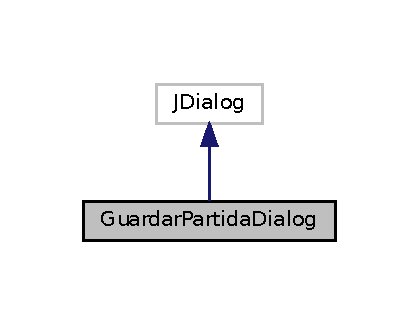
\includegraphics[width=201pt]{class_presentacion_1_1_guardar_partida_dialog__coll__graph}
\end{center}
\end{figure}
\subsection*{Public Member Functions}
\begin{DoxyCompactItemize}
\item 
\mbox{\label{class_presentacion_1_1_guardar_partida_dialog_af2a175ac9dd7d282e20d3390492e0f7d}} 
{\bfseries Guardar\+Partida\+Dialog} (java.\+awt.\+Frame parent, boolean modal)
\item 
\mbox{\label{class_presentacion_1_1_guardar_partida_dialog_a00665a0e7ffb74a58a1beca66d87d8ed}} 
{\bfseries Guardar\+Partida\+Dialog} (\textbf{ Vista\+Kakuro} vk)
\item 
\mbox{\label{class_presentacion_1_1_guardar_partida_dialog_a58b6a37bf49b31de62d02749a9a37d87}} 
void {\bfseries not\+Save} ()
\end{DoxyCompactItemize}
\subsection*{Static Public Member Functions}
\begin{DoxyCompactItemize}
\item 
static void \textbf{ main} (String args[$\,$])
\end{DoxyCompactItemize}


\subsection{Detailed Description}
Clase que implementa el diálogo para poner nombre a una partida guardada. 

Definition at line 21 of file Guardar\+Partida\+Dialog.\+java.



\subsection{Member Function Documentation}
\mbox{\label{class_presentacion_1_1_guardar_partida_dialog_a75988cf84fc6ee7a2ebff36e363021aa}} 
\index{Presentacion\+::\+Guardar\+Partida\+Dialog@{Presentacion\+::\+Guardar\+Partida\+Dialog}!main@{main}}
\index{main@{main}!Presentacion\+::\+Guardar\+Partida\+Dialog@{Presentacion\+::\+Guardar\+Partida\+Dialog}}
\subsubsection{main()}
{\footnotesize\ttfamily static void main (\begin{DoxyParamCaption}\item[{String}]{args[$\,$] }\end{DoxyParamCaption})\hspace{0.3cm}{\ttfamily [inline]}, {\ttfamily [static]}}


\begin{DoxyParams}{Parameters}
{\em args} & the command line arguments \\
\hline
\end{DoxyParams}


Definition at line 131 of file Guardar\+Partida\+Dialog.\+java.



The documentation for this class was generated from the following file\+:\begin{DoxyCompactItemize}
\item 
src/\+Presentacion/Guardar\+Partida\+Dialog.\+java\end{DoxyCompactItemize}

\section{Kakuro Class Reference}
\label{class_dominio_1_1clases_1_1_kakuro}\index{Kakuro@{Kakuro}}


Clase que representa un kakuro. Contiene su tablero tanto información sobre el mismo.  




Inheritance diagram for Kakuro\+:
\nopagebreak
\begin{figure}[H]
\begin{center}
\leavevmode
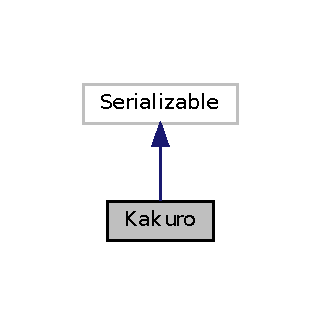
\includegraphics[width=154pt]{class_dominio_1_1clases_1_1_kakuro__inherit__graph}
\end{center}
\end{figure}


Collaboration diagram for Kakuro\+:
\nopagebreak
\begin{figure}[H]
\begin{center}
\leavevmode
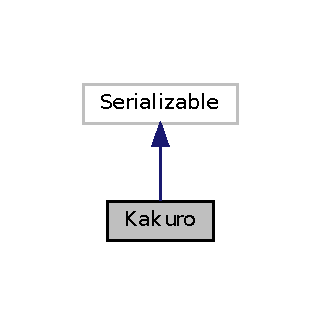
\includegraphics[width=154pt]{class_dominio_1_1clases_1_1_kakuro__coll__graph}
\end{center}
\end{figure}
\subsection*{Public Member Functions}
\begin{DoxyCompactItemize}
\item 
\textbf{ Kakuro} ()
\begin{DoxyCompactList}\small\item\em Constructora de kakuro. \end{DoxyCompactList}\item 
\textbf{ Kakuro} (int c\+\_\+blancas, int c\+\_\+negras, \textbf{ Casilla} [$\,$][$\,$] k)
\begin{DoxyCompactList}\small\item\em Constructora de \doxyref{Kakuro}{p.}{class_dominio_1_1clases_1_1_kakuro}. \end{DoxyCompactList}\item 
void \textbf{ set\+Blancas} (int b)
\begin{DoxyCompactList}\small\item\em Modifica el valor de celdas\+\_\+blancas. \end{DoxyCompactList}\item 
int \textbf{ get\+Filas} ()
\begin{DoxyCompactList}\small\item\em Consultora del las filas del kakuro. \end{DoxyCompactList}\item 
int \textbf{ get\+Columnas} ()
\begin{DoxyCompactList}\small\item\em Consultora del las columnas del kakuro. \end{DoxyCompactList}\item 
\textbf{ Casilla} [$\,$][$\,$] \textbf{ get\+Tablero} ()
\begin{DoxyCompactList}\small\item\em Consultora del tablero del kakuro. \end{DoxyCompactList}\item 
int \textbf{ get\+I\+D\+\_\+\+Kakuro} ()
\begin{DoxyCompactList}\small\item\em Consultora del Identificador del kakuro. \end{DoxyCompactList}\item 
void \textbf{ set\+I\+D\+\_\+\+Kakuro} (int id)
\begin{DoxyCompactList}\small\item\em Modificadora del ID de \doxyref{Kakuro}{p.}{class_dominio_1_1clases_1_1_kakuro}. \end{DoxyCompactList}\item 
int \textbf{ getceldas\+\_\+blancas} ()
\begin{DoxyCompactList}\small\item\em Consultora de las soluciones del kakuro. \end{DoxyCompactList}\item 
int \textbf{ getceldas\+\_\+negras} ()
\begin{DoxyCompactList}\small\item\em Consultora del numero de celdas negras del kakuro. \end{DoxyCompactList}\item 
\mbox{\label{class_dominio_1_1clases_1_1_kakuro_a9b80dd6d8e29a4aa4b47a07388baff19}} 
void {\bfseries print\+Grid} ()
\item 
\mbox{\label{class_dominio_1_1clases_1_1_kakuro_a0315a918ba5b494fb4f010e09d763e60}} 
void {\bfseries Stringto\+Grid} (String k)
\item 
\mbox{\label{class_dominio_1_1clases_1_1_kakuro_a6b9732f93998f32d752843518a41239f}} 
void {\bfseries set\+Dif} (double dif)
\item 
\mbox{\label{class_dominio_1_1clases_1_1_kakuro_af497e1c6b31715638bfc30c67b1756b4}} 
double {\bfseries get\+Dif} ()
\end{DoxyCompactItemize}


\subsection{Detailed Description}
Clase que representa un kakuro. Contiene su tablero tanto información sobre el mismo. 

Definition at line 27 of file Kakuro.\+java.



\subsection{Constructor \& Destructor Documentation}
\mbox{\label{class_dominio_1_1clases_1_1_kakuro_adec990e3614f516b12661ff0ed467f92}} 
\index{Dominio\+::clases\+::\+Kakuro@{Dominio\+::clases\+::\+Kakuro}!Kakuro@{Kakuro}}
\index{Kakuro@{Kakuro}!Dominio\+::clases\+::\+Kakuro@{Dominio\+::clases\+::\+Kakuro}}
\subsubsection{Kakuro()\hspace{0.1cm}{\footnotesize\ttfamily [1/2]}}
{\footnotesize\ttfamily \textbf{ Kakuro} (\begin{DoxyParamCaption}{ }\end{DoxyParamCaption})\hspace{0.3cm}{\ttfamily [inline]}}



Constructora de kakuro. 

\begin{DoxyPostcond}{Postcondition}
crea un kakuro null 
\end{DoxyPostcond}


Definition at line 54 of file Kakuro.\+java.

\mbox{\label{class_dominio_1_1clases_1_1_kakuro_af727cbfb747a04b03eda399125e5d23f}} 
\index{Dominio\+::clases\+::\+Kakuro@{Dominio\+::clases\+::\+Kakuro}!Kakuro@{Kakuro}}
\index{Kakuro@{Kakuro}!Dominio\+::clases\+::\+Kakuro@{Dominio\+::clases\+::\+Kakuro}}
\subsubsection{Kakuro()\hspace{0.1cm}{\footnotesize\ttfamily [2/2]}}
{\footnotesize\ttfamily \textbf{ Kakuro} (\begin{DoxyParamCaption}\item[{int}]{c\+\_\+blancas,  }\item[{int}]{c\+\_\+negras,  }\item[{\textbf{ Casilla}}]{k[$\,$][$\,$] }\end{DoxyParamCaption})\hspace{0.3cm}{\ttfamily [inline]}}



Constructora de \doxyref{Kakuro}{p.}{class_dominio_1_1clases_1_1_kakuro}. 


\begin{DoxyParams}{Parameters}
{\em c\+\_\+blancas} & = numero de casillas blancas del kakuro \\
\hline
{\em c\+\_\+megras} & = numero de casillas negras del kakuro \\
\hline
{\em k} & = matriz de casillas que represnta el tablero\\
\hline
\end{DoxyParams}
\begin{DoxyPostcond}{Postcondition}
Se creará un kakuro con esos parámetros 
\end{DoxyPostcond}


Definition at line 65 of file Kakuro.\+java.



\subsection{Member Function Documentation}
\mbox{\label{class_dominio_1_1clases_1_1_kakuro_a5b5d13352a6553be938e417f987c392f}} 
\index{Dominio\+::clases\+::\+Kakuro@{Dominio\+::clases\+::\+Kakuro}!getceldas\+\_\+blancas@{getceldas\+\_\+blancas}}
\index{getceldas\+\_\+blancas@{getceldas\+\_\+blancas}!Dominio\+::clases\+::\+Kakuro@{Dominio\+::clases\+::\+Kakuro}}
\subsubsection{getceldas\+\_\+blancas()}
{\footnotesize\ttfamily int getceldas\+\_\+blancas (\begin{DoxyParamCaption}{ }\end{DoxyParamCaption})\hspace{0.3cm}{\ttfamily [inline]}}



Consultora de las soluciones del kakuro. 

\begin{DoxyPostcond}{Postcondition}
Devuelve un vector con las soluciones del kakuro Consultora del numero de celdas blancas del kakuro

Devuelve el numero de celdas blancas del kakuro 
\end{DoxyPostcond}


Definition at line 138 of file Kakuro.\+java.

\mbox{\label{class_dominio_1_1clases_1_1_kakuro_acf98d73784f1c017662808c6cc13f368}} 
\index{Dominio\+::clases\+::\+Kakuro@{Dominio\+::clases\+::\+Kakuro}!getceldas\+\_\+negras@{getceldas\+\_\+negras}}
\index{getceldas\+\_\+negras@{getceldas\+\_\+negras}!Dominio\+::clases\+::\+Kakuro@{Dominio\+::clases\+::\+Kakuro}}
\subsubsection{getceldas\+\_\+negras()}
{\footnotesize\ttfamily int getceldas\+\_\+negras (\begin{DoxyParamCaption}{ }\end{DoxyParamCaption})\hspace{0.3cm}{\ttfamily [inline]}}



Consultora del numero de celdas negras del kakuro. 

\begin{DoxyPostcond}{Postcondition}
Devuelve el numero de celdas negras del kakuro 
\end{DoxyPostcond}


Definition at line 146 of file Kakuro.\+java.

\mbox{\label{class_dominio_1_1clases_1_1_kakuro_a519328ddfad2352c4ddcd609ed53b8a6}} 
\index{Dominio\+::clases\+::\+Kakuro@{Dominio\+::clases\+::\+Kakuro}!get\+Columnas@{get\+Columnas}}
\index{get\+Columnas@{get\+Columnas}!Dominio\+::clases\+::\+Kakuro@{Dominio\+::clases\+::\+Kakuro}}
\subsubsection{get\+Columnas()}
{\footnotesize\ttfamily int get\+Columnas (\begin{DoxyParamCaption}{ }\end{DoxyParamCaption})\hspace{0.3cm}{\ttfamily [inline]}}



Consultora del las columnas del kakuro. 

\begin{DoxyPostcond}{Postcondition}
Devuelve el numero de columnas del kakuro 
\end{DoxyPostcond}


Definition at line 98 of file Kakuro.\+java.

\mbox{\label{class_dominio_1_1clases_1_1_kakuro_a9797970b65d6e75bb257187536d50715}} 
\index{Dominio\+::clases\+::\+Kakuro@{Dominio\+::clases\+::\+Kakuro}!get\+Filas@{get\+Filas}}
\index{get\+Filas@{get\+Filas}!Dominio\+::clases\+::\+Kakuro@{Dominio\+::clases\+::\+Kakuro}}
\subsubsection{get\+Filas()}
{\footnotesize\ttfamily int get\+Filas (\begin{DoxyParamCaption}{ }\end{DoxyParamCaption})\hspace{0.3cm}{\ttfamily [inline]}}



Consultora del las filas del kakuro. 

\begin{DoxyPostcond}{Postcondition}
Devuelve el numero de filas del kakuro 
\end{DoxyPostcond}


Definition at line 89 of file Kakuro.\+java.

\mbox{\label{class_dominio_1_1clases_1_1_kakuro_a06c7f4b0dfa1850e3995751c257f5c79}} 
\index{Dominio\+::clases\+::\+Kakuro@{Dominio\+::clases\+::\+Kakuro}!get\+I\+D\+\_\+\+Kakuro@{get\+I\+D\+\_\+\+Kakuro}}
\index{get\+I\+D\+\_\+\+Kakuro@{get\+I\+D\+\_\+\+Kakuro}!Dominio\+::clases\+::\+Kakuro@{Dominio\+::clases\+::\+Kakuro}}
\subsubsection{get\+I\+D\+\_\+\+Kakuro()}
{\footnotesize\ttfamily int get\+I\+D\+\_\+\+Kakuro (\begin{DoxyParamCaption}{ }\end{DoxyParamCaption})\hspace{0.3cm}{\ttfamily [inline]}}



Consultora del Identificador del kakuro. 

\begin{DoxyPostcond}{Postcondition}
Devuelve el ID del kakuro 
\end{DoxyPostcond}


Definition at line 116 of file Kakuro.\+java.

\mbox{\label{class_dominio_1_1clases_1_1_kakuro_a0a6a4a20caa9f4f291f89d70e802f3d1}} 
\index{Dominio\+::clases\+::\+Kakuro@{Dominio\+::clases\+::\+Kakuro}!get\+Tablero@{get\+Tablero}}
\index{get\+Tablero@{get\+Tablero}!Dominio\+::clases\+::\+Kakuro@{Dominio\+::clases\+::\+Kakuro}}
\subsubsection{get\+Tablero()}
{\footnotesize\ttfamily \textbf{ Casilla} [$\,$][$\,$] get\+Tablero (\begin{DoxyParamCaption}{ }\end{DoxyParamCaption})\hspace{0.3cm}{\ttfamily [inline]}}



Consultora del tablero del kakuro. 

\begin{DoxyPostcond}{Postcondition}
Devuelve una matriz de casillas que representa el kakuro 
\end{DoxyPostcond}


Definition at line 107 of file Kakuro.\+java.

\mbox{\label{class_dominio_1_1clases_1_1_kakuro_ab34b730a714826c508a11d9ac2d17bd7}} 
\index{Dominio\+::clases\+::\+Kakuro@{Dominio\+::clases\+::\+Kakuro}!set\+Blancas@{set\+Blancas}}
\index{set\+Blancas@{set\+Blancas}!Dominio\+::clases\+::\+Kakuro@{Dominio\+::clases\+::\+Kakuro}}
\subsubsection{set\+Blancas()}
{\footnotesize\ttfamily void set\+Blancas (\begin{DoxyParamCaption}\item[{int}]{b }\end{DoxyParamCaption})\hspace{0.3cm}{\ttfamily [inline]}}



Modifica el valor de celdas\+\_\+blancas. 


\begin{DoxyParams}{Parameters}
{\em b} & = nuevo valor de celdas\+\_\+blancas \\
\hline
\end{DoxyParams}
\begin{DoxyPostcond}{Postcondition}
celdas\+\_\+blancas = b 
\end{DoxyPostcond}


Definition at line 80 of file Kakuro.\+java.

\mbox{\label{class_dominio_1_1clases_1_1_kakuro_aa9b58618f7e49faf686d237993d30db3}} 
\index{Dominio\+::clases\+::\+Kakuro@{Dominio\+::clases\+::\+Kakuro}!set\+I\+D\+\_\+\+Kakuro@{set\+I\+D\+\_\+\+Kakuro}}
\index{set\+I\+D\+\_\+\+Kakuro@{set\+I\+D\+\_\+\+Kakuro}!Dominio\+::clases\+::\+Kakuro@{Dominio\+::clases\+::\+Kakuro}}
\subsubsection{set\+I\+D\+\_\+\+Kakuro()}
{\footnotesize\ttfamily void set\+I\+D\+\_\+\+Kakuro (\begin{DoxyParamCaption}\item[{int}]{id }\end{DoxyParamCaption})\hspace{0.3cm}{\ttfamily [inline]}}



Modificadora del ID de \doxyref{Kakuro}{p.}{class_dominio_1_1clases_1_1_kakuro}. 


\begin{DoxyParams}{Parameters}
{\em id} & = nuevo identificador \\
\hline
\end{DoxyParams}
\begin{DoxyPostcond}{Postcondition}
ID modificado 
\end{DoxyPostcond}


Definition at line 123 of file Kakuro.\+java.



The documentation for this class was generated from the following file\+:\begin{DoxyCompactItemize}
\item 
src/\+Dominio/clases/\textbf{ Kakuro.\+java}\end{DoxyCompactItemize}

\section{Kakuro\+\_\+\+Game Class Reference}
\label{class_dominio_1_1clases_1_1_kakuro___game}\index{Kakuro\+\_\+\+Game@{Kakuro\+\_\+\+Game}}
\subsection*{Static Public Member Functions}
\begin{DoxyCompactItemize}
\item 
\mbox{\label{class_dominio_1_1clases_1_1_kakuro___game_a8b260eecbaabcef8473fd87ada040682}} 
static void {\bfseries main} (String[$\,$] args)
\end{DoxyCompactItemize}


\subsection{Detailed Description}


Definition at line 27 of file Kakuro\+\_\+\+Game.\+java.



The documentation for this class was generated from the following file\+:\begin{DoxyCompactItemize}
\item 
src/\+Dominio/clases/\textbf{ Kakuro\+\_\+\+Game.\+java}\end{DoxyCompactItemize}

\section{partida Class Reference}
\label{class_dominio_1_1clases_1_1partida}\index{partida@{partida}}


Clase que representa una partida. Cada partida consiste en el id del usuario que la guarda, un identificador de partida, el tiempo transcurrido y el \doxyref{Kakuro}{p.}{class_dominio_1_1clases_1_1_kakuro} en juego.  




Inheritance diagram for partida\+:
\nopagebreak
\begin{figure}[H]
\begin{center}
\leavevmode
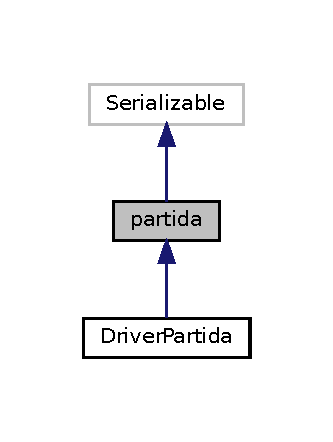
\includegraphics[width=160pt]{class_dominio_1_1clases_1_1partida__inherit__graph}
\end{center}
\end{figure}


Collaboration diagram for partida\+:
\nopagebreak
\begin{figure}[H]
\begin{center}
\leavevmode
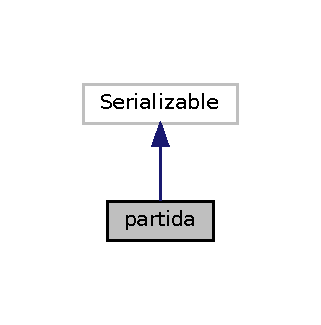
\includegraphics[width=154pt]{class_dominio_1_1clases_1_1partida__coll__graph}
\end{center}
\end{figure}
\subsection*{Public Member Functions}
\begin{DoxyCompactItemize}
\item 
\mbox{\label{class_dominio_1_1clases_1_1partida_a64938f1527c5975fb291e95242cb7364}} 
{\bfseries partida} (\textbf{ Kakuro} x, String Usuario)
\item 
\mbox{\label{class_dominio_1_1clases_1_1partida_a0e7e5c5893a966e3fd8f5f30550c6fe9}} 
{\bfseries partida} (String Usuario, String ID, \textbf{ Kakuro} x, int time)
\item 
\mbox{\label{class_dominio_1_1clases_1_1partida_ae43c95d31e5ff373cec8a3753bf6a3bd}} 
\textbf{ Kakuro} {\bfseries get\+Kakuro} ()
\item 
\mbox{\label{class_dominio_1_1clases_1_1partida_a6d4c17940d960c32be6a2d89746c29fa}} 
void {\bfseries set\+Kakuro} (\textbf{ Kakuro} kak)
\item 
\mbox{\label{class_dominio_1_1clases_1_1partida_a34e60b6081b4c555dc9f5b872cbe044e}} 
String {\bfseries get\+ID} ()
\item 
\mbox{\label{class_dominio_1_1clases_1_1partida_af7ae4772721a06996d1b110b929bd738}} 
String {\bfseries get\+I\+D\+Partida} ()
\item 
\mbox{\label{class_dominio_1_1clases_1_1partida_a8b75a4197e47fd5e553fae6eb8c48ff1}} 
void {\bfseries set\+Id\+Partida} (String nom)
\item 
\mbox{\label{class_dominio_1_1clases_1_1partida_a45d742d743ec93b9bc2d225b74264111}} 
void {\bfseries set\+New\+Kakuro} (\textbf{ Kakuro} kak)
\item 
\mbox{\label{class_dominio_1_1clases_1_1partida_a6bc6f79347d1de076580e9e81e4ec246}} 
void {\bfseries set\+Time} (int time)
\item 
\mbox{\label{class_dominio_1_1clases_1_1partida_a140cd6eb747b445398503dedfd51785f}} 
int {\bfseries get\+Time} ()
\item 
\mbox{\label{class_dominio_1_1clases_1_1partida_aeb0591352ec18ebccca332dedb03bc59}} 
void {\bfseries escribir} ()
\end{DoxyCompactItemize}


\subsection{Detailed Description}
Clase que representa una partida. Cada partida consiste en el id del usuario que la guarda, un identificador de partida, el tiempo transcurrido y el \doxyref{Kakuro}{p.}{class_dominio_1_1clases_1_1_kakuro} en juego. 

Definition at line 33 of file partida.\+java.



The documentation for this class was generated from the following file\+:\begin{DoxyCompactItemize}
\item 
src/\+Dominio/clases/\textbf{ partida.\+java}\end{DoxyCompactItemize}

\section{Vista\+Cargar\+Partida Class Reference}
\label{class_presentacion_1_1_vista_cargar_partida}\index{Vista\+Cargar\+Partida@{Vista\+Cargar\+Partida}}


Clase que extiende J\+Panel que inicializa, gestiona y modifica el panel de la \doxyref{Vista\+Principal}{p.}{class_presentacion_1_1_vista_principal} para Cargar Partidas.  




Inheritance diagram for Vista\+Cargar\+Partida\+:
\nopagebreak
\begin{figure}[H]
\begin{center}
\leavevmode
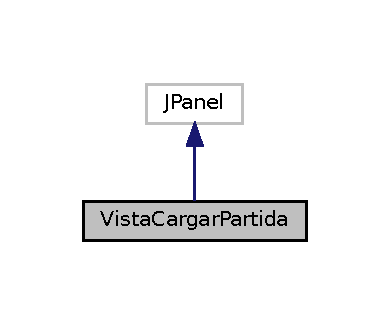
\includegraphics[width=187pt]{class_presentacion_1_1_vista_cargar_partida__inherit__graph}
\end{center}
\end{figure}


Collaboration diagram for Vista\+Cargar\+Partida\+:
\nopagebreak
\begin{figure}[H]
\begin{center}
\leavevmode
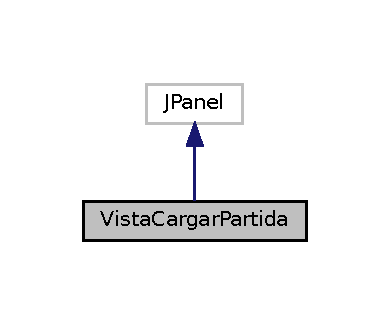
\includegraphics[width=187pt]{class_presentacion_1_1_vista_cargar_partida__coll__graph}
\end{center}
\end{figure}
\subsection*{Public Member Functions}
\begin{DoxyCompactItemize}
\item 
\textbf{ Vista\+Cargar\+Partida} ()
\item 
\mbox{\label{class_presentacion_1_1_vista_cargar_partida_ad67b4585e78cffb03ca746c7aa44785b}} 
{\bfseries Vista\+Cargar\+Partida} (\textbf{ Vista\+Principal} vista\+Principal)
\end{DoxyCompactItemize}


\subsection{Detailed Description}
Clase que extiende J\+Panel que inicializa, gestiona y modifica el panel de la \doxyref{Vista\+Principal}{p.}{class_presentacion_1_1_vista_principal} para Cargar Partidas. 

Definition at line 23 of file Vista\+Cargar\+Partida.\+java.



\subsection{Constructor \& Destructor Documentation}
\mbox{\label{class_presentacion_1_1_vista_cargar_partida_a420f4e3ccf2712708be5565b72c04ad1}} 
\index{Presentacion\+::\+Vista\+Cargar\+Partida@{Presentacion\+::\+Vista\+Cargar\+Partida}!Vista\+Cargar\+Partida@{Vista\+Cargar\+Partida}}
\index{Vista\+Cargar\+Partida@{Vista\+Cargar\+Partida}!Presentacion\+::\+Vista\+Cargar\+Partida@{Presentacion\+::\+Vista\+Cargar\+Partida}}
\subsubsection{Vista\+Cargar\+Partida()}
{\footnotesize\ttfamily \textbf{ Vista\+Cargar\+Partida} (\begin{DoxyParamCaption}{ }\end{DoxyParamCaption})\hspace{0.3cm}{\ttfamily [inline]}}

Creates new form \doxyref{Vista\+Cargar\+Partida}{p.}{class_presentacion_1_1_vista_cargar_partida} 

Definition at line 29 of file Vista\+Cargar\+Partida.\+java.



The documentation for this class was generated from the following file\+:\begin{DoxyCompactItemize}
\item 
src/\+Presentacion/\textbf{ Vista\+Cargar\+Partida.\+java}\end{DoxyCompactItemize}

\section{Vista\+Crear\+Kakuro Class Reference}
\label{class_presentacion_1_1_vista_crear_kakuro}\index{Vista\+Crear\+Kakuro@{Vista\+Crear\+Kakuro}}


Clase que extiende J\+Panel que inicializa, gestiona y modifica el panel de la \doxyref{Vista\+Principal}{p.}{class_presentacion_1_1_vista_principal} para Crear Kakuros.  




Inheritance diagram for Vista\+Crear\+Kakuro\+:
\nopagebreak
\begin{figure}[H]
\begin{center}
\leavevmode
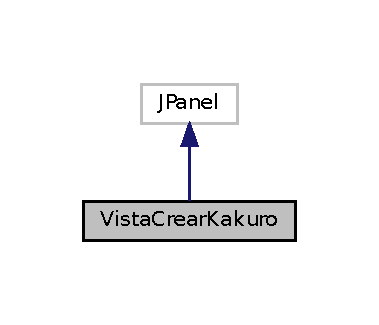
\includegraphics[width=182pt]{class_presentacion_1_1_vista_crear_kakuro__inherit__graph}
\end{center}
\end{figure}


Collaboration diagram for Vista\+Crear\+Kakuro\+:
\nopagebreak
\begin{figure}[H]
\begin{center}
\leavevmode
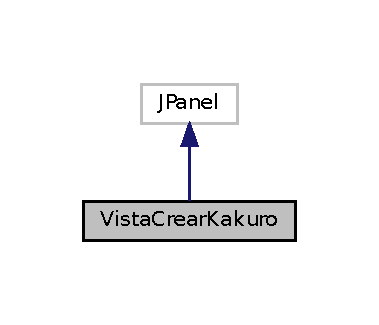
\includegraphics[width=182pt]{class_presentacion_1_1_vista_crear_kakuro__coll__graph}
\end{center}
\end{figure}
\subsection*{Public Member Functions}
\begin{DoxyCompactItemize}
\item 
\textbf{ Vista\+Crear\+Kakuro} ()
\item 
\mbox{\label{class_presentacion_1_1_vista_crear_kakuro_a5d8d8f80571d92a9b611a6d009a00c22}} 
void {\bfseries set\+Ultimo\+Kakuro\+Label} (int id)
\item 
\mbox{\label{class_presentacion_1_1_vista_crear_kakuro_ac5c96422f5891e6fbf8d7c286f61b82e}} 
void {\bfseries set\+Dificultad\+Label} (String dif)
\end{DoxyCompactItemize}


\subsection{Detailed Description}
Clase que extiende J\+Panel que inicializa, gestiona y modifica el panel de la \doxyref{Vista\+Principal}{p.}{class_presentacion_1_1_vista_principal} para Crear Kakuros. 

Definition at line 26 of file Vista\+Crear\+Kakuro.\+java.



\subsection{Constructor \& Destructor Documentation}
\mbox{\label{class_presentacion_1_1_vista_crear_kakuro_aa61712b3641d5cc127e82409a485b45a}} 
\index{Presentacion\+::\+Vista\+Crear\+Kakuro@{Presentacion\+::\+Vista\+Crear\+Kakuro}!Vista\+Crear\+Kakuro@{Vista\+Crear\+Kakuro}}
\index{Vista\+Crear\+Kakuro@{Vista\+Crear\+Kakuro}!Presentacion\+::\+Vista\+Crear\+Kakuro@{Presentacion\+::\+Vista\+Crear\+Kakuro}}
\subsubsection{Vista\+Crear\+Kakuro()}
{\footnotesize\ttfamily \textbf{ Vista\+Crear\+Kakuro} (\begin{DoxyParamCaption}{ }\end{DoxyParamCaption})\hspace{0.3cm}{\ttfamily [inline]}}

Creates new form \doxyref{Vista\+Crear\+Kakuro}{p.}{class_presentacion_1_1_vista_crear_kakuro} 

Definition at line 32 of file Vista\+Crear\+Kakuro.\+java.



The documentation for this class was generated from the following file\+:\begin{DoxyCompactItemize}
\item 
src/\+Presentacion/\textbf{ Vista\+Crear\+Kakuro.\+java}\end{DoxyCompactItemize}

\section{Vista\+Gestion\+Perfil Class Reference}
\label{class_presentacion_1_1_vista_gestion_perfil}\index{Vista\+Gestion\+Perfil@{Vista\+Gestion\+Perfil}}


Clase que inicializa, gestiona y modifica la Vista que controla el inicio de sesión y registro en el programa.  


\subsection*{Public Member Functions}
\begin{DoxyCompactItemize}
\item 
\mbox{\label{class_presentacion_1_1_vista_gestion_perfil_a767cae33dca3e1ae6ef022e0284aa891}} 
void {\bfseries change\+To\+Sign\+Up} ()
\item 
\mbox{\label{class_presentacion_1_1_vista_gestion_perfil_a5792059a35dca9e4c029fdb31a117819}} 
void {\bfseries change\+To\+Log\+In} ()
\item 
\mbox{\label{class_presentacion_1_1_vista_gestion_perfil_ad57530714d88f506d201d718395cf577}} 
boolean {\bfseries Log\+In} (String User, char[$\,$] Pass)
\item 
\mbox{\label{class_presentacion_1_1_vista_gestion_perfil_a8a4e10e8094cac30e3c5536b3a2364ae}} 
boolean {\bfseries Sign\+Up} (String User, char[$\,$] Pass)
\item 
\mbox{\label{class_presentacion_1_1_vista_gestion_perfil_a193026f0fe44beaa3a4b311179200d24}} 
void {\bfseries set\+Usuario} (String User)
\end{DoxyCompactItemize}


\subsection{Detailed Description}
Clase que inicializa, gestiona y modifica la Vista que controla el inicio de sesión y registro en el programa. 

Definition at line 29 of file Vista\+Gestion\+Perfil.\+java.



The documentation for this class was generated from the following file\+:\begin{DoxyCompactItemize}
\item 
src/\+Presentacion/\textbf{ Vista\+Gestion\+Perfil.\+java}\end{DoxyCompactItemize}

\section{Vista\+Kakuro Class Reference}
\label{class_presentacion_1_1_vista_kakuro}\index{Vista\+Kakuro@{Vista\+Kakuro}}


Clase que extiende J\+Panel que inicializa, gestiona y modifica el panel de la \doxyref{Vista\+Principal}{p.}{class_presentacion_1_1_vista_principal} para jugar un Kakuro.  




Inheritance diagram for Vista\+Kakuro\+:
\nopagebreak
\begin{figure}[H]
\begin{center}
\leavevmode
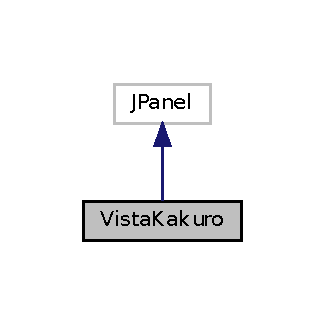
\includegraphics[width=156pt]{class_presentacion_1_1_vista_kakuro__inherit__graph}
\end{center}
\end{figure}


Collaboration diagram for Vista\+Kakuro\+:
\nopagebreak
\begin{figure}[H]
\begin{center}
\leavevmode
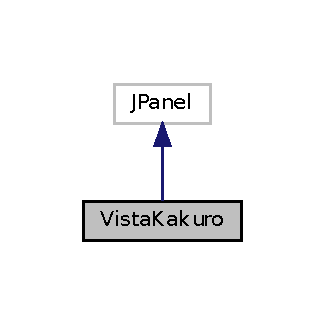
\includegraphics[width=156pt]{class_presentacion_1_1_vista_kakuro__coll__graph}
\end{center}
\end{figure}
\subsection*{Public Member Functions}
\begin{DoxyCompactItemize}
\item 
\textbf{ Vista\+Kakuro} ()
\item 
\mbox{\label{class_presentacion_1_1_vista_kakuro_a19354481f6fdaa342fa0b761e18a8ec2}} 
void {\bfseries display\+Kakuro} (int dimensiones, boolean edition\+Mode, boolean play\+After\+Edition, String [$\,$][$\,$] tablero)
\item 
\mbox{\label{class_presentacion_1_1_vista_kakuro_a3642ae4961bfedc57749e914ead03852}} 
void {\bfseries set\+Time\+In\+Label} ()
\item 
\mbox{\label{class_presentacion_1_1_vista_kakuro_aedf63d49e472a3ac3ca2d4085e7d2a32}} 
void {\bfseries set\+Ini\+Time} (int ini)
\item 
\mbox{\label{class_presentacion_1_1_vista_kakuro_a848fb8f044d4f5a682ea18de8ae12dc2}} 
void {\bfseries set\+Nombre\+Partida} (String nombre)
\end{DoxyCompactItemize}


\subsection{Detailed Description}
Clase que extiende J\+Panel que inicializa, gestiona y modifica el panel de la \doxyref{Vista\+Principal}{p.}{class_presentacion_1_1_vista_principal} para jugar un Kakuro. 

Definition at line 36 of file Vista\+Kakuro.\+java.



\subsection{Constructor \& Destructor Documentation}
\mbox{\label{class_presentacion_1_1_vista_kakuro_a6a5fddfdbcd08c83e77b53c33ca69414}} 
\index{Presentacion\+::\+Vista\+Kakuro@{Presentacion\+::\+Vista\+Kakuro}!Vista\+Kakuro@{Vista\+Kakuro}}
\index{Vista\+Kakuro@{Vista\+Kakuro}!Presentacion\+::\+Vista\+Kakuro@{Presentacion\+::\+Vista\+Kakuro}}
\subsubsection{Vista\+Kakuro()}
{\footnotesize\ttfamily \textbf{ Vista\+Kakuro} (\begin{DoxyParamCaption}{ }\end{DoxyParamCaption})\hspace{0.3cm}{\ttfamily [inline]}}

Creates new form Vista\+Juego 

Definition at line 54 of file Vista\+Kakuro.\+java.



The documentation for this class was generated from the following file\+:\begin{DoxyCompactItemize}
\item 
src/\+Presentacion/\textbf{ Vista\+Kakuro.\+java}\end{DoxyCompactItemize}

\section{Vista\+Login Class Reference}
\label{class_presentacion_1_1_vista_login}\index{Vista\+Login@{Vista\+Login}}


Clase que extiende J\+Panel que inicializa, gestiona y modifica el panel de la \doxyref{Vista\+Gestion\+Perfil}{p.}{class_presentacion_1_1_vista_gestion_perfil} para iniciar sesión.  




Inheritance diagram for Vista\+Login\+:
\nopagebreak
\begin{figure}[H]
\begin{center}
\leavevmode
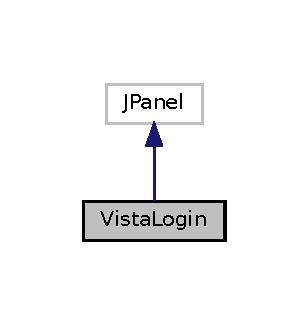
\includegraphics[width=148pt]{class_presentacion_1_1_vista_login__inherit__graph}
\end{center}
\end{figure}


Collaboration diagram for Vista\+Login\+:
\nopagebreak
\begin{figure}[H]
\begin{center}
\leavevmode
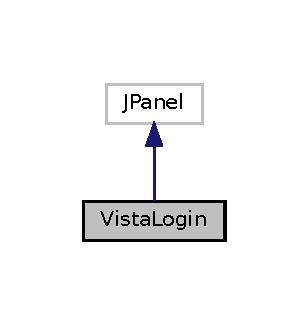
\includegraphics[width=148pt]{class_presentacion_1_1_vista_login__coll__graph}
\end{center}
\end{figure}
\subsection*{Public Member Functions}
\begin{DoxyCompactItemize}
\item 
\mbox{\label{class_presentacion_1_1_vista_login_afb1329298dcf09b9a6becef71d66409b}} 
{\bfseries Vista\+Login} (\textbf{ Vista\+Gestion\+Perfil} gp)
\end{DoxyCompactItemize}


\subsection{Detailed Description}
Clase que extiende J\+Panel que inicializa, gestiona y modifica el panel de la \doxyref{Vista\+Gestion\+Perfil}{p.}{class_presentacion_1_1_vista_gestion_perfil} para iniciar sesión. 

Definition at line 22 of file Vista\+Login.\+java.



The documentation for this class was generated from the following file\+:\begin{DoxyCompactItemize}
\item 
src/\+Presentacion/\textbf{ Vista\+Login.\+java}\end{DoxyCompactItemize}

\section{Vista\+Menu\+Principal Class Reference}
\label{class_presentacion_1_1_vista_menu_principal}\index{Vista\+Menu\+Principal@{Vista\+Menu\+Principal}}


Clase que extiende J\+Panel que inicializa, gestiona y modifica el panel de la \doxyref{Vista\+Principal}{p.}{class_presentacion_1_1_vista_principal} para mostrar el menú principal.  




Inheritance diagram for Vista\+Menu\+Principal\+:
\nopagebreak
\begin{figure}[H]
\begin{center}
\leavevmode
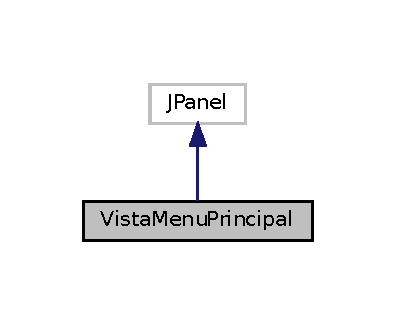
\includegraphics[width=190pt]{class_presentacion_1_1_vista_menu_principal__inherit__graph}
\end{center}
\end{figure}


Collaboration diagram for Vista\+Menu\+Principal\+:
\nopagebreak
\begin{figure}[H]
\begin{center}
\leavevmode
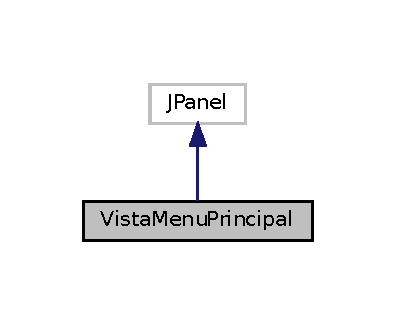
\includegraphics[width=190pt]{class_presentacion_1_1_vista_menu_principal__coll__graph}
\end{center}
\end{figure}
\subsection*{Public Member Functions}
\begin{DoxyCompactItemize}
\item 
\mbox{\label{class_presentacion_1_1_vista_menu_principal_a193026f0fe44beaa3a4b311179200d24}} 
void {\bfseries set\+Usuario} (String User)
\end{DoxyCompactItemize}


\subsection{Detailed Description}
Clase que extiende J\+Panel que inicializa, gestiona y modifica el panel de la \doxyref{Vista\+Principal}{p.}{class_presentacion_1_1_vista_principal} para mostrar el menú principal. 

Definition at line 21 of file Vista\+Menu\+Principal.\+java.



The documentation for this class was generated from the following file\+:\begin{DoxyCompactItemize}
\item 
src/\+Presentacion/\textbf{ Vista\+Menu\+Principal.\+java}\end{DoxyCompactItemize}

\section{Vista\+Nueva\+Partida Class Reference}
\label{class_presentacion_1_1_vista_nueva_partida}\index{Vista\+Nueva\+Partida@{Vista\+Nueva\+Partida}}


Clase que extiende J\+Panel que inicializa, gestiona y modifica el panel de la \doxyref{Vista\+Principal}{p.}{class_presentacion_1_1_vista_principal} para jugar una nueva partida.  




Inheritance diagram for Vista\+Nueva\+Partida\+:
\nopagebreak
\begin{figure}[H]
\begin{center}
\leavevmode
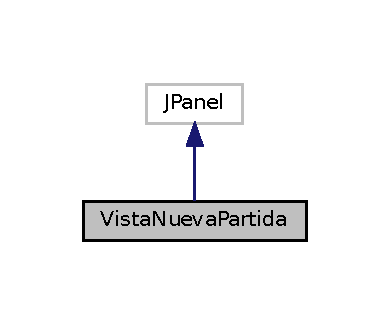
\includegraphics[width=187pt]{class_presentacion_1_1_vista_nueva_partida__inherit__graph}
\end{center}
\end{figure}


Collaboration diagram for Vista\+Nueva\+Partida\+:
\nopagebreak
\begin{figure}[H]
\begin{center}
\leavevmode
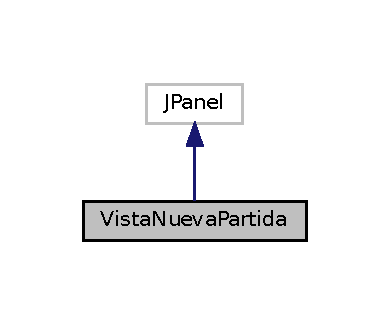
\includegraphics[width=187pt]{class_presentacion_1_1_vista_nueva_partida__coll__graph}
\end{center}
\end{figure}
\subsection*{Public Member Functions}
\begin{DoxyCompactItemize}
\item 
\textbf{ Vista\+Nueva\+Partida} ()
\item 
\mbox{\label{class_presentacion_1_1_vista_nueva_partida_a6a904a8f3955be9a9f561cbb4d1125bf}} 
{\bfseries Vista\+Nueva\+Partida} (\textbf{ Vista\+Principal} vista\+Principal)
\end{DoxyCompactItemize}


\subsection{Detailed Description}
Clase que extiende J\+Panel que inicializa, gestiona y modifica el panel de la \doxyref{Vista\+Principal}{p.}{class_presentacion_1_1_vista_principal} para jugar una nueva partida. 

Definition at line 21 of file Vista\+Nueva\+Partida.\+java.



\subsection{Constructor \& Destructor Documentation}
\mbox{\label{class_presentacion_1_1_vista_nueva_partida_aaea054fc37e0853f8698578118d7aa27}} 
\index{Presentacion\+::\+Vista\+Nueva\+Partida@{Presentacion\+::\+Vista\+Nueva\+Partida}!Vista\+Nueva\+Partida@{Vista\+Nueva\+Partida}}
\index{Vista\+Nueva\+Partida@{Vista\+Nueva\+Partida}!Presentacion\+::\+Vista\+Nueva\+Partida@{Presentacion\+::\+Vista\+Nueva\+Partida}}
\subsubsection{Vista\+Nueva\+Partida()}
{\footnotesize\ttfamily \textbf{ Vista\+Nueva\+Partida} (\begin{DoxyParamCaption}{ }\end{DoxyParamCaption})\hspace{0.3cm}{\ttfamily [inline]}}

Creates new form \doxyref{Vista\+Crear\+Kakuro}{p.}{class_presentacion_1_1_vista_crear_kakuro} 

Definition at line 26 of file Vista\+Nueva\+Partida.\+java.



The documentation for this class was generated from the following file\+:\begin{DoxyCompactItemize}
\item 
src/\+Presentacion/\textbf{ Vista\+Nueva\+Partida.\+java}\end{DoxyCompactItemize}

\section{Vista\+Partida Class Reference}
\label{class_presentacion_1_1_vista_partida}\index{Vista\+Partida@{Vista\+Partida}}


Clase que extiende J\+Panel que inicializa, gestiona y modifica el panel de la \doxyref{Vista\+Principal}{p.}{class_presentacion_1_1_vista_principal} para jugar una partida.  




Inheritance diagram for Vista\+Partida\+:
\nopagebreak
\begin{figure}[H]
\begin{center}
\leavevmode
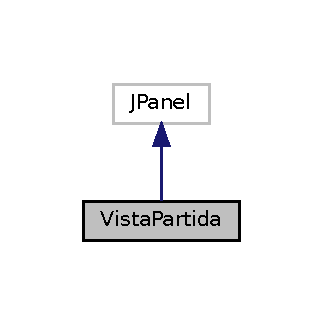
\includegraphics[width=155pt]{class_presentacion_1_1_vista_partida__inherit__graph}
\end{center}
\end{figure}


Collaboration diagram for Vista\+Partida\+:
\nopagebreak
\begin{figure}[H]
\begin{center}
\leavevmode
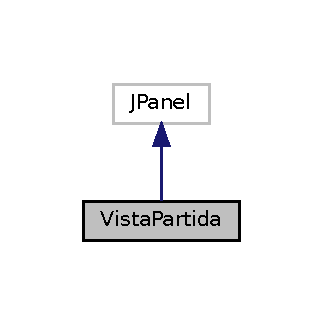
\includegraphics[width=155pt]{class_presentacion_1_1_vista_partida__coll__graph}
\end{center}
\end{figure}
\subsection*{Public Member Functions}
\begin{DoxyCompactItemize}
\item 
\textbf{ Vista\+Partida} ()
\item 
\mbox{\label{class_presentacion_1_1_vista_partida_a147ac103cada9d466b0008516069facf}} 
{\bfseries Vista\+Partida} (\textbf{ Vista\+Principal} vista\+Principal)
\end{DoxyCompactItemize}


\subsection{Detailed Description}
Clase que extiende J\+Panel que inicializa, gestiona y modifica el panel de la \doxyref{Vista\+Principal}{p.}{class_presentacion_1_1_vista_principal} para jugar una partida. 

Definition at line 21 of file Vista\+Partida.\+java.



\subsection{Constructor \& Destructor Documentation}
\mbox{\label{class_presentacion_1_1_vista_partida_a50dd6e6120626c0405ece0d43ed468ed}} 
\index{Presentacion\+::\+Vista\+Partida@{Presentacion\+::\+Vista\+Partida}!Vista\+Partida@{Vista\+Partida}}
\index{Vista\+Partida@{Vista\+Partida}!Presentacion\+::\+Vista\+Partida@{Presentacion\+::\+Vista\+Partida}}
\subsubsection{Vista\+Partida()}
{\footnotesize\ttfamily \textbf{ Vista\+Partida} (\begin{DoxyParamCaption}{ }\end{DoxyParamCaption})\hspace{0.3cm}{\ttfamily [inline]}}

Creates new form \doxyref{Vista\+Partida}{p.}{class_presentacion_1_1_vista_partida} 

Definition at line 26 of file Vista\+Partida.\+java.



The documentation for this class was generated from the following file\+:\begin{DoxyCompactItemize}
\item 
src/\+Presentacion/Vista\+Partida.\+java\end{DoxyCompactItemize}

\section{Vista\+Principal Class Reference}
\label{class_presentacion_1_1_vista_principal}\index{Vista\+Principal@{Vista\+Principal}}


Clase que inicializa todos los paneles de la vista, además de gestionar el cambio entre paneles y su correcto funcionamiento. también transmite y recibe las solicitudes de datos y sus resultados para los paneles que gestiona.  




Collaboration diagram for Vista\+Principal\+:
\nopagebreak
\begin{figure}[H]
\begin{center}
\leavevmode
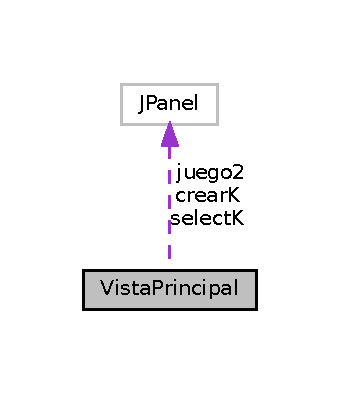
\includegraphics[width=163pt]{class_presentacion_1_1_vista_principal__coll__graph}
\end{center}
\end{figure}
\subsection*{Public Member Functions}
\begin{DoxyCompactItemize}
\item 
\mbox{\label{class_presentacion_1_1_vista_principal_a8d40e08d072012a7d130ceba47e34f50}} 
void {\bfseries change\+To\+Menu} ()
\item 
\mbox{\label{class_presentacion_1_1_vista_principal_ab394ef525ce8cb59259741fbdd89e787}} 
void {\bfseries change\+To\+Partida} ()
\item 
\mbox{\label{class_presentacion_1_1_vista_principal_a860073866cf68025051d2ddea38ec65e}} 
void {\bfseries change\+To\+Juego} ()
\item 
\mbox{\label{class_presentacion_1_1_vista_principal_ad099c0dbb4e84ea7dc48ac333d20ba52}} 
void {\bfseries change\+To\+Cargar} ()
\item 
\mbox{\label{class_presentacion_1_1_vista_principal_a2b9b84bfac2083a7263563e881a38320}} 
void {\bfseries change\+To\+Perfiles} ()
\item 
\mbox{\label{class_presentacion_1_1_vista_principal_a2dbbdd75f198b2e31506e45847f67ff2}} 
void {\bfseries change\+To\+Nueva\+Partida} ()
\item 
\mbox{\label{class_presentacion_1_1_vista_principal_ae368d68edbcc9518c455b7e73e20d81f}} 
void {\bfseries change\+To\+Seleccionar\+Kakuro} ()
\item 
\mbox{\label{class_presentacion_1_1_vista_principal_ab7a5923c6306eb7938e8db1c1bd85644}} 
void {\bfseries change\+To\+Crear\+Kakuro} ()
\item 
\mbox{\label{class_presentacion_1_1_vista_principal_a9e4e0c42aef188b4d526a0ca01e373a5}} 
void {\bfseries change\+To\+Ranking} ()
\item 
\mbox{\label{class_presentacion_1_1_vista_principal_ad039a1881f9a01b0d6ba547505b4ceb4}} 
void {\bfseries desactivar} ()
\item 
\mbox{\label{class_presentacion_1_1_vista_principal_add12112d8694e477589f03ebebc3ff67}} 
void {\bfseries activar} ()
\item 
\mbox{\label{class_presentacion_1_1_vista_principal_ae147a1faf581c3727242c494a29c27b3}} 
\textbf{ Ctrl\+Presentacion} {\bfseries get\+Ctrl\+Presentacion} ()
\item 
\mbox{\label{class_presentacion_1_1_vista_principal_aa2ce56241163b9f202ac684743d12e9b}} 
String {\bfseries get\+Usuario} ()
\item 
\mbox{\label{class_presentacion_1_1_vista_principal_a40d595637eecfc198239a1cd1c05fbce}} 
void {\bfseries set\+Usuario} (String Usuario)
\item 
\mbox{\label{class_presentacion_1_1_vista_principal_a97c11c0e43c900c7cc2dfc4d4ed2ccb6}} 
String [$\,$] {\bfseries Cargar\+I\+Ds} ()
\item 
\mbox{\label{class_presentacion_1_1_vista_principal_a45ebd0e10cf0731cbd580006a2b9e365}} 
String [$\,$] {\bfseries get\+\_\+lista\+\_\+kakuro} ()
\item 
\mbox{\label{class_presentacion_1_1_vista_principal_a9c44d939388c8198de20e1255cd41313}} 
String {\bfseries get\+Ranking} ()
\item 
\mbox{\label{class_presentacion_1_1_vista_principal_ab5947b202b60acac8287ea0a3986af40}} 
void {\bfseries set\+Kakuroenjuego} (int id)
\item 
\mbox{\label{class_presentacion_1_1_vista_principal_af1096a92a8f67defc858f0559ec4adaa}} 
void {\bfseries set\+Tablero\+With\+Dimensions} (int dim)
\end{DoxyCompactItemize}


\subsection{Detailed Description}
Clase que inicializa todos los paneles de la vista, además de gestionar el cambio entre paneles y su correcto funcionamiento. también transmite y recibe las solicitudes de datos y sus resultados para los paneles que gestiona. 

Definition at line 33 of file Vista\+Principal.\+java.



The documentation for this class was generated from the following file\+:\begin{DoxyCompactItemize}
\item 
src/\+Presentacion/\textbf{ Vista\+Principal.\+java}\end{DoxyCompactItemize}

\section{Vista\+Ranking Class Reference}
\label{class_presentacion_1_1_vista_ranking}\index{Vista\+Ranking@{Vista\+Ranking}}


Clase que extiende J\+Panel que inicializa, gestiona y modifica el panel de la \doxyref{Vista\+Principal}{p.}{class_presentacion_1_1_vista_principal} para consultar el ranking.  




Inheritance diagram for Vista\+Ranking\+:
\nopagebreak
\begin{figure}[H]
\begin{center}
\leavevmode
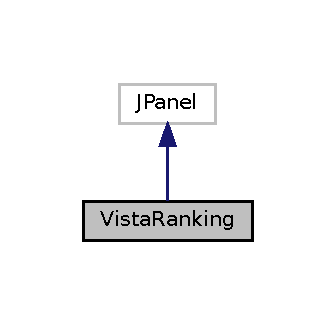
\includegraphics[width=161pt]{class_presentacion_1_1_vista_ranking__inherit__graph}
\end{center}
\end{figure}


Collaboration diagram for Vista\+Ranking\+:
\nopagebreak
\begin{figure}[H]
\begin{center}
\leavevmode
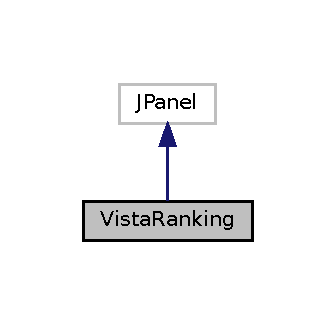
\includegraphics[width=161pt]{class_presentacion_1_1_vista_ranking__coll__graph}
\end{center}
\end{figure}
\subsection*{Public Member Functions}
\begin{DoxyCompactItemize}
\item 
\textbf{ Vista\+Ranking} ()
\item 
\mbox{\label{class_presentacion_1_1_vista_ranking_aa8c670b17237fbfb7cdc91eed6e2ebbf}} 
{\bfseries Vista\+Ranking} (\textbf{ Vista\+Principal} vista\+Principal)
\end{DoxyCompactItemize}


\subsection{Detailed Description}
Clase que extiende J\+Panel que inicializa, gestiona y modifica el panel de la \doxyref{Vista\+Principal}{p.}{class_presentacion_1_1_vista_principal} para consultar el ranking. 

Definition at line 22 of file Vista\+Ranking.\+java.



\subsection{Constructor \& Destructor Documentation}
\mbox{\label{class_presentacion_1_1_vista_ranking_a9b64b7a79aeaa3bd68333914719fd8f8}} 
\index{Presentacion\+::\+Vista\+Ranking@{Presentacion\+::\+Vista\+Ranking}!Vista\+Ranking@{Vista\+Ranking}}
\index{Vista\+Ranking@{Vista\+Ranking}!Presentacion\+::\+Vista\+Ranking@{Presentacion\+::\+Vista\+Ranking}}
\subsubsection{Vista\+Ranking()}
{\footnotesize\ttfamily \textbf{ Vista\+Ranking} (\begin{DoxyParamCaption}{ }\end{DoxyParamCaption})\hspace{0.3cm}{\ttfamily [inline]}}

Creates new form \doxyref{Vista\+Ranking}{p.}{class_presentacion_1_1_vista_ranking} 

Definition at line 28 of file Vista\+Ranking.\+java.



The documentation for this class was generated from the following file\+:\begin{DoxyCompactItemize}
\item 
src/\+Presentacion/\textbf{ Vista\+Ranking.\+java}\end{DoxyCompactItemize}

\section{Vista\+Seleccionar\+Kakuro Class Reference}
\label{class_presentacion_1_1_vista_seleccionar_kakuro}\index{Vista\+Seleccionar\+Kakuro@{Vista\+Seleccionar\+Kakuro}}


Clase que extiende J\+Panel que inicializa, gestiona y modifica el panel de la \doxyref{Vista\+Principal}{p.}{class_presentacion_1_1_vista_principal} para Seleccionar un kakuro ya existente mediante su ID.  




Inheritance diagram for Vista\+Seleccionar\+Kakuro\+:
\nopagebreak
\begin{figure}[H]
\begin{center}
\leavevmode
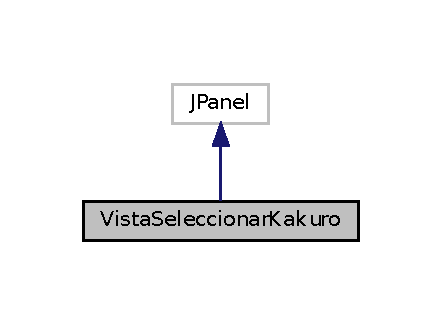
\includegraphics[width=212pt]{class_presentacion_1_1_vista_seleccionar_kakuro__inherit__graph}
\end{center}
\end{figure}


Collaboration diagram for Vista\+Seleccionar\+Kakuro\+:
\nopagebreak
\begin{figure}[H]
\begin{center}
\leavevmode
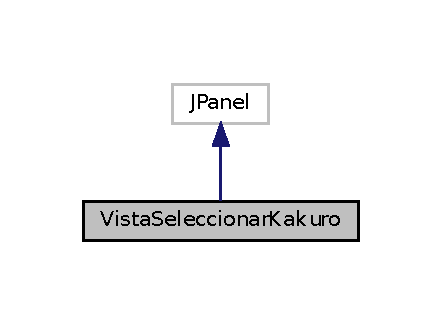
\includegraphics[width=212pt]{class_presentacion_1_1_vista_seleccionar_kakuro__coll__graph}
\end{center}
\end{figure}
\subsection*{Public Member Functions}
\begin{DoxyCompactItemize}
\item 
\textbf{ Vista\+Seleccionar\+Kakuro} ()
\item 
\mbox{\label{class_presentacion_1_1_vista_seleccionar_kakuro_a4366ca2460b418db699c64f1555ecc1f}} 
{\bfseries Vista\+Seleccionar\+Kakuro} (\textbf{ Vista\+Principal} vista\+Principal)
\item 
\mbox{\label{class_presentacion_1_1_vista_seleccionar_kakuro_a6b4e768cdd47ad0b5e9bcb6d2920e78c}} 
void {\bfseries actualizar\+Lista} ()
\end{DoxyCompactItemize}


\subsection{Detailed Description}
Clase que extiende J\+Panel que inicializa, gestiona y modifica el panel de la \doxyref{Vista\+Principal}{p.}{class_presentacion_1_1_vista_principal} para Seleccionar un kakuro ya existente mediante su ID. 

Definition at line 22 of file Vista\+Seleccionar\+Kakuro.\+java.



\subsection{Constructor \& Destructor Documentation}
\mbox{\label{class_presentacion_1_1_vista_seleccionar_kakuro_a9a9f2c26cc6e9023b31b4f10cc4a9856}} 
\index{Presentacion\+::\+Vista\+Seleccionar\+Kakuro@{Presentacion\+::\+Vista\+Seleccionar\+Kakuro}!Vista\+Seleccionar\+Kakuro@{Vista\+Seleccionar\+Kakuro}}
\index{Vista\+Seleccionar\+Kakuro@{Vista\+Seleccionar\+Kakuro}!Presentacion\+::\+Vista\+Seleccionar\+Kakuro@{Presentacion\+::\+Vista\+Seleccionar\+Kakuro}}
\subsubsection{Vista\+Seleccionar\+Kakuro()}
{\footnotesize\ttfamily \textbf{ Vista\+Seleccionar\+Kakuro} (\begin{DoxyParamCaption}{ }\end{DoxyParamCaption})\hspace{0.3cm}{\ttfamily [inline]}}

Creates new form \doxyref{Vista\+Seleccionar\+Kakuro}{p.}{class_presentacion_1_1_vista_seleccionar_kakuro} 

Definition at line 28 of file Vista\+Seleccionar\+Kakuro.\+java.



The documentation for this class was generated from the following file\+:\begin{DoxyCompactItemize}
\item 
src/\+Presentacion/\textbf{ Vista\+Seleccionar\+Kakuro.\+java}\end{DoxyCompactItemize}

\section{Vista\+Sign\+Up Class Reference}
\label{class_presentacion_1_1_vista_sign_up}\index{Vista\+Sign\+Up@{Vista\+Sign\+Up}}


Inheritance diagram for Vista\+Sign\+Up\+:
\nopagebreak
\begin{figure}[H]
\begin{center}
\leavevmode
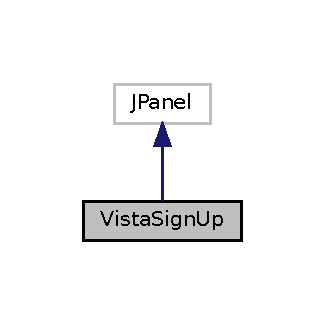
\includegraphics[width=156pt]{class_presentacion_1_1_vista_sign_up__inherit__graph}
\end{center}
\end{figure}


Collaboration diagram for Vista\+Sign\+Up\+:
\nopagebreak
\begin{figure}[H]
\begin{center}
\leavevmode
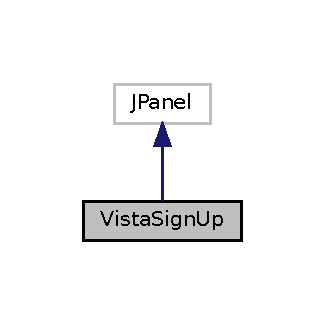
\includegraphics[width=156pt]{class_presentacion_1_1_vista_sign_up__coll__graph}
\end{center}
\end{figure}
\subsection*{Public Member Functions}
\begin{DoxyCompactItemize}
\item 
\mbox{\label{class_presentacion_1_1_vista_sign_up_ae1ca508ec6563c18e901dbb807071fc5}} 
{\bfseries Vista\+Sign\+Up} (\textbf{ Vista\+Gestion\+Perfil} gp)
\end{DoxyCompactItemize}


\subsection{Detailed Description}


Definition at line 21 of file Vista\+Sign\+Up.\+java.



The documentation for this class was generated from the following file\+:\begin{DoxyCompactItemize}
\item 
src/\+Presentacion/\textbf{ Vista\+Sign\+Up.\+java}\end{DoxyCompactItemize}

\chapter{File Documentation}
\section{src/\+Dominio/clases/\+Casilla.java File Reference}
\label{_casilla_8java}\index{src/\+Dominio/clases/\+Casilla.\+java@{src/\+Dominio/clases/\+Casilla.\+java}}


Archivo que implementa la clase Casilla.  


\subsection*{Data Structures}
\begin{DoxyCompactItemize}
\item 
class \textbf{ Casilla}
\begin{DoxyCompactList}\small\item\em Clase que representa una \doxyref{Casilla}{p.}{class_dominio_1_1clases_1_1_casilla} de un tablero de un \doxyref{Kakuro}{p.}{class_dominio_1_1clases_1_1_kakuro}. \end{DoxyCompactList}\item 
enum {\bfseries Casilla.\+Tipo}
\end{DoxyCompactItemize}


\subsection{Detailed Description}
Archivo que implementa la clase Casilla. 

\begin{DoxyDate}{Date}
20-\/12-\/2020 
\end{DoxyDate}
\begin{DoxyAuthor}{Author}
Jesus Benitez 
\end{DoxyAuthor}

\section{src/\+Dominio/clases/\+Kakuro.java File Reference}
\label{_kakuro_8java}\index{src/\+Dominio/clases/\+Kakuro.\+java@{src/\+Dominio/clases/\+Kakuro.\+java}}


Archivo que implementa la clase Kakuro.  


\subsection*{Data Structures}
\begin{DoxyCompactItemize}
\item 
class \textbf{ Kakuro}
\begin{DoxyCompactList}\small\item\em Clase que representa un kakuro. Contiene su tablero tanto información sobre el mismo. \end{DoxyCompactList}\end{DoxyCompactItemize}


\subsection{Detailed Description}
Archivo que implementa la clase Kakuro. 

\begin{DoxyDate}{Date}
20-\/12-\/2020 
\end{DoxyDate}
\begin{DoxyAuthor}{Author}
Mauro Garcia 
\end{DoxyAuthor}

\section{src/\+Dominio/clases/\+Kakuro\+\_\+\+Game.java File Reference}
\label{_kakuro___game_8java}\index{src/\+Dominio/clases/\+Kakuro\+\_\+\+Game.\+java@{src/\+Dominio/clases/\+Kakuro\+\_\+\+Game.\+java}}


Archivo principal del programa.  


\subsection*{Data Structures}
\begin{DoxyCompactItemize}
\item 
class \textbf{ Kakuro\+\_\+\+Game}
\end{DoxyCompactItemize}


\subsection{Detailed Description}
Archivo principal del programa. 

\begin{DoxyDate}{Date}
20-\/12-\/2020 
\end{DoxyDate}
\begin{DoxyAuthor}{Author}
David Nogales 
\end{DoxyAuthor}

\section{src/\+Dominio/clases/partida.java File Reference}
\label{partida_8java}\index{src/\+Dominio/clases/partida.\+java@{src/\+Dominio/clases/partida.\+java}}


Archivo que implementa la clase partida.  


\subsection*{Data Structures}
\begin{DoxyCompactItemize}
\item 
class \textbf{ partida}
\begin{DoxyCompactList}\small\item\em Clase que representa una partida. Cada partida consiste en el id del usuario que la guarda, un identificador de partida, el tiempo transcurrido y el \doxyref{Kakuro}{p.}{class_dominio_1_1clases_1_1_kakuro} en juego. \end{DoxyCompactList}\end{DoxyCompactItemize}


\subsection{Detailed Description}
Archivo que implementa la clase partida. 

\begin{DoxyDate}{Date}
20-\/12-\/2020 
\end{DoxyDate}
\begin{DoxyAuthor}{Author}
Pere Masip 
\end{DoxyAuthor}

\section{src/\+Dominio/controladores/\+Capa\+Dominio\+Kakuro.java File Reference}
\label{_capa_dominio_kakuro_8java}\index{src/\+Dominio/controladores/\+Capa\+Dominio\+Kakuro.\+java@{src/\+Dominio/controladores/\+Capa\+Dominio\+Kakuro.\+java}}


archivo que contiene las funcionalidades principales del programa  


\subsection*{Data Structures}
\begin{DoxyCompactItemize}
\item 
class \textbf{ Capa\+Dominio\+Kakuro}
\begin{DoxyCompactList}\small\item\em clase donde implementamos las funcionalidades principales del programa, siendo estas validar, generar y solucionar un Kakuro. \end{DoxyCompactList}\end{DoxyCompactItemize}


\subsection{Detailed Description}
archivo que contiene las funcionalidades principales del programa 

\begin{DoxyDate}{Date}
20-\/12-\/2020 
\end{DoxyDate}
\begin{DoxyAuthor}{Author}
Pere Masip 
\end{DoxyAuthor}

\section{src/\+Dominio/controladores/\+Ctrl\+Capa\+Dominio.java File Reference}
\label{_ctrl_capa_dominio_8java}\index{src/\+Dominio/controladores/\+Ctrl\+Capa\+Dominio.\+java@{src/\+Dominio/controladores/\+Ctrl\+Capa\+Dominio.\+java}}


Controlador que interactúa con la capa de dominio y se encarga de pasar datos con las demás capas.  


\subsection*{Data Structures}
\begin{DoxyCompactItemize}
\item 
class \textbf{ Ctrl\+Capa\+Dominio}
\begin{DoxyCompactList}\small\item\em Clase que se utiliza como intermediaria entre presentacion y persistencia. Transforma los datos que recibe de persistencia y se los pasa a presentacion. \end{DoxyCompactList}\end{DoxyCompactItemize}


\subsection{Detailed Description}
Controlador que interactúa con la capa de dominio y se encarga de pasar datos con las demás capas. 

\begin{DoxyDate}{Date}
20-\/12-\/2020 
\end{DoxyDate}
\begin{DoxyAuthor}{Author}
Pere Masip 
\end{DoxyAuthor}

\section{src/\+Persistencia/\+Ctrl\+Kakuro.java File Reference}
\label{_ctrl_kakuro_8java}\index{src/\+Persistencia/\+Ctrl\+Kakuro.\+java@{src/\+Persistencia/\+Ctrl\+Kakuro.\+java}}


Archivo que implementa la lectura y escritura de Kakuros en disco.  


\subsection*{Data Structures}
\begin{DoxyCompactItemize}
\item 
class \textbf{ Ctrl\+Kakuro}
\begin{DoxyCompactList}\small\item\em Clase que implementa la lectura y escritura de Kakuros en disco. \end{DoxyCompactList}\end{DoxyCompactItemize}


\subsection{Detailed Description}
Archivo que implementa la lectura y escritura de Kakuros en disco. 

\begin{DoxyDate}{Date}
20-\/12-\/2020 
\end{DoxyDate}
\begin{DoxyAuthor}{Author}
Mauro Garcia 
\end{DoxyAuthor}

\section{src/\+Persistencia/\+Ctrl\+Partida.java File Reference}
\label{_ctrl_partida_8java}\index{src/\+Persistencia/\+Ctrl\+Partida.\+java@{src/\+Persistencia/\+Ctrl\+Partida.\+java}}


Archivo que implementa la lectura y escritura de partidas en disco.  


\subsection*{Data Structures}
\begin{DoxyCompactItemize}
\item 
class \textbf{ Ctrl\+Partida}
\begin{DoxyCompactList}\small\item\em Clase que implementa la lectura y escritura de partidas en disco. \end{DoxyCompactList}\end{DoxyCompactItemize}


\subsection{Detailed Description}
Archivo que implementa la lectura y escritura de partidas en disco. 

\begin{DoxyDate}{Date}
20-\/12-\/2020 
\end{DoxyDate}
\begin{DoxyAuthor}{Author}
Mauro Garcia 
\end{DoxyAuthor}

\section{src/\+Persistencia/\+Ctrl\+Persistencia.java File Reference}
\label{_ctrl_persistencia_8java}\index{src/\+Persistencia/\+Ctrl\+Persistencia.\+java@{src/\+Persistencia/\+Ctrl\+Persistencia.\+java}}


Archivo que implementa el controlador de la capa de persistencia.  


\subsection*{Data Structures}
\begin{DoxyCompactItemize}
\item 
class \textbf{ Ctrl\+Persistencia}
\begin{DoxyCompactList}\small\item\em Clase que se encarga de recibir consultas y enviar datos a las demás capas de proyecto. éstas consultas las llevará a la clase indicada y devolverá su resultado. \end{DoxyCompactList}\end{DoxyCompactItemize}


\subsection{Detailed Description}
Archivo que implementa el controlador de la capa de persistencia. 

\begin{DoxyDate}{Date}
20-\/12-\/2020 
\end{DoxyDate}
\begin{DoxyAuthor}{Author}
Jesus Benitez 
\end{DoxyAuthor}

\section{src/\+Persistencia/\+Ctrl\+Ranking.java File Reference}
\label{_ctrl_ranking_8java}\index{src/\+Persistencia/\+Ctrl\+Ranking.\+java@{src/\+Persistencia/\+Ctrl\+Ranking.\+java}}


Archivo que implementa la lectura y escritura del Ranking en disco.  


\subsection*{Data Structures}
\begin{DoxyCompactItemize}
\item 
class \textbf{ Ctrl\+Ranking}
\begin{DoxyCompactList}\small\item\em Clase que implementa la lectura y escritura del Ranking en disco. \end{DoxyCompactList}\end{DoxyCompactItemize}


\subsection{Detailed Description}
Archivo que implementa la lectura y escritura del Ranking en disco. 

\begin{DoxyDate}{Date}
20-\/12-\/2020 
\end{DoxyDate}
\begin{DoxyAuthor}{Author}
Jesus Benitez 
\end{DoxyAuthor}

\section{src/\+Persistencia/\+Ctrl\+Registro.java File Reference}
\label{_ctrl_registro_8java}\index{src/\+Persistencia/\+Ctrl\+Registro.\+java@{src/\+Persistencia/\+Ctrl\+Registro.\+java}}


Archivo que implementa la lectura y escritura del registro de usuarios en disco.  


\subsection*{Data Structures}
\begin{DoxyCompactItemize}
\item 
class \textbf{ Ctrl\+Registro}
\begin{DoxyCompactList}\small\item\em Clase que implementa la lectura y escritura del registro de usuarios en disco. \end{DoxyCompactList}\end{DoxyCompactItemize}


\subsection{Detailed Description}
Archivo que implementa la lectura y escritura del registro de usuarios en disco. 

\begin{DoxyDate}{Date}
20-\/12-\/2020 
\end{DoxyDate}
\begin{DoxyAuthor}{Author}
Mauro Garcia 
\end{DoxyAuthor}

\section{src/\+Presentacion/\+Ctrl\+Presentacion.java File Reference}
\label{_ctrl_presentacion_8java}\index{src/\+Presentacion/\+Ctrl\+Presentacion.\+java@{src/\+Presentacion/\+Ctrl\+Presentacion.\+java}}


Controlador de la capa de presentación.  


\subsection*{Data Structures}
\begin{DoxyCompactItemize}
\item 
class \textbf{ Ctrl\+Presentacion}
\begin{DoxyCompactList}\small\item\em Clase que inicializa todos los controladores de presentación y contiene las funcionalidades necesarias para llevar a cabo la función explicada anteriormente. \end{DoxyCompactList}\end{DoxyCompactItemize}


\subsection{Detailed Description}
Controlador de la capa de presentación. 

Dialogo para guardar partida.

\begin{DoxyDate}{Date}
20-\/12-\/2020 
\end{DoxyDate}
\begin{DoxyAuthor}{Author}
David Nogales Controlador que se encarga de gestionar las peticiones de datos de las capas de presentación, mandarlas a la capa de dominio, recoger los resultados y llevarlos de vuelta a la vista que hace la solicitud.
\end{DoxyAuthor}
\begin{DoxyDate}{Date}
20-\/12-\/2020 
\end{DoxyDate}
\begin{DoxyAuthor}{Author}
David Nogales Dialogo para poner nombre a una partida guardada 
\end{DoxyAuthor}

\section{src/\+Presentacion/\+Kakuro\+Grid.java File Reference}
\label{_kakuro_grid_8java}\index{src/\+Presentacion/\+Kakuro\+Grid.\+java@{src/\+Presentacion/\+Kakuro\+Grid.\+java}}


panel que contiene el Kakuro en Juego  


\subsection*{Data Structures}
\begin{DoxyCompactItemize}
\item 
class {\bfseries Kakuro\+Grid}
\begin{DoxyCompactList}\small\item\em Clase que extiende J\+Panel que inicializa, gestiona y modifica el kakuro en Juego y sus casillas. \end{DoxyCompactList}\end{DoxyCompactItemize}


\subsection{Detailed Description}
panel que contiene el Kakuro en Juego 

\begin{DoxyDate}{Date}
20-\/12-\/2020 
\end{DoxyDate}
\begin{DoxyAuthor}{Author}
David Nogales Panel que contiene el Kakuro en Juego, además de gestionar cada una de las casillas que contiene. 
\end{DoxyAuthor}

\section{src/\+Presentacion/\+Kakuro\+Panel.java File Reference}
\label{_kakuro_panel_8java}\index{src/\+Presentacion/\+Kakuro\+Panel.\+java@{src/\+Presentacion/\+Kakuro\+Panel.\+java}}


panel correspondiente a una casilla del Kakuro en Juego.  


\subsection*{Data Structures}
\begin{DoxyCompactItemize}
\item 
class {\bfseries Kakuro\+Panel}
\end{DoxyCompactItemize}


\subsection{Detailed Description}
panel correspondiente a una casilla del Kakuro en Juego. 

\begin{DoxyDate}{Date}
20-\/12-\/2020 
\end{DoxyDate}
\begin{DoxyAuthor}{Author}
David Nogales Panel que contiene una casilla del Kakuro en juego, desde la que se piden comprobaciones de movimientos a Dominio y cambia su comportamiento dependiendo del resultado. 
\end{DoxyAuthor}

\section{src/\+Presentacion/\+Vista\+Cargar\+Partida.java File Reference}
\label{_vista_cargar_partida_8java}\index{src/\+Presentacion/\+Vista\+Cargar\+Partida.\+java@{src/\+Presentacion/\+Vista\+Cargar\+Partida.\+java}}


Panel que gestiona la sección de Vista\+Principal para cargar Partidas.  


\subsection*{Data Structures}
\begin{DoxyCompactItemize}
\item 
class \textbf{ Vista\+Cargar\+Partida}
\begin{DoxyCompactList}\small\item\em Clase que extiende J\+Panel que inicializa, gestiona y modifica el panel de la \doxyref{Vista\+Principal}{p.}{class_presentacion_1_1_vista_principal} para Cargar Partidas. \end{DoxyCompactList}\end{DoxyCompactItemize}


\subsection{Detailed Description}
Panel que gestiona la sección de Vista\+Principal para cargar Partidas. 

\begin{DoxyDate}{Date}
20-\/12-\/2020 
\end{DoxyDate}
\begin{DoxyAuthor}{Author}
David Nogales dependiendo del resultado de consultar la lista de partidas del usuario que inicia sesión, el usuario deberá seleccionar una de las partidas en caso de que existan y presionar cargar. 
\end{DoxyAuthor}

\section{src/\+Presentacion/\+Vista\+Crear\+Kakuro.java File Reference}
\label{_vista_crear_kakuro_8java}\index{src/\+Presentacion/\+Vista\+Crear\+Kakuro.\+java@{src/\+Presentacion/\+Vista\+Crear\+Kakuro.\+java}}


Panel que gestiona la sección de Vista\+Principal para crear un nuevo Kakuro.  


\subsection*{Data Structures}
\begin{DoxyCompactItemize}
\item 
class \textbf{ Vista\+Crear\+Kakuro}
\begin{DoxyCompactList}\small\item\em Clase que extiende J\+Panel que inicializa, gestiona y modifica el panel de la \doxyref{Vista\+Principal}{p.}{class_presentacion_1_1_vista_principal} para Crear Kakuros. \end{DoxyCompactList}\end{DoxyCompactItemize}


\subsection{Detailed Description}
Panel que gestiona la sección de Vista\+Principal para crear un nuevo Kakuro. 

\begin{DoxyDate}{Date}
20-\/12-\/2020 
\end{DoxyDate}
\begin{DoxyAuthor}{Author}
David Nogales Panel que muestra al usuario las diferentes opciones de creación de kakuros y realizará las operaciones necesarias segun las opciones que el usuario seleccione. 
\end{DoxyAuthor}

\section{src/\+Presentacion/\+Vista\+Gestion\+Perfil.java File Reference}
\label{_vista_gestion_perfil_8java}\index{src/\+Presentacion/\+Vista\+Gestion\+Perfil.\+java@{src/\+Presentacion/\+Vista\+Gestion\+Perfil.\+java}}


Panel que gestiona la Vista de inicio de sesión y registro en el programa.  


\subsection*{Data Structures}
\begin{DoxyCompactItemize}
\item 
class \textbf{ Vista\+Gestion\+Perfil}
\begin{DoxyCompactList}\small\item\em Clase que inicializa, gestiona y modifica la Vista que controla el inicio de sesión y registro en el programa. \end{DoxyCompactList}\end{DoxyCompactItemize}


\subsection{Detailed Description}
Panel que gestiona la Vista de inicio de sesión y registro en el programa. 

\begin{DoxyDate}{Date}
20-\/12-\/2020 
\end{DoxyDate}
\begin{DoxyAuthor}{Author}
David Nogales Vista que solicita al usuario la información de inicio de sesión y registro y que pide a las capas superiores que comprueben la validez de los valores. 
\end{DoxyAuthor}

\section{src/\+Presentacion/\+Vista\+Kakuro.java File Reference}
\label{_vista_kakuro_8java}\index{src/\+Presentacion/\+Vista\+Kakuro.\+java@{src/\+Presentacion/\+Vista\+Kakuro.\+java}}


Panel que gestiona la sección de Vista\+Principal para Jugar un Kakuro.  


\subsection*{Data Structures}
\begin{DoxyCompactItemize}
\item 
class \textbf{ Vista\+Kakuro}
\begin{DoxyCompactList}\small\item\em Clase que extiende J\+Panel que inicializa, gestiona y modifica el panel de la \doxyref{Vista\+Principal}{p.}{class_presentacion_1_1_vista_principal} para jugar un Kakuro. \end{DoxyCompactList}\end{DoxyCompactItemize}


\subsection{Detailed Description}
Panel que gestiona la sección de Vista\+Principal para Jugar un Kakuro. 

\begin{DoxyDate}{Date}
20-\/12-\/2020 
\end{DoxyDate}
\begin{DoxyAuthor}{Author}
David Nogales Este panel contiene el kakuro en juego y los diferentes botones que dan acceso a otras funcionalidades accesibles durante una partida, como solucionar, guardar, pausar o salir. 
\end{DoxyAuthor}

\section{src/\+Presentacion/\+Vista\+Login.java File Reference}
\label{_vista_login_8java}\index{src/\+Presentacion/\+Vista\+Login.\+java@{src/\+Presentacion/\+Vista\+Login.\+java}}


Panel que gestiona la sección de Vista\+Gestion\+Perfil para iniciar sesión.  


\subsection*{Data Structures}
\begin{DoxyCompactItemize}
\item 
class \textbf{ Vista\+Login}
\begin{DoxyCompactList}\small\item\em Clase que extiende J\+Panel que inicializa, gestiona y modifica el panel de la \doxyref{Vista\+Gestion\+Perfil}{p.}{class_presentacion_1_1_vista_gestion_perfil} para iniciar sesión. \end{DoxyCompactList}\end{DoxyCompactItemize}


\subsection{Detailed Description}
Panel que gestiona la sección de Vista\+Gestion\+Perfil para iniciar sesión. 

Panel que gestiona la sección de Vista\+Principal para jugar una partida.

\begin{DoxyDate}{Date}
20-\/12-\/2020 
\end{DoxyDate}
\begin{DoxyAuthor}{Author}
David Nogales Panel que solicita al usuario su información de inicio de sesión y, en caso de obtenerla, pide a las otras capas que la validen. También tiene un botón para acceder al panel de registro
\end{DoxyAuthor}
\begin{DoxyDate}{Date}
20-\/12-\/2020 
\end{DoxyDate}
\begin{DoxyAuthor}{Author}
David Nogales Panel que permite al usuario crear una nueva partida o cargar una partida en curso. 
\end{DoxyAuthor}

\section{src/\+Presentacion/\+Vista\+Menu\+Principal.java File Reference}
\label{_vista_menu_principal_8java}\index{src/\+Presentacion/\+Vista\+Menu\+Principal.\+java@{src/\+Presentacion/\+Vista\+Menu\+Principal.\+java}}


Panel que gestiona la sección de Vista\+Principal para mostrar el menú principal.  


\subsection*{Data Structures}
\begin{DoxyCompactItemize}
\item 
class \textbf{ Vista\+Menu\+Principal}
\begin{DoxyCompactList}\small\item\em Clase que extiende J\+Panel que inicializa, gestiona y modifica el panel de la \doxyref{Vista\+Principal}{p.}{class_presentacion_1_1_vista_principal} para mostrar el menú principal. \end{DoxyCompactList}\end{DoxyCompactItemize}


\subsection{Detailed Description}
Panel que gestiona la sección de Vista\+Principal para mostrar el menú principal. 

\begin{DoxyDate}{Date}
20-\/12-\/2020 
\end{DoxyDate}
\begin{DoxyAuthor}{Author}
David Nogales Panel que da acceso a las funcionalidades principales del programa\+: Jugar, consultar el ránking y cambiar de perfil. 
\end{DoxyAuthor}

\section{src/\+Presentacion/\+Vista\+Nueva\+Partida.java File Reference}
\label{_vista_nueva_partida_8java}\index{src/\+Presentacion/\+Vista\+Nueva\+Partida.\+java@{src/\+Presentacion/\+Vista\+Nueva\+Partida.\+java}}


Panel que gestiona la sección de Vista\+Principal para jugar una nueva partida.  


\subsection*{Data Structures}
\begin{DoxyCompactItemize}
\item 
class \textbf{ Vista\+Nueva\+Partida}
\begin{DoxyCompactList}\small\item\em Clase que extiende J\+Panel que inicializa, gestiona y modifica el panel de la \doxyref{Vista\+Principal}{p.}{class_presentacion_1_1_vista_principal} para jugar una nueva partida. \end{DoxyCompactList}\end{DoxyCompactItemize}


\subsection{Detailed Description}
Panel que gestiona la sección de Vista\+Principal para jugar una nueva partida. 

\begin{DoxyDate}{Date}
20-\/12-\/2020 
\end{DoxyDate}
\begin{DoxyAuthor}{Author}
David Nogales Panel que muestra al usuario las diferentes opciones para crear una nueva partida\+: crear una partida con un kakuro de la biblioteca o crear un nuevo kakuro y jugarlo. 
\end{DoxyAuthor}

\section{src/\+Presentacion/\+Vista\+Principal.java File Reference}
\label{_vista_principal_8java}\index{src/\+Presentacion/\+Vista\+Principal.\+java@{src/\+Presentacion/\+Vista\+Principal.\+java}}


Vista Principal del programa.  


\subsection*{Data Structures}
\begin{DoxyCompactItemize}
\item 
class \textbf{ Vista\+Principal}
\begin{DoxyCompactList}\small\item\em Clase que inicializa todos los paneles de la vista, además de gestionar el cambio entre paneles y su correcto funcionamiento. también transmite y recibe las solicitudes de datos y sus resultados para los paneles que gestiona. \end{DoxyCompactList}\end{DoxyCompactItemize}


\subsection{Detailed Description}
Vista Principal del programa. 

\begin{DoxyDate}{Date}
20-\/12-\/2020 
\end{DoxyDate}
\begin{DoxyAuthor}{Author}
David Nogales Vista que se muestra nada más acabar el inicio de sesión y que se encarga de mostrar todas las funcionalidades principales del programa 
\end{DoxyAuthor}

\section{src/\+Presentacion/\+Vista\+Ranking.java File Reference}
\label{_vista_ranking_8java}\index{src/\+Presentacion/\+Vista\+Ranking.\+java@{src/\+Presentacion/\+Vista\+Ranking.\+java}}


Panel que gestiona la sección de Vista\+Principal que muestra el ranking.  


\subsection*{Data Structures}
\begin{DoxyCompactItemize}
\item 
class \textbf{ Vista\+Ranking}
\begin{DoxyCompactList}\small\item\em Clase que extiende J\+Panel que inicializa, gestiona y modifica el panel de la \doxyref{Vista\+Principal}{p.}{class_presentacion_1_1_vista_principal} para consultar el ranking. \end{DoxyCompactList}\end{DoxyCompactItemize}


\subsection{Detailed Description}
Panel que gestiona la sección de Vista\+Principal que muestra el ranking. 

\begin{DoxyDate}{Date}
20-\/12-\/2020 
\end{DoxyDate}
\begin{DoxyAuthor}{Author}
David Nogales Panel que permite al usuario consultar el ranking con las puntuaciones totales de los usuarios registrados. 
\end{DoxyAuthor}

\section{src/\+Presentacion/\+Vista\+Seleccionar\+Kakuro.java File Reference}
\label{_vista_seleccionar_kakuro_8java}\index{src/\+Presentacion/\+Vista\+Seleccionar\+Kakuro.\+java@{src/\+Presentacion/\+Vista\+Seleccionar\+Kakuro.\+java}}


Panel que gestiona la sección de Vista\+Principal para Seleccionar un kakuro ya existente mediante su ID.  


\subsection*{Data Structures}
\begin{DoxyCompactItemize}
\item 
class \textbf{ Vista\+Seleccionar\+Kakuro}
\begin{DoxyCompactList}\small\item\em Clase que extiende J\+Panel que inicializa, gestiona y modifica el panel de la \doxyref{Vista\+Principal}{p.}{class_presentacion_1_1_vista_principal} para Seleccionar un kakuro ya existente mediante su ID. \end{DoxyCompactList}\end{DoxyCompactItemize}


\subsection{Detailed Description}
Panel que gestiona la sección de Vista\+Principal para Seleccionar un kakuro ya existente mediante su ID. 

\begin{DoxyDate}{Date}
20-\/12-\/2020 
\end{DoxyDate}
\begin{DoxyAuthor}{Author}
David Nogales Panel que permite al usuario Seleccionar un kakuro ya existente para jugarlo. 
\end{DoxyAuthor}

\section{src/\+Presentacion/\+Vista\+Sign\+Up.java File Reference}
\label{_vista_sign_up_8java}\index{src/\+Presentacion/\+Vista\+Sign\+Up.\+java@{src/\+Presentacion/\+Vista\+Sign\+Up.\+java}}


Panel que gestiona la sección de Vista\+Gestion\+Perfil para registrarse.  


\subsection*{Data Structures}
\begin{DoxyCompactItemize}
\item 
class \textbf{ Vista\+Sign\+Up}
\end{DoxyCompactItemize}


\subsection{Detailed Description}
Panel que gestiona la sección de Vista\+Gestion\+Perfil para registrarse. 

\begin{DoxyDate}{Date}
20-\/12-\/2020 
\end{DoxyDate}
\begin{DoxyAuthor}{Author}
David Nogales Panel que solicita al usuario su información de registro y, en caso de obtenerla, pide a las otras capas que la validen. También tiene un botón para acceder al panel de inicio de sesión 
\end{DoxyAuthor}

%--- End generated contents ---

% Index
\backmatter
\newpage
\phantomsection
\clearemptydoublepage
\addcontentsline{toc}{chapter}{Index}
\printindex

\end{document}
